\chapter{神经细胞的分化与存活} \label{chap:chap46}


在前一章中,我们描述了局部感应信号如何塑造神经管并建立神经系统的早期区域细分:脊髓、后脑、中脑和前脑。
在这里,我们将讨论这些区域内的祖细胞如何分化为神经元和神经胶质细胞(神经系统的两种主要细胞类型)的问题。
成熟的大脑包含数十亿个神经细胞和类似数量的以复杂模式排列的神经胶质细胞,但其前体神经板最初仅包含排列在简单柱状上皮中的数百个细胞。
仅从这一观察来看,显然必须仔细调节神经细胞的产生及其向适当部位的递送。


我们首先讨论一些指定神经元和神经胶质细胞命运的分子。
神经发生的基本机制赋予细胞共同的神经元特性,这些特性在很大程度上独立于它们产生的神经系统区域或它们执行的特定功能。
我们还描述了发育中的神经元变得特化的机制,例如通过获得合成特定神经递质的机制。


接下来我们将讨论神经元如何从它们的起源位置传送到它们的最终目的地。
一个共同的主题是神经元经常“出生”(即成为有丝分裂后)远离它们最终到达的地方,例如,在大脑皮层层或周围神经系统的神经节中。
这种距离需要精心设计的迁移机制,这些机制因神经元类型而异。




在神经元的身份和功能特性开始出现后,额外的发育过程决定了神经元是生还是死。
值得注意的是,哺乳动物神经系统中产生的大约一半神经元会因程序性细胞死亡而丢失。
我们研究了调节神经元存活的因素以及广泛的神经元丢失可能带来的好处。
最后,我们描述了神经细胞中注定要被消除的核心生化途径。



\section{神经祖细胞的增殖涉及对称和不对称细胞分裂}

19 世纪后期的组织学家表明,靠近胚胎大脑脑室腔的神经上皮细胞表现出有丝分裂的特征。
我们现在知道,脑室周围的增殖区是中枢神经系统中神经细胞产生的主要场所。
此外,增殖区中的新生细胞在从这些区域迁移之前,通常会成为神经元或神经胶质细胞的命运。


在胚胎发育的早期阶段,神经管心室区的大多数祖细胞迅速增殖。
这些早期神经祖细胞中有许多具有干细胞的特性:
它们可以产生更多的自身副本,这一过程称为自我更新,并且还可以产生分化的神经元和神经胶质细胞。
在后面的章节中,我们将描述最近的发现,即与胚胎干细胞相似的干细胞也存在于成人大脑中,并且可以用于治疗目的(第~\ref{chap:chap50}~章)。


与其他类型的干细胞一样,神经祖细胞经历细胞分裂的固定程序。
一种细胞分裂模式是对称的:神经干细胞分裂产生两个干细胞,并以这种方式扩大增殖祖细胞的数量。
随着神经上皮细胞的扩张,这种模式在最早的时候占主导地位。
第二种模式是不对称的:祖细胞产生一个分化的女儿和另一个保留其干细胞样特性的女儿。
这种模式保留但不扩增干细胞群。
第三种模式导致产生两个不同的女儿。
在这种对称模式下,干细胞群被耗尽。
所有三种模式都已在体内胚胎大脑皮层和组织培养中生长的皮层细胞中发现(图~\ref{fig:46_1})。


\begin{figure}[htbp]
	\centering
	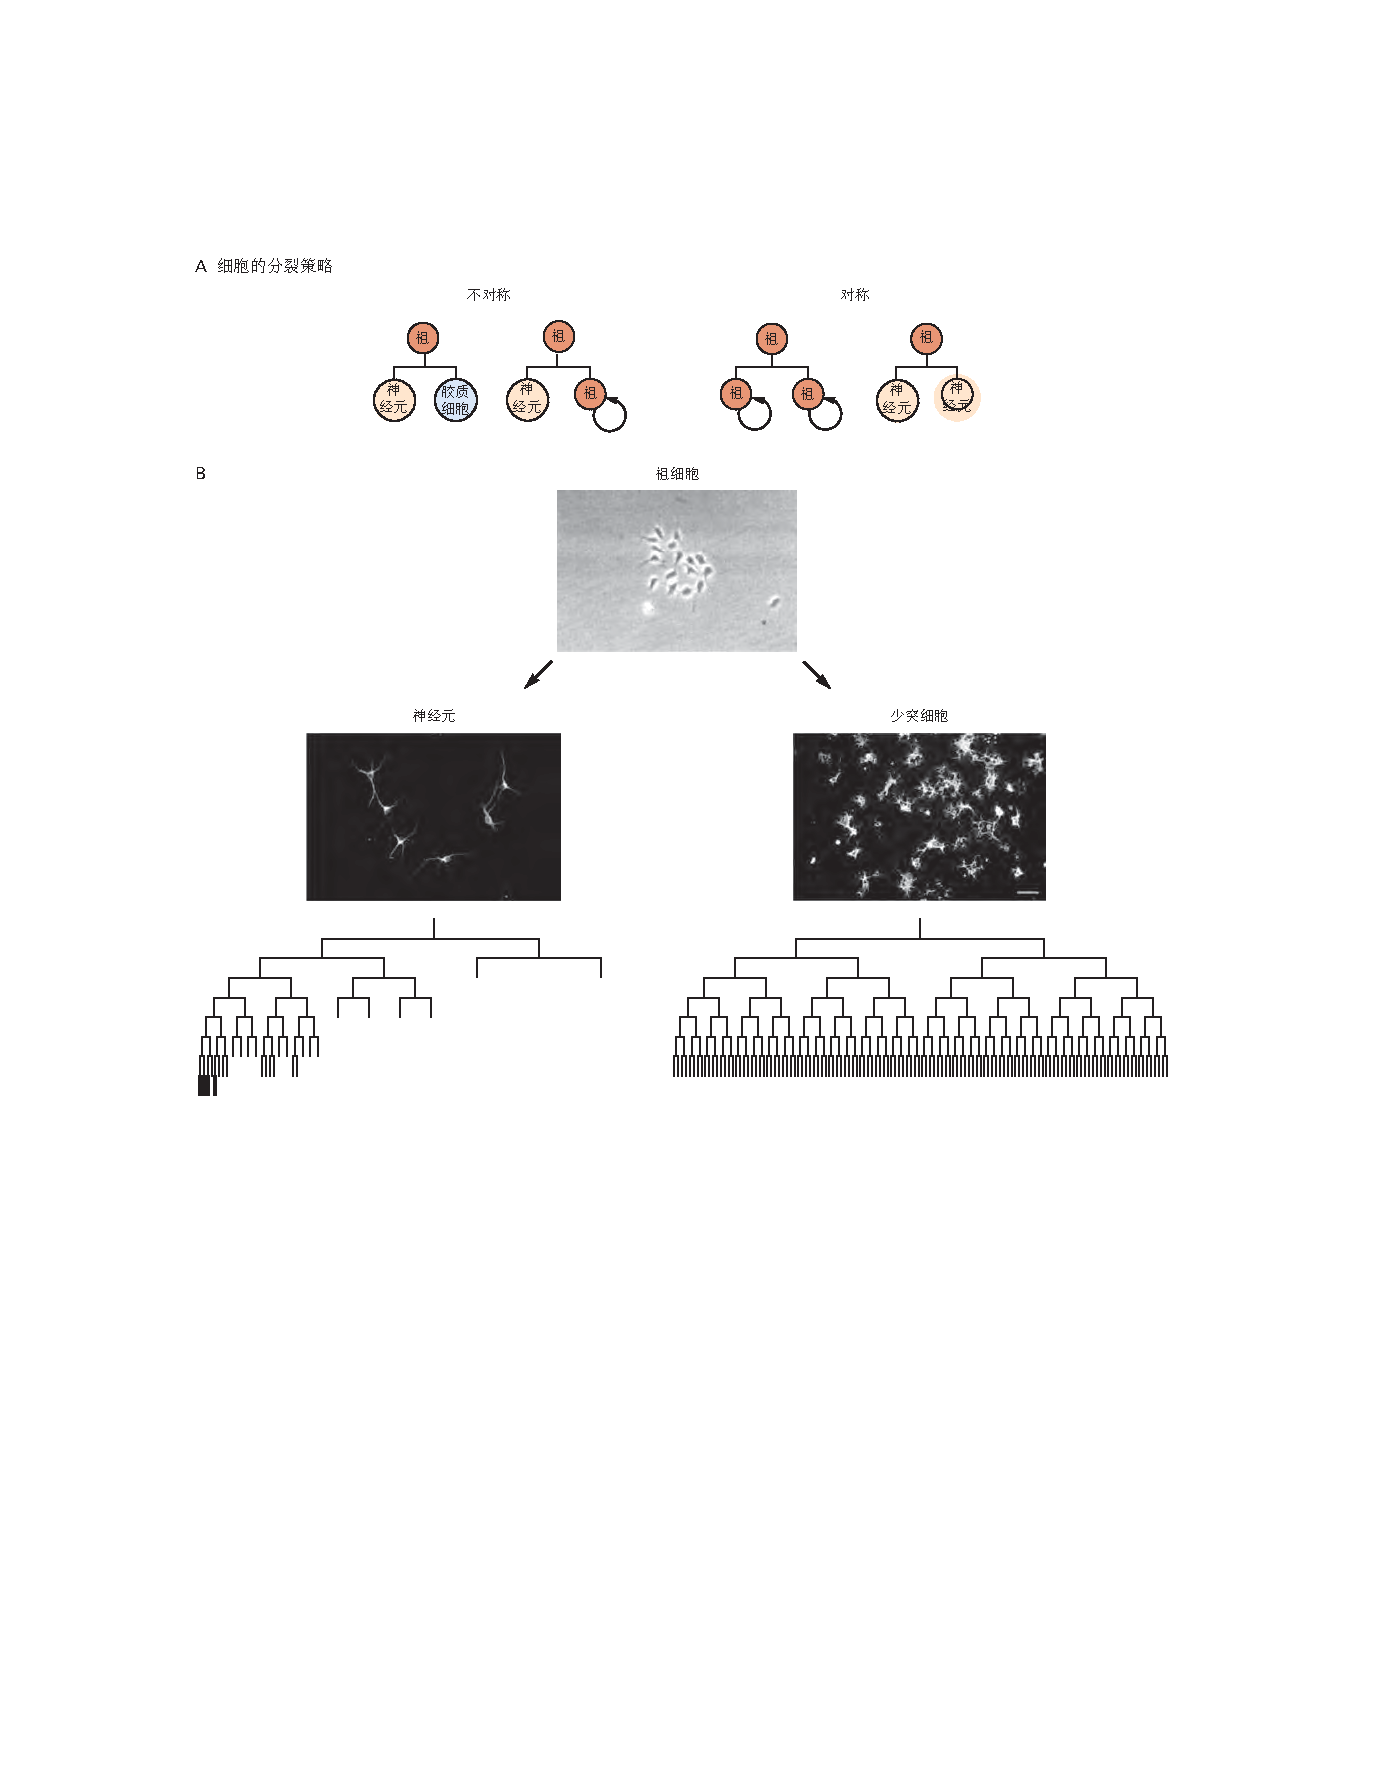
\includegraphics[width=1.0\linewidth]{chap46/fig_46_1}
	\caption{神经祖细胞具有不同的分裂模式。
		\textbf{A.} 细胞分裂的不对称和对称模式。
		\textit{祖细胞}可以进行不对称分裂以产生\textit{神经元}和神经\textit{胶质细胞},或\textit{神经元}和另一个\textit{祖细胞}。
		这种分裂模式有助于在发育早期产生神经元,在后期产生神经胶质细胞,这是中枢神经系统许多区域的典型特征。
		祖细胞也可以进行对称分裂以产生两个额外的祖细胞或两个有丝分裂后神经元。
		\textbf{B.} 延时摄影捕捉啮齿动物中分离的皮层祖细胞的分裂和分化。
		谱系图说明主要经历不对称分裂的细胞,产生神经元,或对称分裂,产生少突胶质细胞\cite{qian1998intrinsic}。}
	\label{fig:46_1}
\end{figure}


对称和不对称细胞分裂的发生率受分裂细胞局部环境中信号的影响,从而可以控制自我更新或分化的概率。
环境因素可以通过两种基本方式影响祖细胞分裂的结果。 它们可以以一种“指导性”的方式行事,使分裂过程的结果产生偏差,并导致干细胞以牺牲其他人为代价接受一种命运。
或者它们可以以“选择性”方式发挥作用,只允许某些细胞后代存活和成熟。



\section{放射状胶质细胞充当神经祖细胞和结构支架}

放射状神经胶质细胞是最早出现在原始神经上皮细胞内的形态学可区分的细胞类型。
它们的细胞体位于脑室区,长突延伸至软膜表面。
随着大脑变厚,放射状神经胶质细胞的突起仍然附着在脑室和软脑膜表面。
神经元生成完成后,许多放射状神经胶质细胞分化为星形胶质细胞。
径向神经胶质细胞的细长形状使其处于有利位置,可以作为从脑室区出现的神经元迁移的支架(图~\ref{fig:46_2})。


\begin{figure}[htbp]
	\centering
	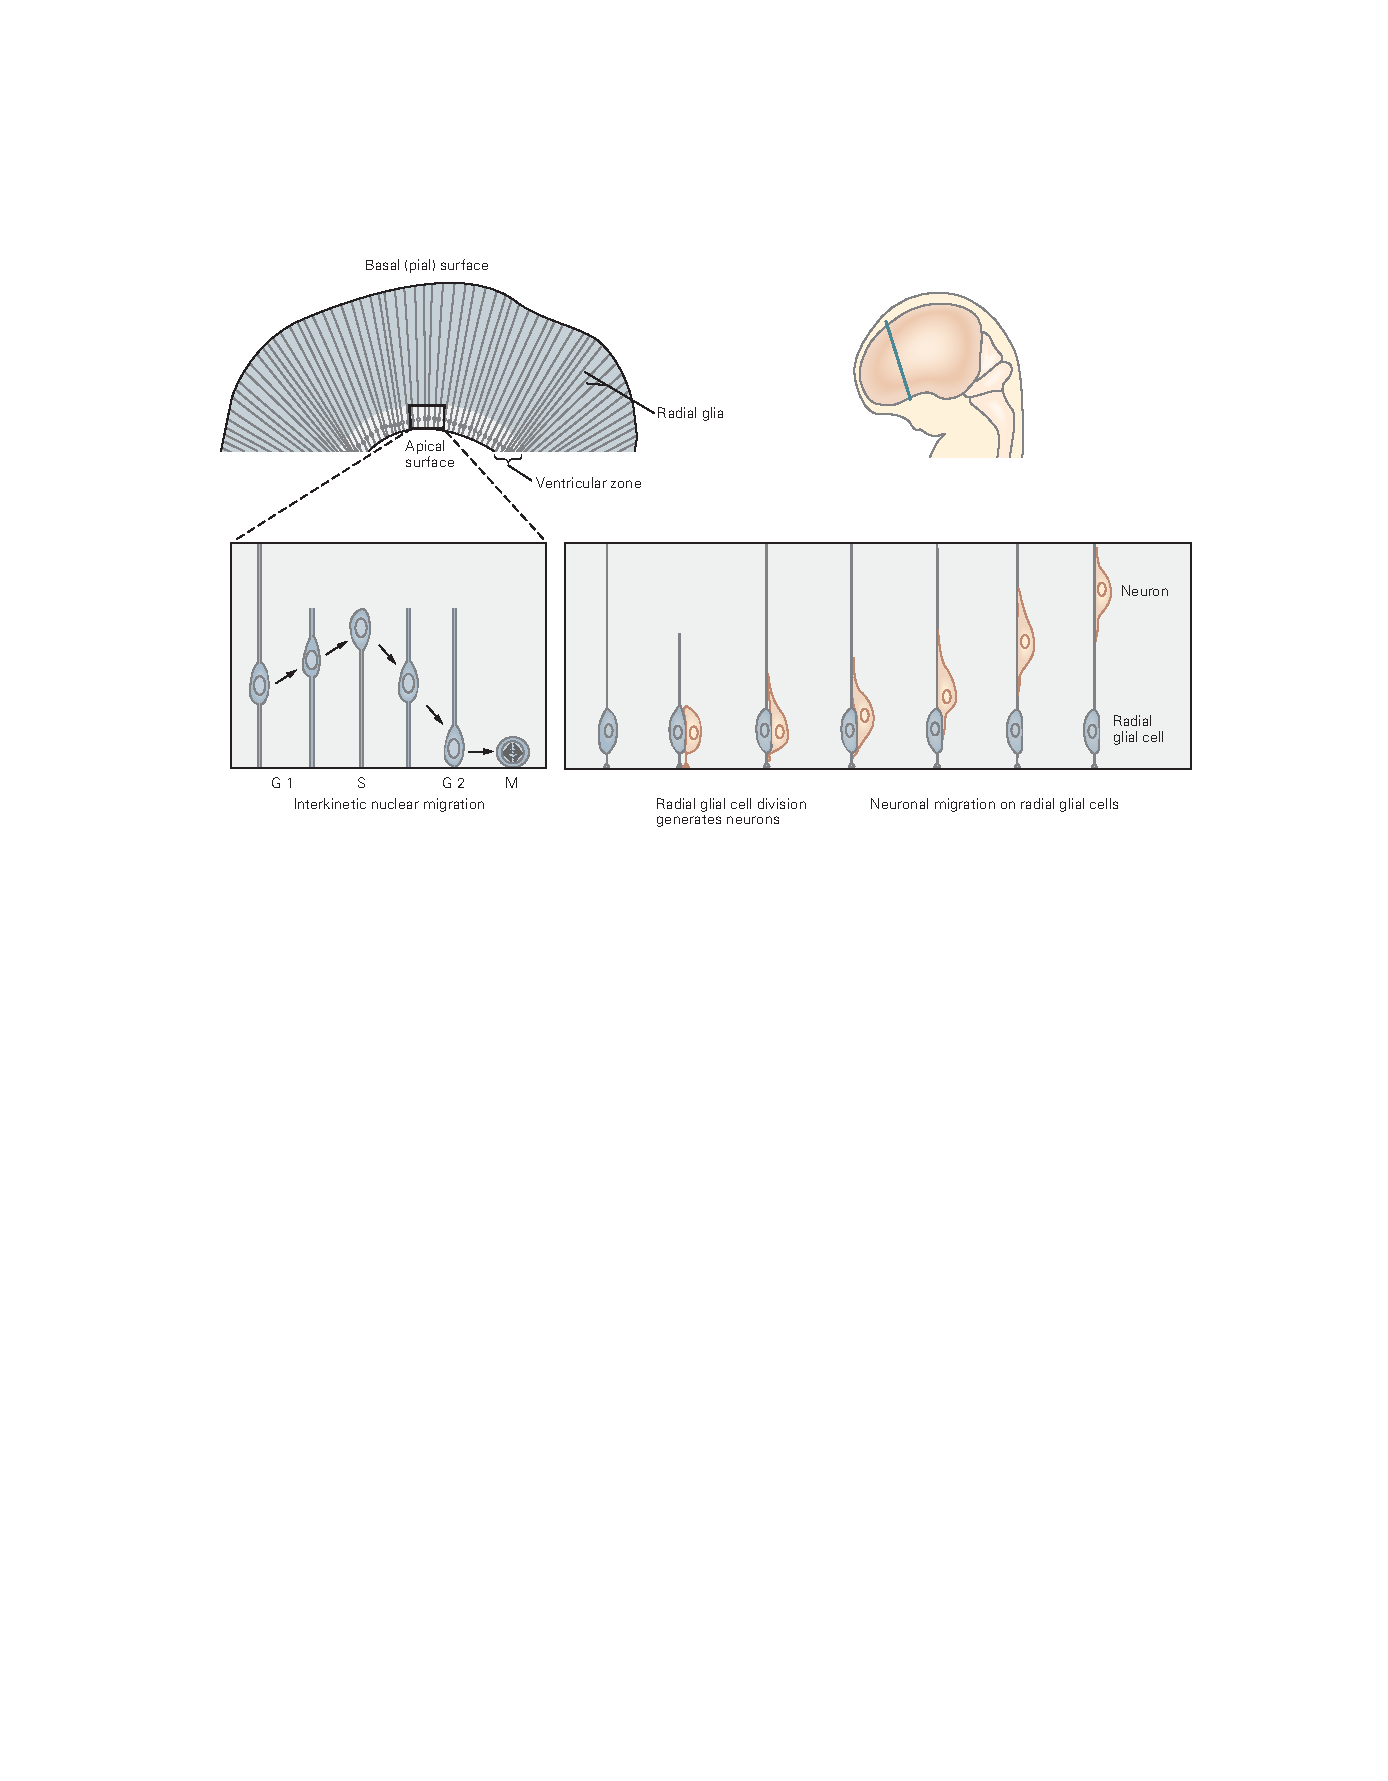
\includegraphics[width=1.0\linewidth]{chap46/fig_46_2}
	\caption{放射状胶质细胞作为中枢神经系统神经元的前体,也为放射状神经元迁移提供支架。
		发育中的大脑皮层脑室区祖细胞的细胞核随着细胞周期的进展沿顶端-基底轴迁移。
		左图:在 G1 期,细胞核从心室区的内(顶端)表面上升。
		在 S 期,它们位于心室区的外侧(基底)三分之一。
		在 G2 期,它们向顶端迁移,当细胞核到达心室表面时发生有丝分裂(M)。
		右图:在细胞分裂过程中,放射状神经胶质细胞产生有丝分裂后神经元,这些神经元以放射状神经胶质细胞为向导从心室区迁移出去。}
	\label{fig:46_2}
\end{figure}


心室区曾被认为包含两种主要细胞类型:
放射状神经胶质细胞和一组作为神经元主要来源的神经上皮祖细胞。
最近,这种经典观点发生了巨大变化。
一旦干细胞的对称分裂扩大了神经上皮细胞,这些细胞就会产生放射状神经胶质细胞。
放射状神经胶质细胞除了在神经元迁移中的作用外,还作为祖细胞产生神经元和星形胶质细胞(图~\ref{fig:46_2})。
用荧光染料或病毒标记放射状神经胶质细胞表明它们的克隆后代包括神经元细胞和放射状神经胶质细胞。
这些发现表明放射状神经胶质细胞能够进行不对称和自我更新的细胞分裂,并作为有丝分裂后神经元和星形胶质细胞的主要来源。



\section{神经元和神经胶质细胞的生成受 Delta-Notch 信号和基本螺旋-环-螺旋转录因子的调节}

放射状神经胶质细胞如何决定自我更新、产生神经元或产生成熟的星形胶质细胞?
这个问题的答案涉及一个进化上保守的信号系统。


在果蝇和脊椎动物中,神经命运由细胞表面信号系统调节,该系统由跨膜配体 Delta 及其受体 Notch 组成。
这种信号系统在果蝇的遗传研究中得到揭示。
神经元从更大的外胚层细胞群中出现,称为原神经区,所有这些细胞都有产生神经元的潜力。
然而在原神经区内,只有某些细胞形成神经元;
其他的变成表皮支持细胞。


Delta 和 Notch 最初由所有原神经细胞以相似水平表达(图~\ref{fig:46_3}A)。
然而,随着时间的推移,Notch 活动在一个细胞中增强并在其相邻细胞中受到抑制。
Notch 活性最高的细胞失去了形成神经元的潜力,并获得了另一种命运。
Delta 与 Notch 的结合导致 Notch 细胞质结构域的蛋白水解切割,然后进入细胞核。
在那里,它充当转录因子,调节\textit{碱性螺旋环螺旋}家族的其他转录因子级联的活性。
\textit{碱性螺旋环螺旋}转录因子抑制细胞成为神经元的能力并降低配体 Delta 的表达水平(图~\ref{fig:46_3}B、C)。


\begin{figure}[htbp]
	\centering
	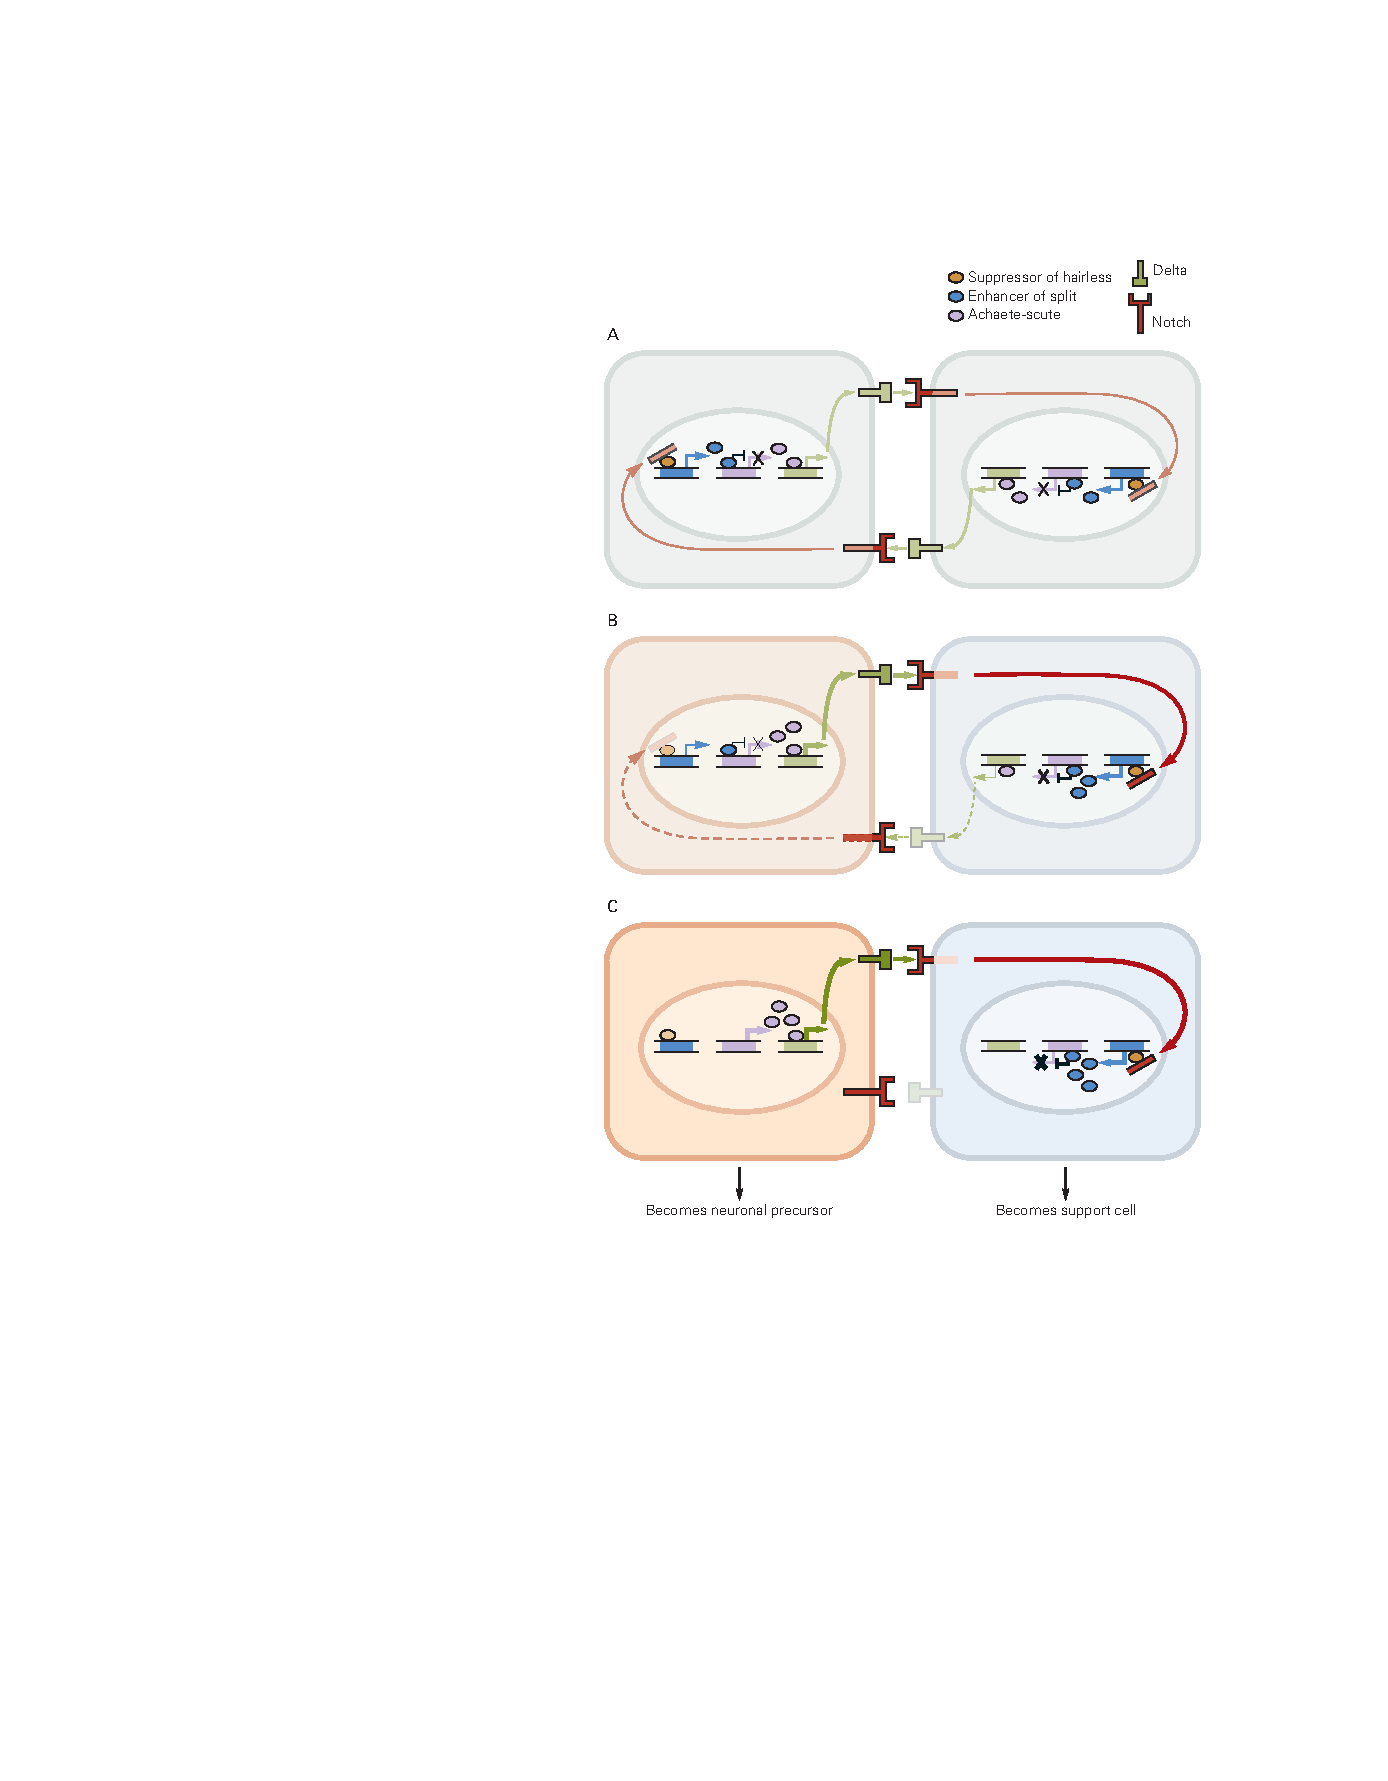
\includegraphics[width=0.75\linewidth]{chap46/fig_46_3}
	\caption{Delta 结合受体 Notch 并决定神经元的命运。
		\textbf{A.} 在两个细胞相互作用开始时,Delta 与受体 Notch 结合。
		Delta 和 Notch 在每个细胞中的表达水平相似,因此它们的初始信号强度相等。
		\textbf{B.} Delta-Notch 信号强度的微小失衡破坏了相互作用的对称性。
		在本例中,左侧细胞提供了稍大的 Delta 信号,从而更大程度地激活了右侧细胞中的 Notch 信号。
		在与 Delta 结合后,Notch 的细胞质结构域被切割形成称为 Notch-Intra 的蛋白水解片段,该片段进入细胞核并启动调节 Delta 表达水平的\textit{碱性螺旋环螺旋}转录级联。
		Notch-Intra 与\textit{碱性螺旋环螺旋}蛋白(无毛抑制因子)形成转录复合物,它结合并激活编码第二个\textit{碱性螺旋环螺旋}蛋白(分裂增强子)的基因。
		一旦被激活,分裂增强子就会结合并抑制编码第三种\textit{碱性螺旋环螺旋}蛋白 achaetescute 的基因的表达。
		Achaete-scute 活动促进 Delta 的表达。
		因此,通过抑制 achaete-scute,分裂增强子减少了 Delta 基因的转录激活和 Delta 蛋白的产生。
		这削弱了右侧细胞激活左侧细胞 Notch 信号的能力。
		\textbf{C.} 一旦左侧细胞中的 Notch 信号水平降低,无毛抑制因子不再激活分裂增强子,无毛壳细胞的表达水平增加,导致 Delta 表达增强,进一步激活 Notch 信号 正确的细胞。
		通过这种方式,Delta-Notch 信号中的一个小的初始不平衡被迅速放大为两个细胞中 Notch 激活水平的显著不对称。
		在哺乳动物中枢神经系统中,具有高水平 Notch 激活的细胞从神经元命运中转移,而具有低水平 Notch 激活的细胞成为神经元。}
	\label{fig:46_3}
\end{figure}


细胞间 Notch 水平的初始差异可能很小,在某些情况下是随机的(随机的)。
然而,通过这种反馈途径,这些最初的微小差异被放大,在 Notch 激活状态上产生全有或全无差异,从而影响两个细胞的命运。
Delta-Notch 和\textit{碱性螺旋环螺旋}信号的这种基本逻辑在脊椎动物和无脊椎动物的神经组织中得到保存。


Notch 信号如何调节哺乳动物的神经元和神经胶质细胞的产生?
在哺乳动物皮层发育的早期阶段,Notch 信号通过激活\textit{碱性螺旋环螺旋}转录抑制因子的 Hes 家族成员来促进放射状神经胶质细胞的生成。
其中两种蛋白质 Hes1 和 Hes5 似乎通过激活神经调节蛋白的 ErbB 类酪氨酸激酶受体的表达来维持放射状神经胶质细胞的特征,神经调节蛋白是一种促进放射状神经胶质细胞特性的分泌信号。
Notch 配体 Delta1 以及神经调节蛋白由新生成的皮层神经元表达;
因此,放射状神经胶质细胞依赖于来自其后代神经元的反馈信号来持续生产。


在皮层发育的后期阶段,Notch 信号继续激活 Hes 蛋白,但细胞内反应途径的变化导致星形胶质细胞分化。
在这个阶段,Hes 蛋白通过激活转录因子 STAT3 发挥作用,STAT3 招募丝氨酸-苏氨酸激酶 JAK2,这是一种有效的星形胶质细胞分化诱导剂。
STAT3 还激活星形胶质细胞特异性基因的表达,例如神经\textit{胶质纤维酸性蛋白}。


少突胶质细胞(中枢神经系统中第二大类神经胶质细胞)的产生遵循许多控制神经元和星形胶质细胞生成的原则(图~\ref{fig:46_4})。
Notch 信号调节两个\textit{碱性螺旋环螺旋}转录因子 Olig1 和 Olig2 的表达,它们在胚胎和出生后少突胶质细胞的产生中具有重要作用。


\begin{figure}[htbp]
	\centering
	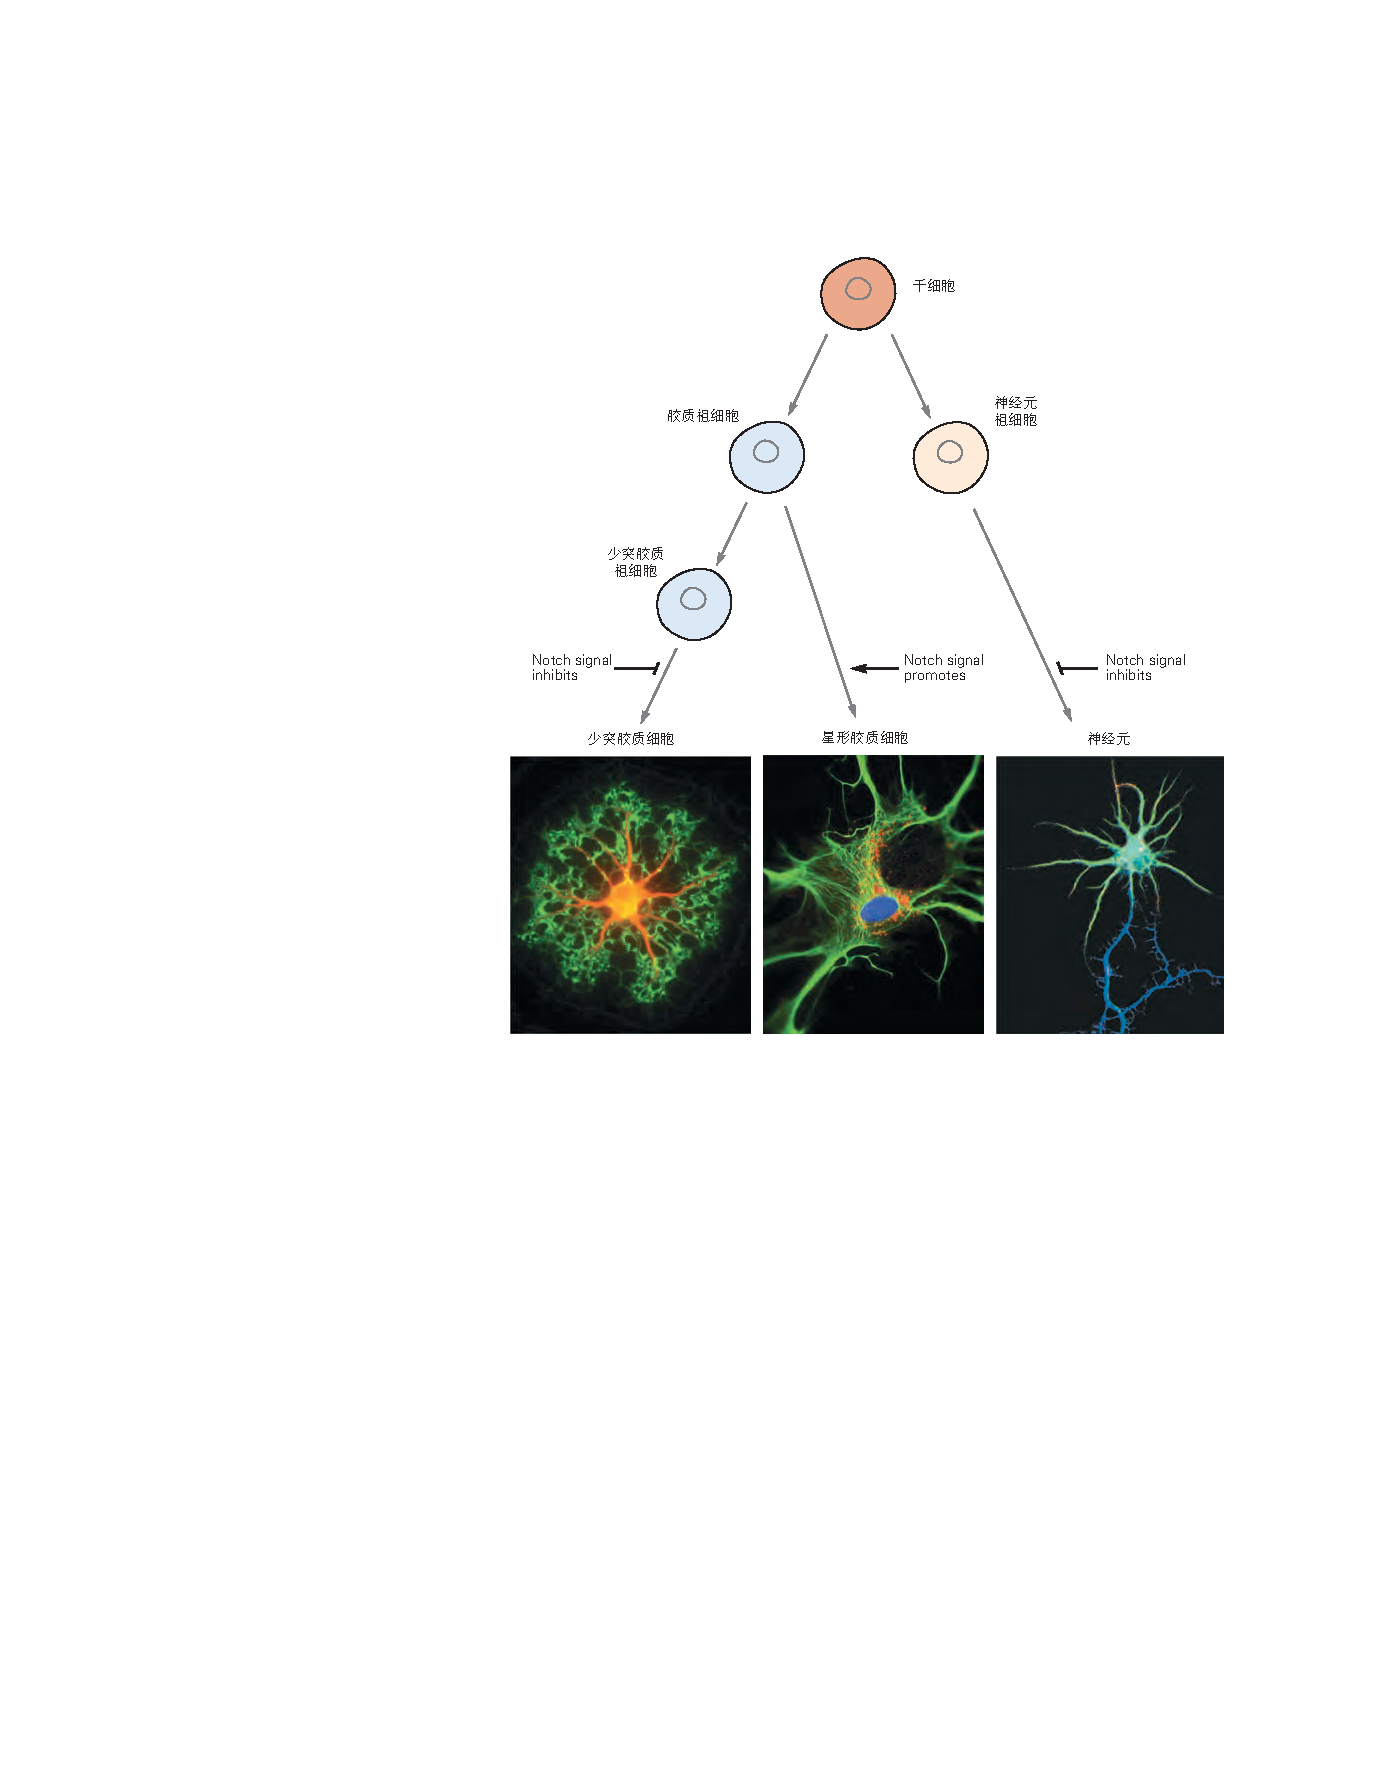
\includegraphics[width=0.85\linewidth]{chap46/fig_46_4}
	\caption{Notch 信号调节大脑皮层发育中细胞的命运。
		Notch 信号在发育中的大脑皮层的细胞分化中具有多种作用。
		神经胶质祖细胞中 Notch 信号的激活导致细胞分化为星形胶质细胞并抑制分化为少突胶质细胞(左通路)。
		Notch 信号还抑制祖细胞分化为神经元(右通路)。}
	\label{fig:46_4}
\end{figure}


存在其他机制以确保在注定要成为神经元的细胞中避免 Notch 信号的影响。
一个涉及称为 Numb 的细胞质蛋白。
Numb 在神经发生中的关键作用首先在果蝇中得到证实,它决定了不对称分裂祖细胞的子细胞的神经元命运。
在哺乳动物皮层中,Numb 优先定位于神经元子细胞并拮抗 Notch 信号传导。
Numb 活性的丧失导致祖细胞大量增殖。
Notch 信号传导的抑制导致几种原神经\textit{碱性螺旋环螺旋}转录因子的表达,特别是 Mash1、neurogenin-1 和 neurogenin-2。
Neurogenins 通过激活下游\textit{碱性螺旋环螺旋}蛋白(如 neuroD)来促进神经元的产生,并且它们通过抑制 JAK 和 STAT 信号传导来阻止星形胶质细胞的形成。


尽管 Delta-Notch 信号和\textit{碱性螺旋环螺旋}转录因子激活剂是决定产生神经元或神经胶质细胞的核心,但一些额外的转录途径增强了这一核心分子程序。
一种重要的转录因子 REST/NRSF 抑制神经祖细胞和神经胶质细胞中神经元基因的表达。
REST/NRSF 随着神经元分化而迅速降解,从而允许神经源性\textit{碱性螺旋环螺旋}因子和其他神经元基因的表达。
SoxB 类的同源域转录因子也通过阻断神经源性\textit{碱性螺旋环螺旋}蛋白活性在维持神经祖细胞中发挥重要作用。
因此,神经元的分化需要避免 REST/NRSF 和 SoxB 蛋白活性。



\section{大脑皮层的层数是通过新生神经元的顺序添加而建立的}

哺乳动物神经管最前部的脑室区通过一系列步骤产生大脑皮层。
位于神经上皮顶端边缘的脑室区的细胞最初向基底部迁移形成脑室下区,其中包含一组命运更受限制的祖细胞。
形成旁边是一个中间区,新形成的神经元通过它迁移,还有一个预板,它容纳最早出生的神经元。
额外的神经元迁移形成位于前板内的称为皮层板的层。 
因此,皮层板将前板分为顶端亚板和基底边缘区(图~\ref{fig:46_5}A)。


\begin{figure}[htbp]
	\centering
	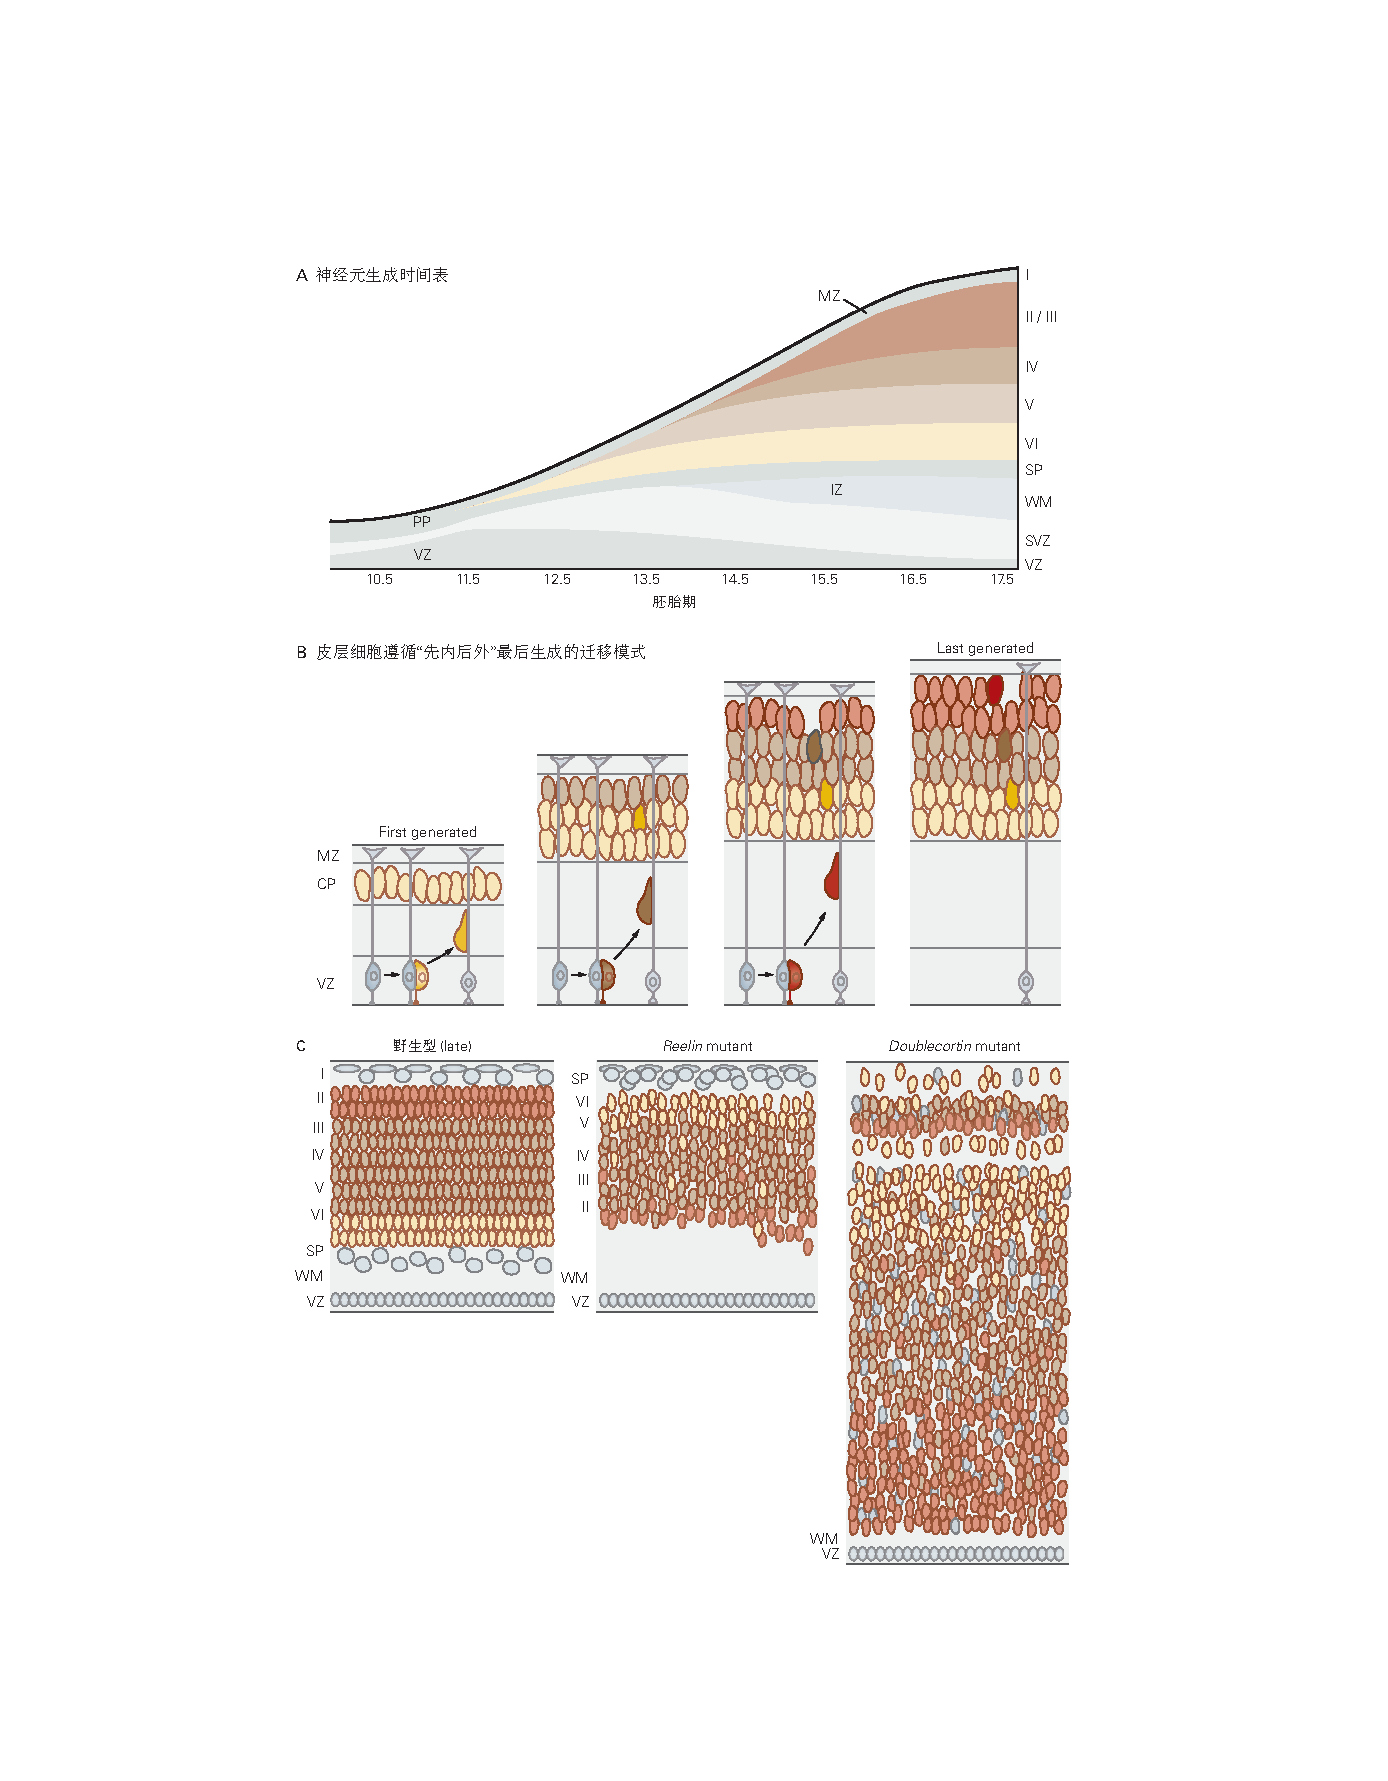
\includegraphics[width=0.79\linewidth]{chap46/fig_46_5}
	\caption{胚胎大脑皮层内神经元的迁移导致分层皮层组织\cite{olson2002smooth}。
		\textbf{A.} 这种神经发生的时间顺序适用于小鼠大脑皮层。
		在胚胎发育的最后 5 天,神经元开始在皮层板中积累。
		在皮层板内,神经元在进入表层之前填充在深层。 
		\textbf{B.} 在正常皮层发育过程中,神经元使用放射状神经胶质细胞作为迁移支架进入皮层板。
		当它们接近软膜表面时,神经元停止迁移并从放射状神经胶质细胞中分离出来。
		这种有序的神经元迁移模式导致成熟大脑皮层中形成六个神经元层,排列在白质和亚板之间。
		\textbf{C.} 在缺乏功能性卷轴蛋白的小鼠突变卷轴器中,皮层板中神经元的分层被严重破坏并部分倒置。
		此外,整个皮层板在亚板下方发育。
		在双皮层突变体中,皮层变厚,神经元失去其特征性的分层特性,并且某些层包含更少的神经元。
		在 Lis1 突变体中观察到类似的破坏,这是某些形式的人类无脑畸形的基础。}
	\label{fig:46_5}
\end{figure}


一旦进入皮层板,神经元就会组织成明确的层。
神经元所在的层与神经元的生日精确相关,这个术语指的是分裂的前体细胞经历最后一轮细胞分裂并产生有丝分裂后神经元的时间。
从脑室和脑室下区迁移并在早期阶段离开细胞周期的细胞会产生定居在皮层最深层的神经元。
在逐渐晚些阶段退出细胞周期的细胞迁移更长的距离并通过较早出生的神经元,然后定居在皮层的更表层。
因此,大脑皮层中神经元的分层遵循先内后外的规则(图~\ref{fig:46_5}B)。



\section{神经元从它们的起源位置长距离迁移到它们的最终位置}

神经元从皮层脑室区向皮层板的迁移遵循称为径向迁移的过程。
在这种模式下,神经元沿着放射状神经胶质细胞的长而无分支的过程移动以到达它们的目的地。
相反,中间神经元通过称为切向迁移的过程从皮层下位点进入皮层。
我们依次讨论这些模式,然后描述第三种迁移策略,自由迁移,它在周围神经系统中占主导地位。



\subsection{兴奋性皮层神经元沿神经胶质指南径向迁移}

1970 年代皮层发育的经典解剖学研究提供的证据表明,在心室区产生的神经元沿着放射状神经胶质纤维的通路迁移到它们的固定位置。
放射状神经胶质细胞作为放射状神经元迁移的主要支架。
它们的细胞体靠近脑室表面,产生横跨发育中脑壁宽度的细长纤维。
每个放射状神经胶质细胞在脑室区的顶面都有一个基底端足,并在软脑膜表面有多个端足终止(图~\ref{fig:46_6})。
放射状神经胶质支架在灵长类动物皮层的发育中尤为重要,随着皮层的扩张,神经元需要长距离迁移。
在最终分化为星形胶质细胞之前,单个放射状神经胶质细胞支架可以支持多达 30 代的皮层神经元迁移。


\begin{figure}[htbp]
	\centering
	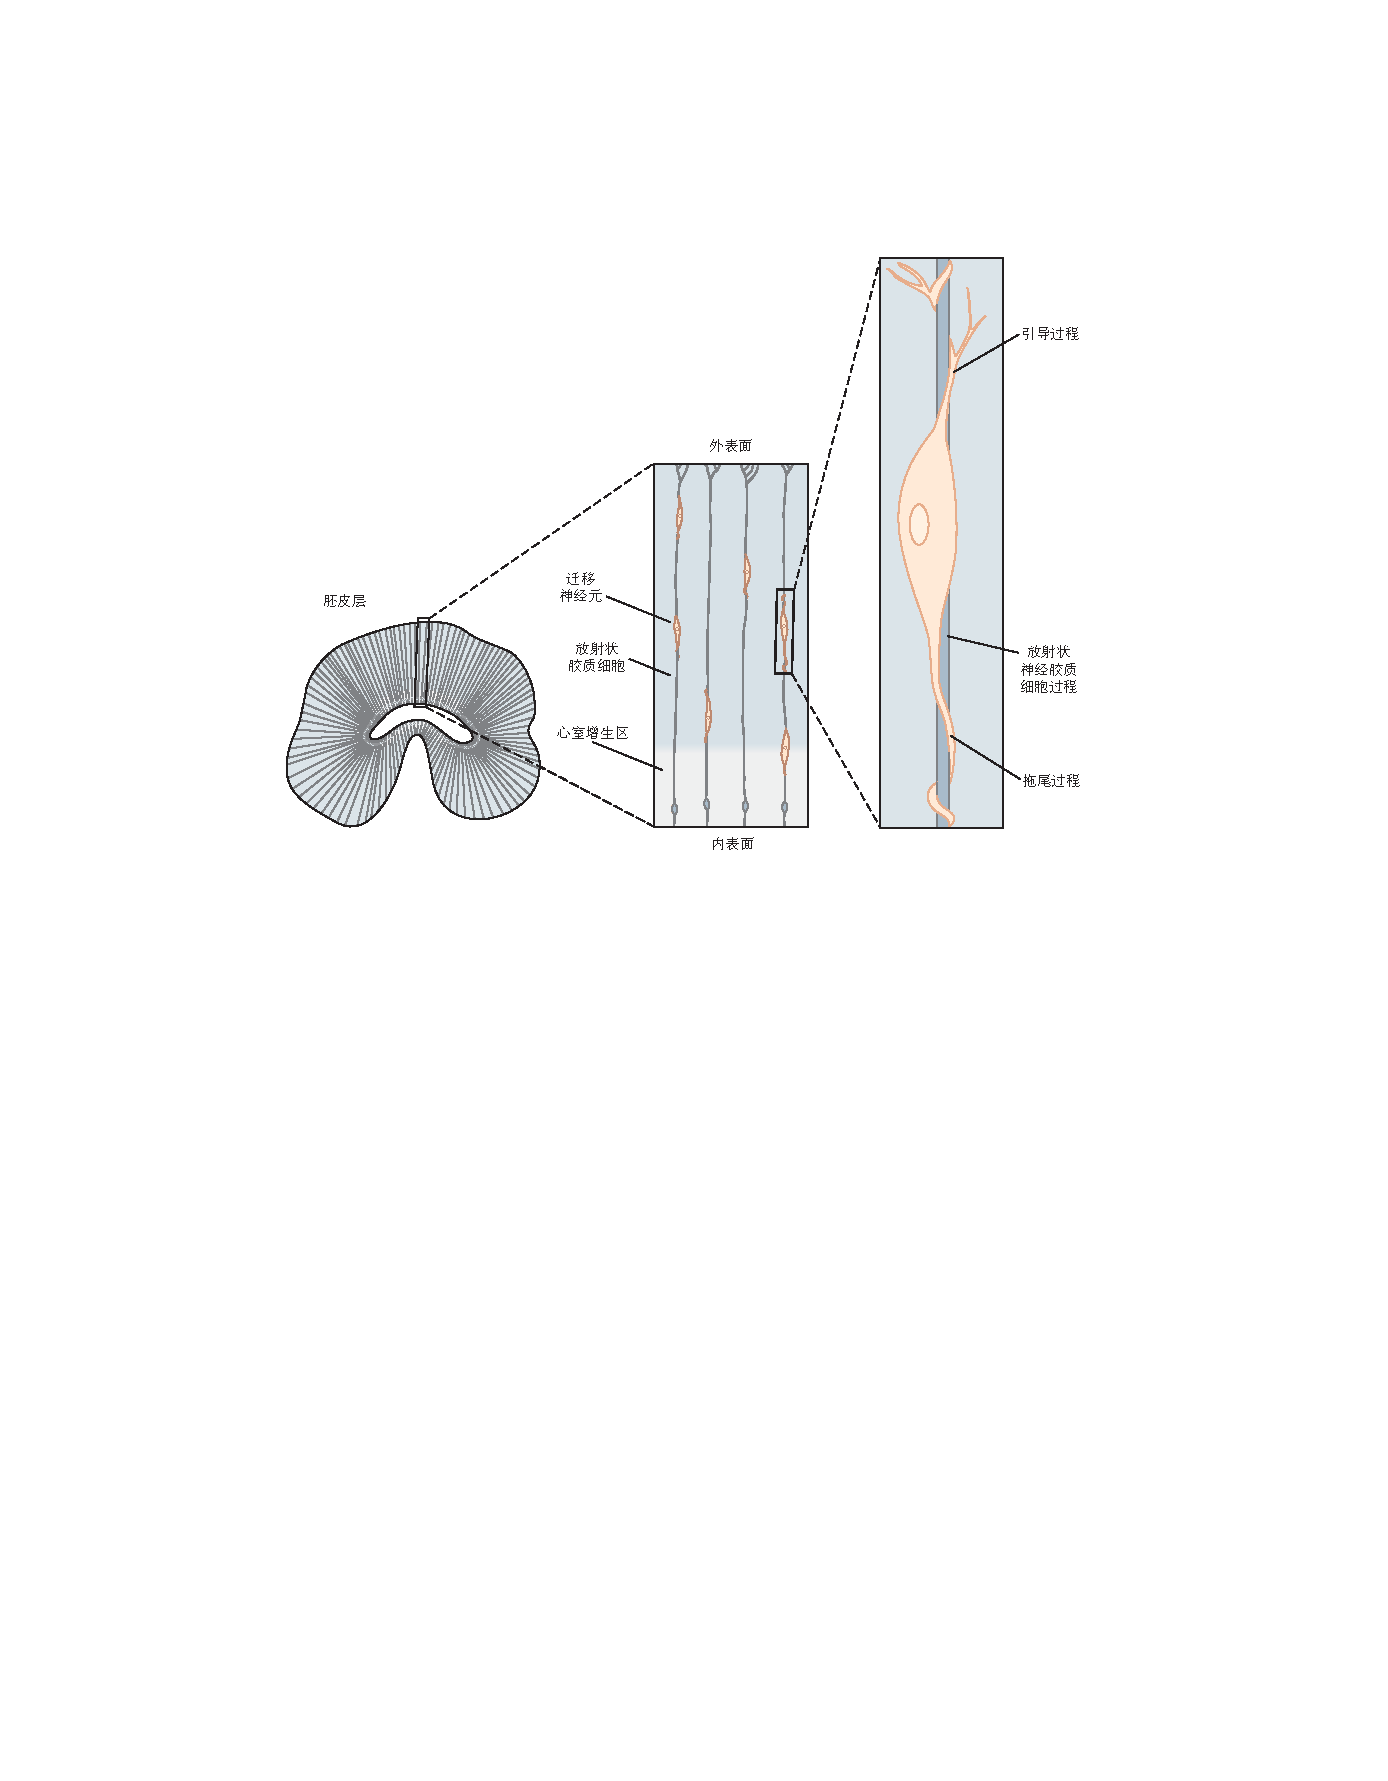
\includegraphics[width=1.0\linewidth]{chap46/fig_46_6}
	\caption{神经元沿着放射状神经胶质细胞迁移。
		在从放射状胶质细胞生成后,胚胎大脑皮层中新产生的神经元延伸了一个围绕放射状胶质细胞轴的主导过程,因此在它们从脑室区迁移到软脑膜表面的过程中使用放射状胶质细胞作为支架皮层。}
	\label{fig:46_6}
\end{figure}


是什么力和分子为放射状神经胶质细胞的神经元迁移提供动力?
神经元离开细胞周期后,其前导突缠绕在放射状神经胶质细胞的轴周围,其细胞核在前导突的细胞质内易位。
尽管迁移神经元的主导过程缓慢而稳定地延伸,但由于细胞骨架的复杂重排,细胞核以间歇、逐步的方式移动。 
微管状晶格在细胞核周围形成一个笼子;
细胞核的运动依赖于称为基体的中心体样结构,微管系统从基体投射到主导过程中,提供细胞核移动的轨道(图~\ref{fig:46_7}A)。


\begin{figure}[htbp]
	\centering
	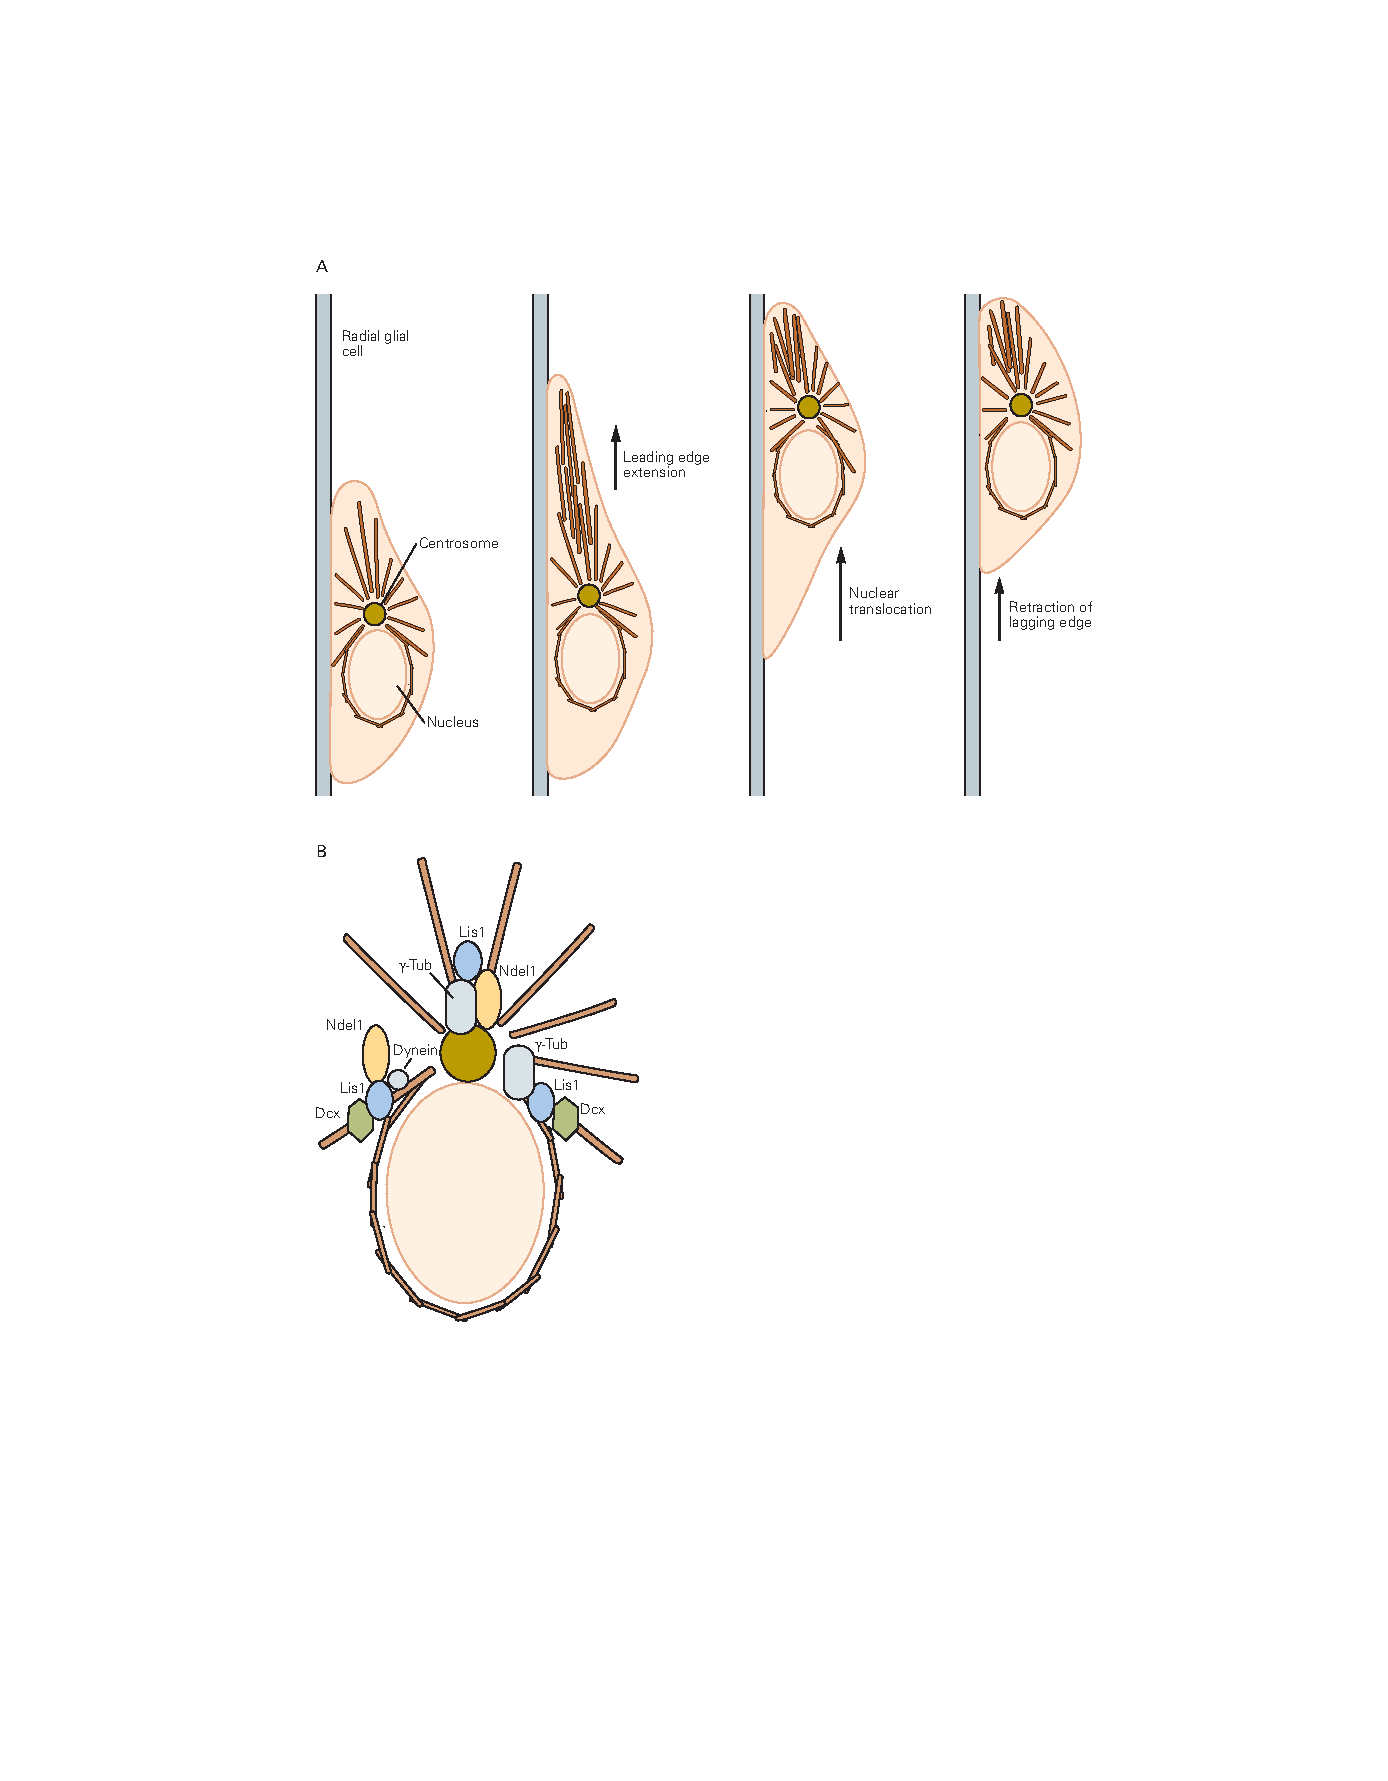
\includegraphics[width=1.0\linewidth]{chap46/fig_46_7}
	\caption{细胞骨架蛋白为神经元沿放射状神经胶质细胞的迁移提供动力。
		\textbf{A.} 微管细胞骨架在神经元迁移中具有重要作用。
		微管将细胞核包裹在笼状结构中。
		在有吸引力和排斥性的细胞外引导信号的控制下,沿径向神经胶质细胞的迁移涉及神经元在运动方向上的前导过程的延长。
		这些线索调节微管相关蛋白 Ndel1 和 Lis1(动力蛋白运动复合体的两个组分)和\textit{双皮质素}的磷酸化状态,它们共同稳定微管细胞骨架\cite{gleeson2000neuronal}。
		\textbf{B.} 微管通过一系列蛋白质附着在中心体上,这些蛋白质是神经元迁移障碍的破坏目标。}
	\label{fig:46_7}
\end{figure}


沿放射状胶质细胞的神经元迁移也涉及细胞之间的粘附相互作用。
诸如整合素的粘附受体促进放射状神经胶质细胞上的神经元延伸。
然而,神经元沿神经胶质纤维的迁移不同于生长锥驱动的轴突的延伸(第~\ref{chap:chap47}~章)。
在神经元迁移中,主导过程缺乏代表生长锥的结构化肌动蛋白丝,更类似于延伸的树突,这是\textit{圣地亚哥$\cdot$拉蒙-卡哈尔}首先做出的推论。


皮层神经元迁移和定居程序的中断是许多人类皮层病理学的基础(图~\ref{fig:46_5}C)。
例如,在无脑畸形(希腊语,光滑脑,指的是患有这种疾病的患者皮层表面的特征性平滑)中,神经元离开脑室区但未能完成向皮层板的迁移。
结果,成熟的皮层通常从六个神经元层减少到四个神经元层,并且每个剩余层中的神经元排列是无序的。
偶尔,无脑畸形伴随着皮层下白质中存在一组额外的神经元。
Lis1 和\textit{双皮质素}基因突变导致的无脑畸形患者通常患有严重的智力障碍和顽固性癫痫。
Lis1 和\textit{双皮质素}蛋白定位于微管,这表明它们参与了微管依赖性核运动,尽管它们在神经元迁移中的确切功能仍不清楚。


破坏\textit{络丝蛋白}信号通路的突变会破坏神经元迁移通过皮层亚板的最后阶段。
卷轴蛋白由\textit{卡-雷氏细胞}分泌,\textit{卡-雷氏细胞}是在前板和边缘区发现的一类神经元。
来自这些细胞的信号对于皮层神经元的迁移至关重要。
在缺乏功能性\textit{络丝蛋白}的小鼠中,神经元无法从其放射状神经胶质支架上分离并堆积在皮层板下方,这违反了由内向外的迁移规则。
结果,细胞类型的正常分层被部分反转并且边缘区丢失。
\textit{络丝蛋白}通过细胞表面受体起作用,包括 ApoE 受体 2 和极低密度脂蛋白受体。
\textit{络丝蛋白}与这些受体的结合会激活细胞内蛋白 Dab1,该蛋白可转导\textit{络丝蛋白}信号。
毫不奇怪,转导卷轴蛋白信号的蛋白质丢失会产生类似的迁移表型。



\subsection{皮层中间神经元在皮层下出现并切向迁移到皮层}

皮层心室区的祖细胞最初被认为会产生所有皮层神经元。
然而,随着针对不同神经元类型的更好分子标记的出现,人们发现中间神经元出现在皮层下结构的脑室区。
它们中的大多数起源于称为神经节隆起的腹侧端脑区域(图~\ref{fig:46_8})。


\begin{figure}[htbp]
	\centering
	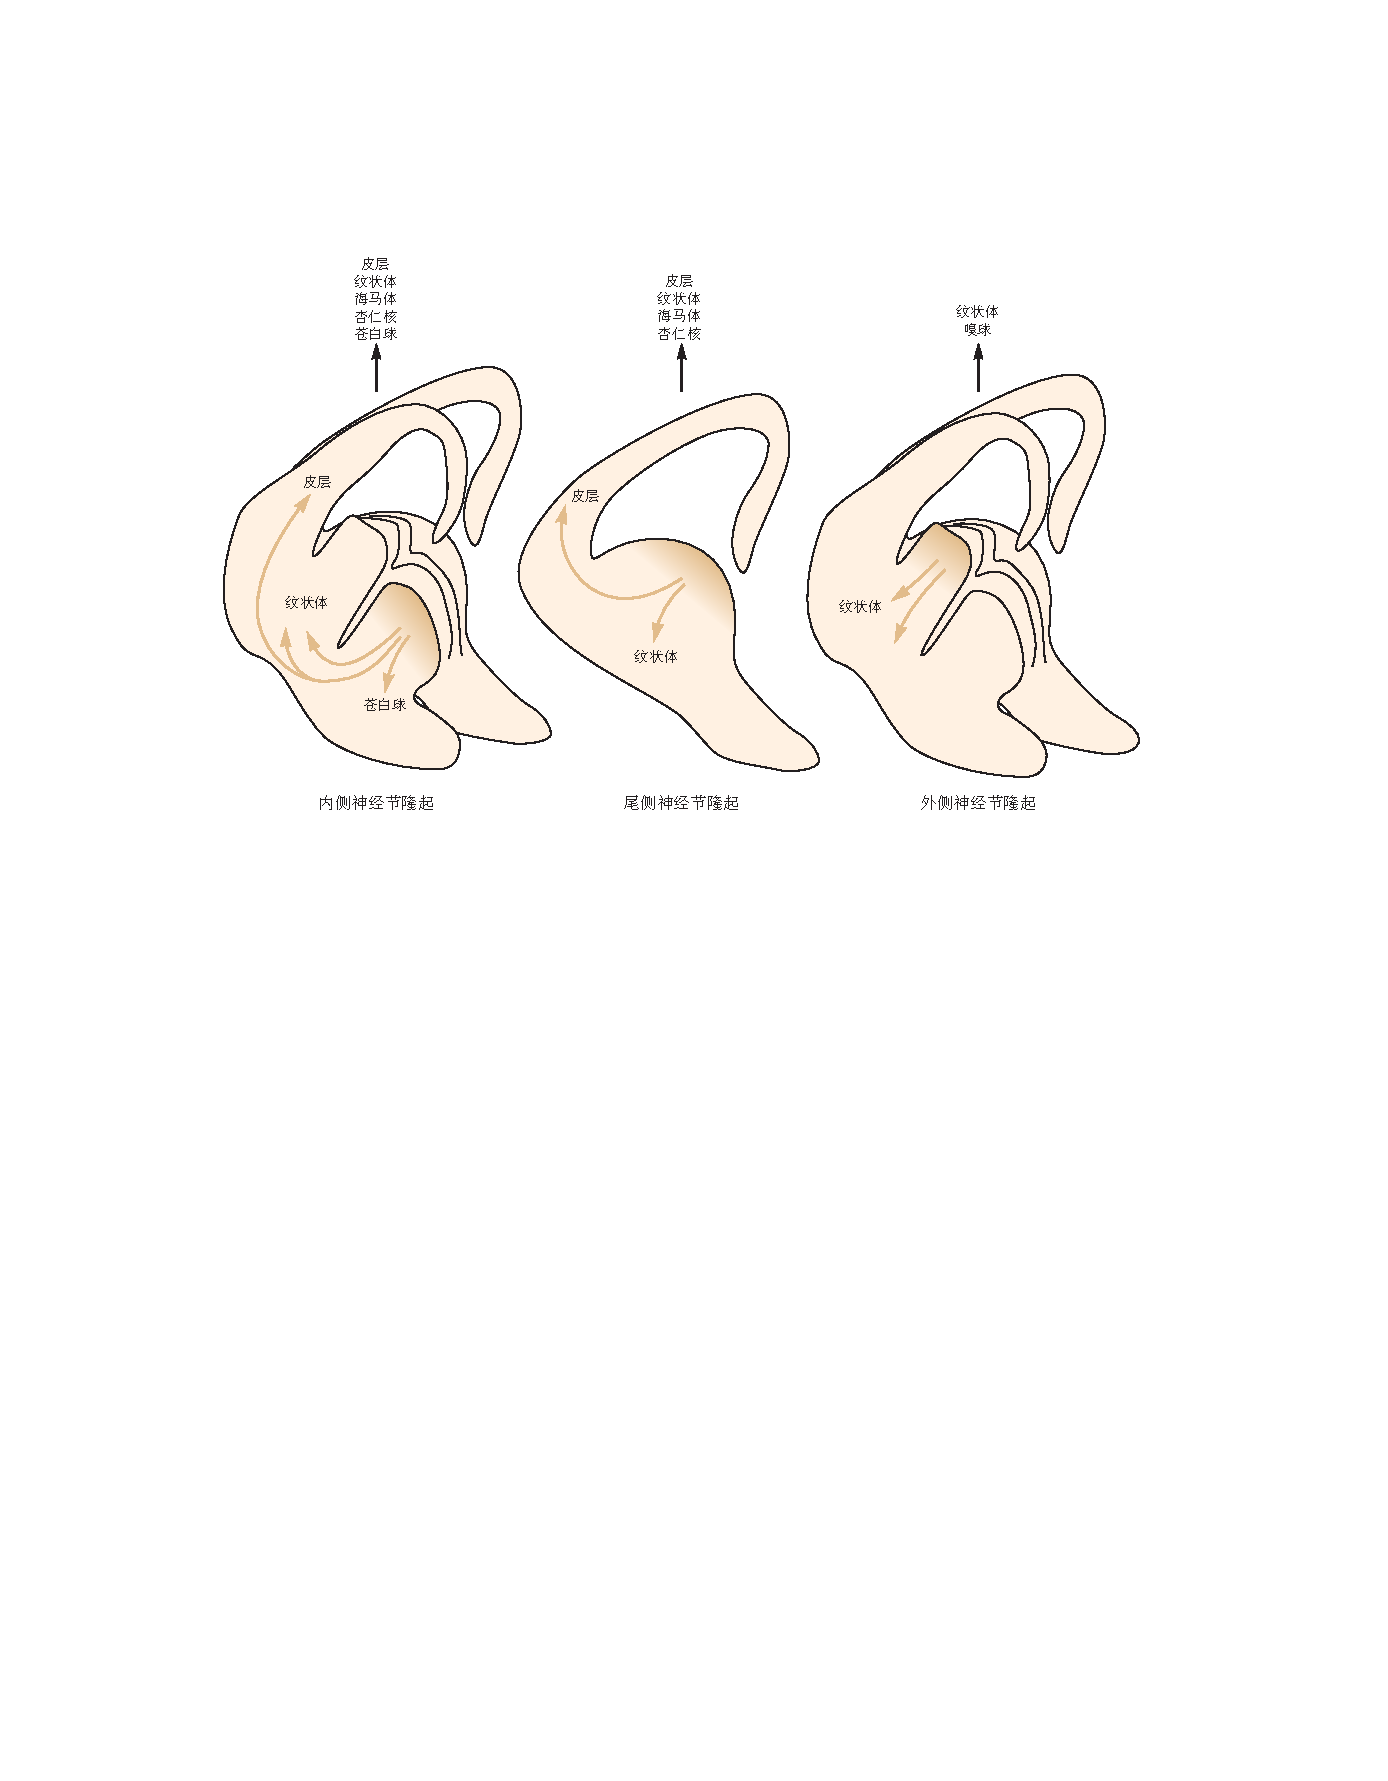
\includegraphics[width=1.0\linewidth]{chap46/fig_46_8}
	\caption{前脑中间神经元在腹侧端脑中产生,并切向迁移到大脑皮层。
		在神经节隆突中产生的神经元迁移到前脑的许多区域并定居,在那里它们分化为中间神经元。
		皮层中间神经元起源于内侧和尾部神经节隆起。
		在这些区域产生的其他细胞向其他方向迁移,在海马体、纹状体、苍白球和杏仁核中填充中间神经元。
		外侧神经节隆起产生迁移到纹状体和嗅球的细胞。
		迁移到灯泡的细胞使用相邻的迁移细胞作为迁移的底物,这一过程称为链迁移\cite{bandler2017cortical}。}
	\label{fig:46_8}
\end{figure}


内侧和中央隆起产生大部分皮层中间神经元,这些神经元从它们的起源部位向背侧迁移进入皮层。
一些通过中间区域进入,而另一些则通过边缘区域进入(图~\ref{fig:46_5}A)。
一旦它们到达特定的前后和中间位置,它们就会切换到径向迁移模式,以行进最终距离到适当的层。
神经节隆突中产生的不同神经元群在不同时间通过不同途径迁移,从而导致神经元间群的多样性。
时间和起源地、迁徙路线和最终命运之间的精确关系仍有待确定。
尽管如此,现在很清楚皮层神经元有两个来源:来自皮层心室区的兴奋性神经元和来自神经节隆起的中间神经元。


其他前脑结构中的中间神经元也来自神经节隆起,以及一些其他皮层下部位,例如视前区。
从内侧和尾部突起向尾部迁移的细胞填充海马体,而从这些区域腹侧迁移的细胞填充基底神经节。
相比之下,在外侧神经节隆起中产生的神经元向嘴侧迁移并贡献嗅球的球周和颗粒中间神经元。
在这个喙迁移流中,神经元使用相邻的神经元作为迁移(链迁移)的底物。
在成年大脑中,跟随延髓迁移流的神经元起源于纹状体的脑室下区。


转录因子控制神经节隆起神经元的特性。
同源结构域蛋白 Dlx1 和 Dlx2 由神经节隆突中的细胞表达。
在缺乏 Dlx1 和 Dlx2 活性的小鼠中,由此产生的神经元迁移扰动导致皮层中\textit{$\gamma$-氨基丁酸能}中间神经元数量大幅减少。
其他转录因子是造成神经节隆突之间差异的原因。
例如,Nkx2.1 由内侧神经节隆起的细胞选择性表达。
在它不存在的情况下,在该区域产生的中间神经元具有通常在外侧和尾部神经节隆起中产生的特征。
还有其他转录因子指定每个神经节隆突内神经元亚群的不同特征。


这些转录因子指定的主要特征之一是新生中间神经元采取的迁移路径。
由神经节隆起内和附近的细胞产生的大量可溶性和细胞表面因子提供了排斥性信号,导致细胞从心室区排出,所谓的促动(运动促进)信号加速了它们的迁移,而有吸引力的信号直接 他们到他们的目标。
这些因子包括狭缝、信号蛋白和肝配蛋白,我们将在第~\ref{chap:chap47}~章中遇到所有这些作为引导轴突到达其目标的分子。



\subsection{周围神经系统中的神经嵴细胞迁移不依赖于支架}

周围神经系统来源于神经嵴干细胞,神经管和表皮外胚层交界处的一小群神经上皮细胞。
诱导后不久,神经嵴细胞从上皮细胞转变为间充质细胞,并开始与神经管分离。
然后它们迁移到全身的许多部位(图~\ref{fig:46_9})。
神经嵴细胞迁移不依赖于支架(即放射状神经胶质细胞或预先存在的轴突束),因此称为自由迁移。
这种形式的神经元迁移需要显著的细胞结构和细胞粘附变化,并且不同于中枢神经系统中的大多数迁移事件。


\begin{figure}[htbp]
	\centering
	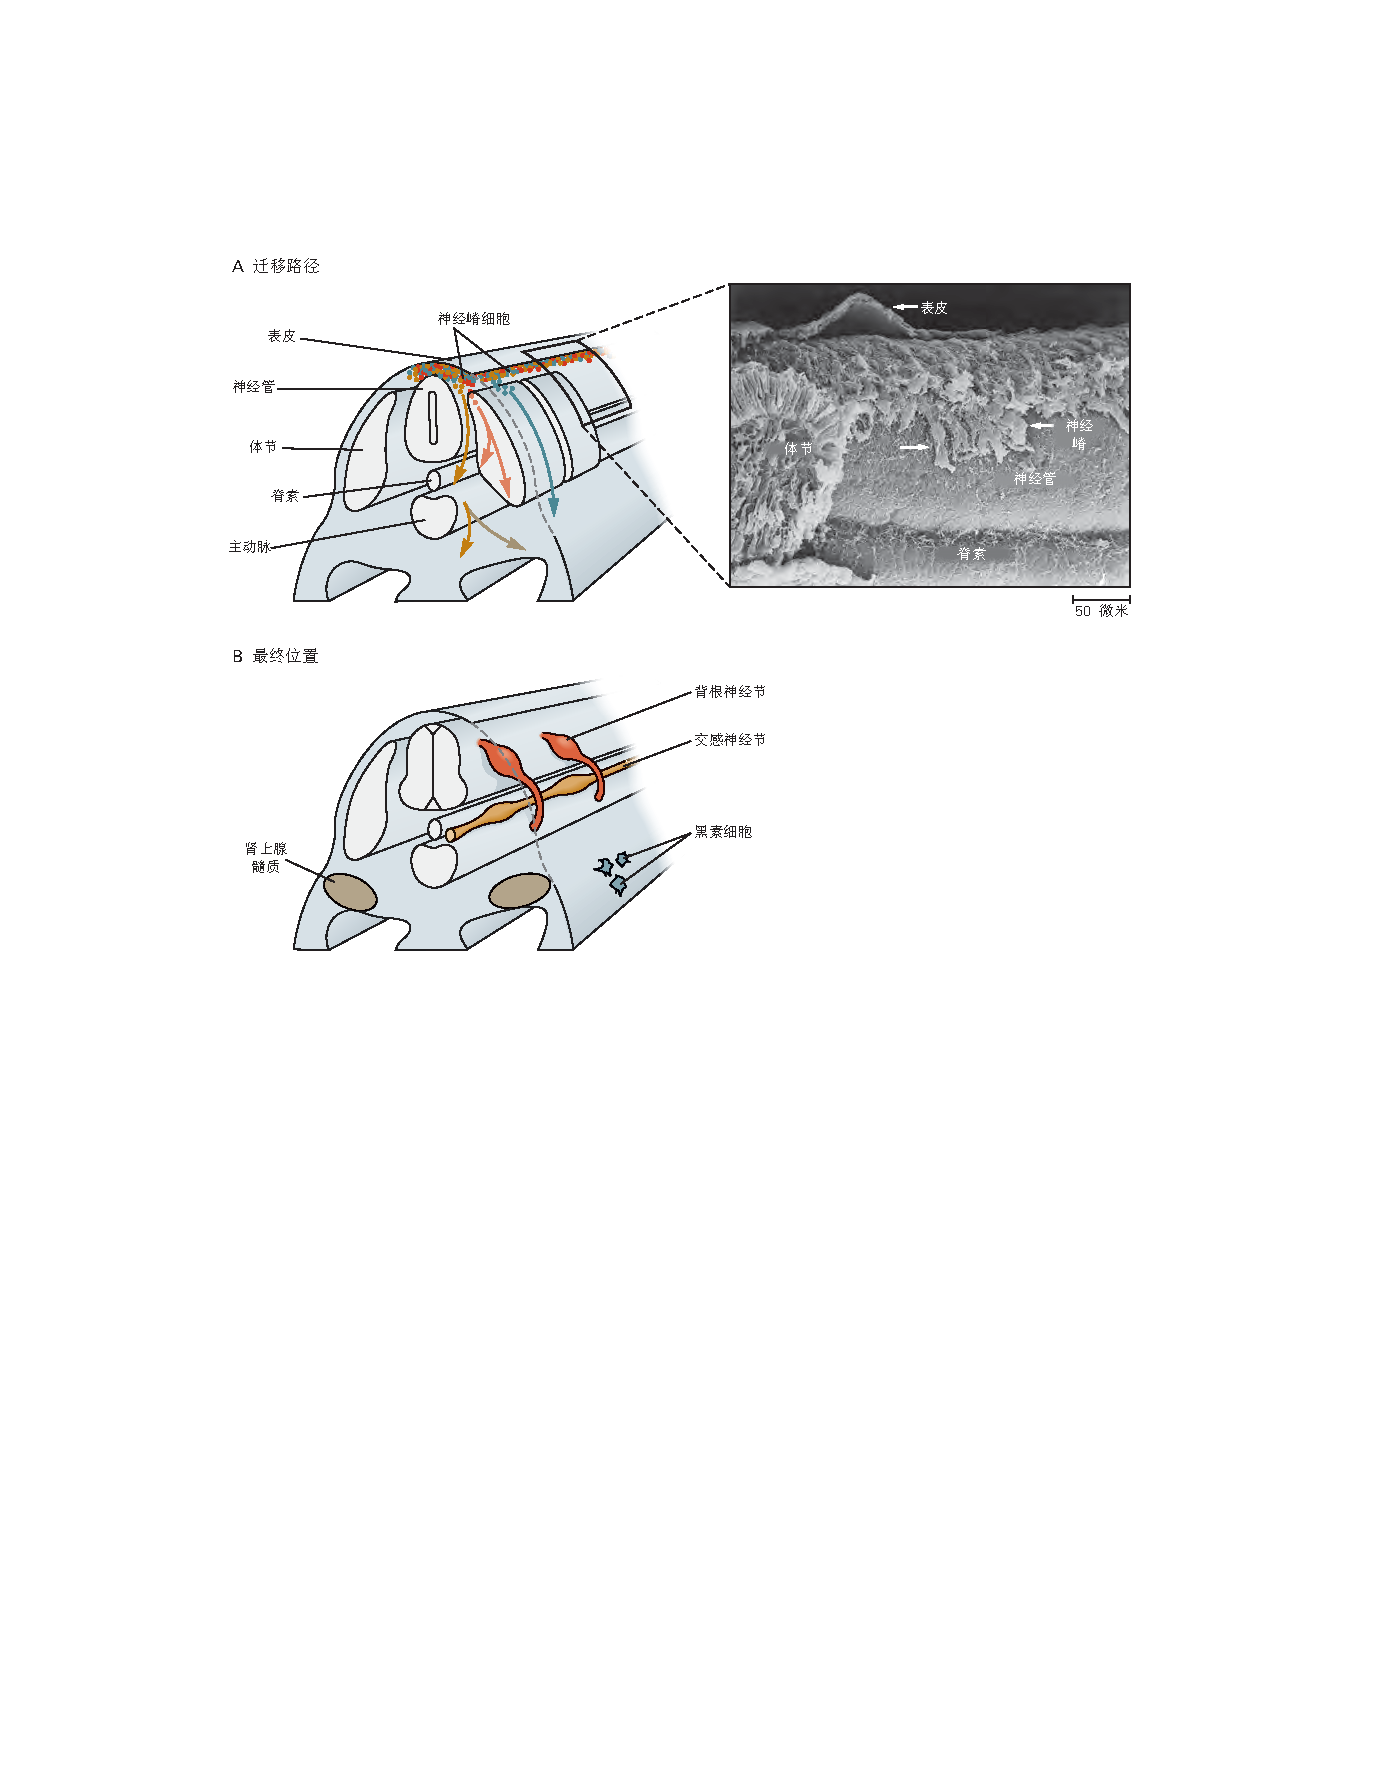
\includegraphics[width=1.0\linewidth]{chap46/fig_46_9}
	\caption{周围神经系统中的神经嵴细胞迁移。
		\textbf{A.} 鸡胚躯干中部的横截面显示了神经嵴细胞的主要通路。
		一些细胞沿着表层通路迁移,就在外胚层下方,并分化为皮肤的色素细胞。
		其他人沿着更深的路径迁移,使它们穿过体节,在那里它们结合形成背根感觉神经节。
		还有一些在神经管和体节之间迁移,经过背主动脉。
		这些细胞分化成交感神经节和肾上腺髓质。
		扫描电子显微照片显示神经嵴细胞从鸡胚神经管的背面迁移。
		\textbf{B.} 神经嵴细胞到达它们完成分化的最终沉降位置。}
	\label{fig:46_9}
\end{figure}


神经嵴迁移由几个分泌因子家族促进和引导。
例如,\textit{骨形态发生蛋白}对早期阶段的神经嵴诱导至关重要(第~\ref{chap:chap45}~章),而对于后期的神经嵴迁移则需要。
神经上皮细胞暴露于\textit{骨形态发生蛋白}会触发分子变化,将上皮细胞转化为间充质状态,导致它们从神经管分层并迁移到外周。
\textit{骨形态发生蛋白}通过诱导转录因子的表达触发神经嵴细胞的变化,特别是锌指蛋白蜗牛、slug 和 twist,它们在促进上皮-间充质转化方面具有保守作用。
这些转录因子直接表达调节细胞骨架特性的蛋白质以及降解细胞外基质蛋白质的酶。
这些酶使神经嵴细胞能够分解围绕神经管上皮细胞的基底膜,使它们能够开始向外周迁移的旅程。


随着神经嵴细胞开始分层,它们的细胞粘附分子表达发生变化。
粘附蛋白(尤其是钙粘蛋白)表达的改变允许神经嵴细胞松开与神经管细胞的粘附接触并开始分层过程。
神经嵴细胞也开始表达整合素,即细胞外基质蛋白的受体,例如沿外周迁移路径发现的层粘连蛋白和胶原蛋白。


迁移的神经嵴细胞遇到的第一个结构是体节,即后来产生肌肉和软骨的上皮细胞。
神经嵴细胞穿过每个体节的前半部分,但避开后半部分(图~\ref{fig:46_9}A)。
迁移神经嵴细胞的延髓通道是由肝配蛋白 B 蛋白施加的,这些蛋白集中在每个体节的后半部分。
\textit{轴突导向因子}提供一种排斥信号,该信号与神经嵴细胞上的 EphB 类酪氨酸激酶受体相互作用,以防止其入侵。
保留在体节前巩膜切开器内的神经嵴细胞分化为背根神经节的感觉神经元;
那些在体节背部区域周围迁移的细胞接近皮肤并产生黑素细胞。


神经嵴分化成其各种衍生物取决于细胞在其旅程中收到的不同线索与沿头尾轴变化的内在倾向之间的复杂相互作用。
感觉神经元的发育在细胞从神经管移出时开始。
细胞暴露于来自背神经管和体节的信号,这些信号诱导神经发生素(\textit{碱性螺旋环螺旋}家族的一种转录因子)的表达,进而促进感觉命运。
随后的影响使神经元多样化为多种感觉类型,例如伤害感受神经元和本体感受神经元(图~\ref{fig:46_10})。
相反,那些遵循更内侧和腹侧迁移路径的神经嵴细胞暴露于从背主动脉分泌的\textit{骨形态发生蛋白}。
它们表达\textit{碱性螺旋环螺旋}因子 Mash1,这导致它们分化为交感神经元。


\begin{figure}[htbp]
	\centering
	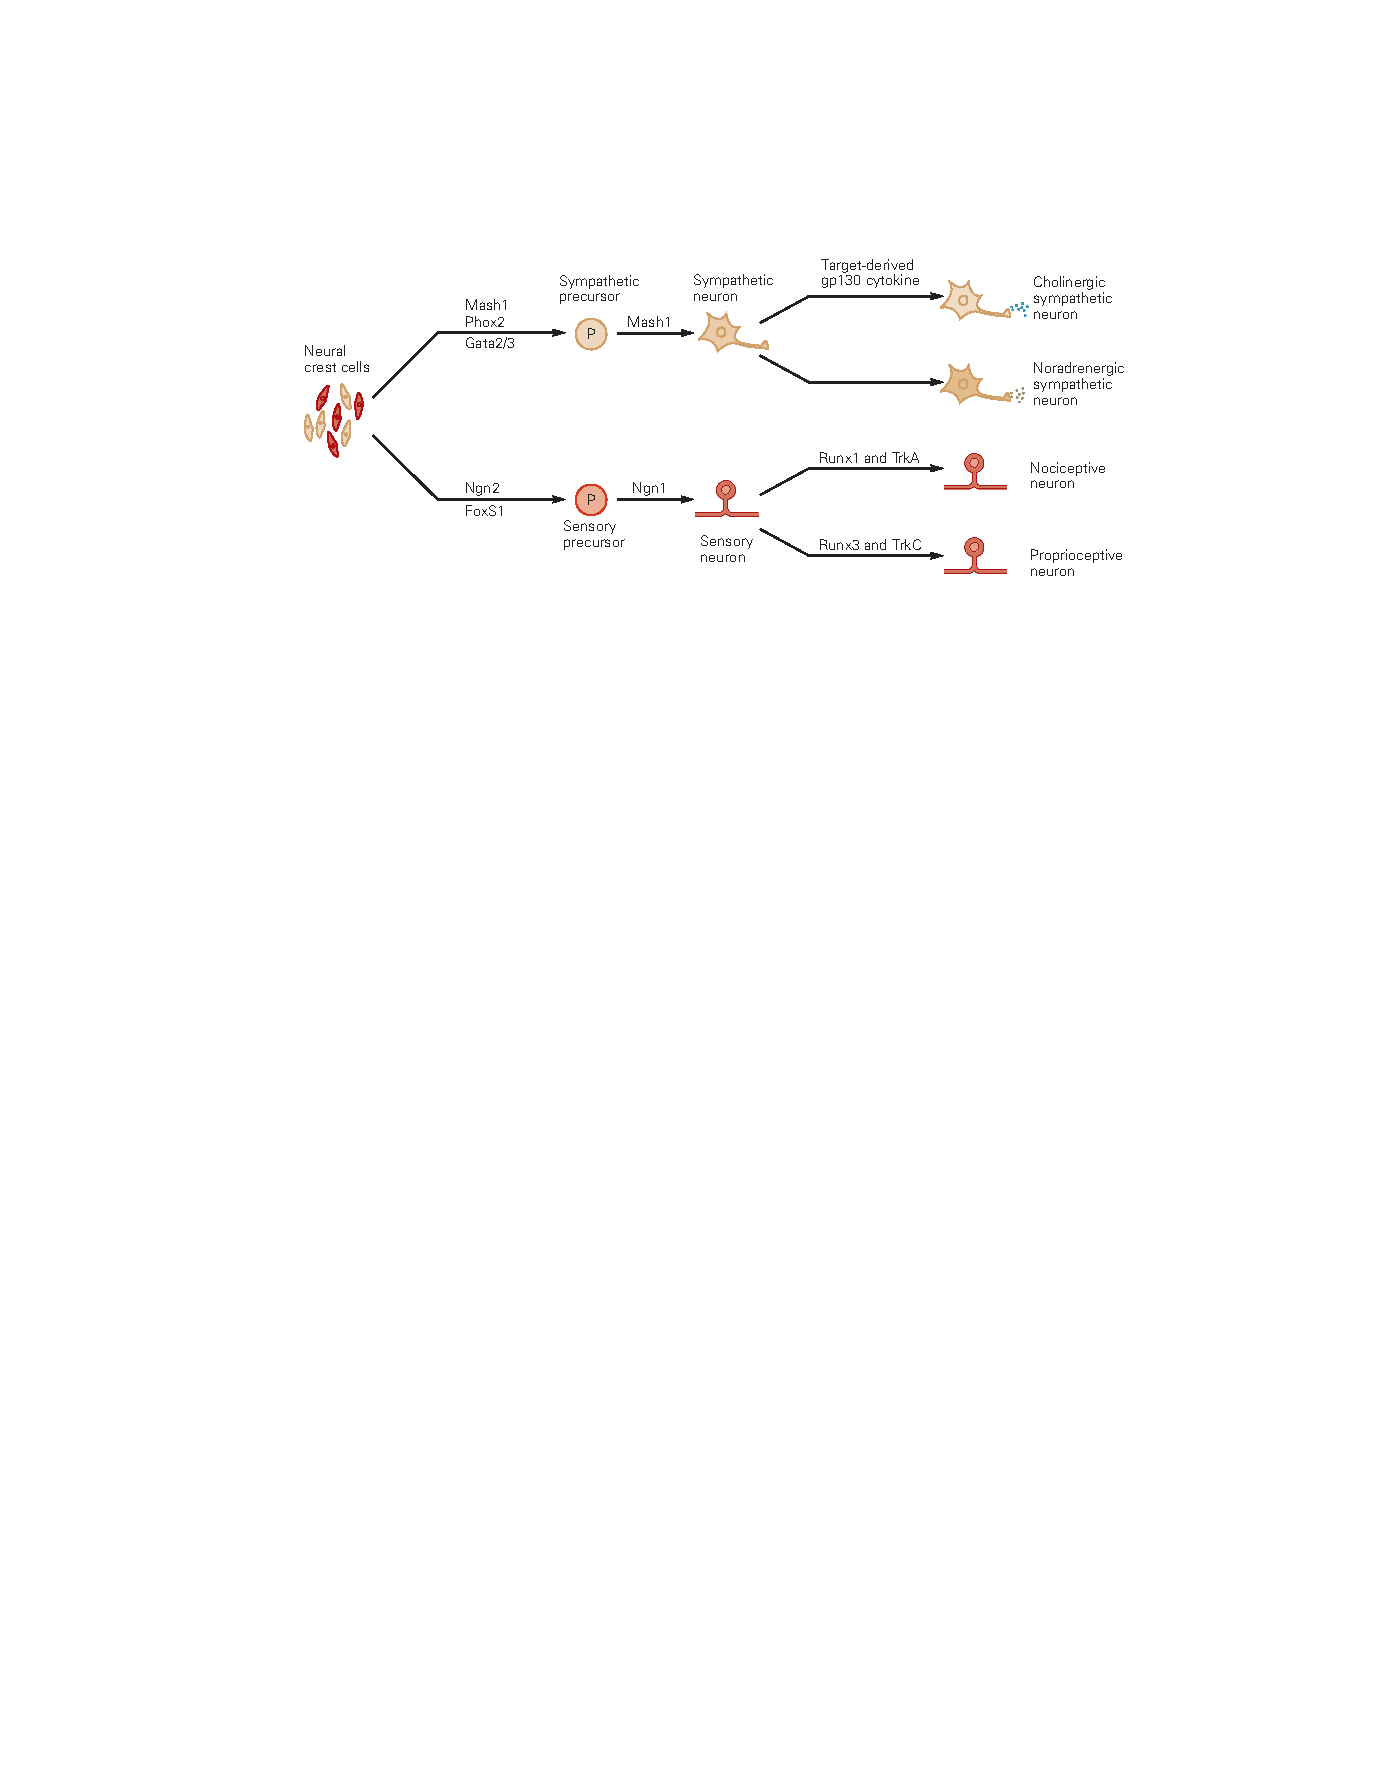
\includegraphics[width=1.0\linewidth]{chap46/fig_46_10}
	\caption{\textit{神经嵴细胞}分化为\textit{交感神经元}和\textit{感觉神经元}。
		躯干神经嵴细胞的神经元命运由转录因子表达控制。
		\textit{碱性螺旋环螺旋}蛋白 Mash1 的表达指导神经嵴细胞沿着交感神经元通路。
		交感神经元可以获得去甲肾上腺素能或胆碱能递质表型,这取决于它们支配的靶细胞和 gp130 细胞因子信号的水平(见图~\ref{fig:46_13})。
		两种\textit{碱性螺旋环螺旋}蛋白,neurogenin-1 和 -2,沿着感觉神经元通路引导神经嵴细胞。
		表达转录因子 Runx1 和酪氨酸激酶受体 \textit{酪氨酸激酶}A 的感觉神经元成为伤害感受器;
		那些表达 Runx3 和 \textit{酪氨酸激酶}C 的成为本体感受器。}
	\label{fig:46_10}
\end{figure}


\begin{figure}[htbp]
	\centering
	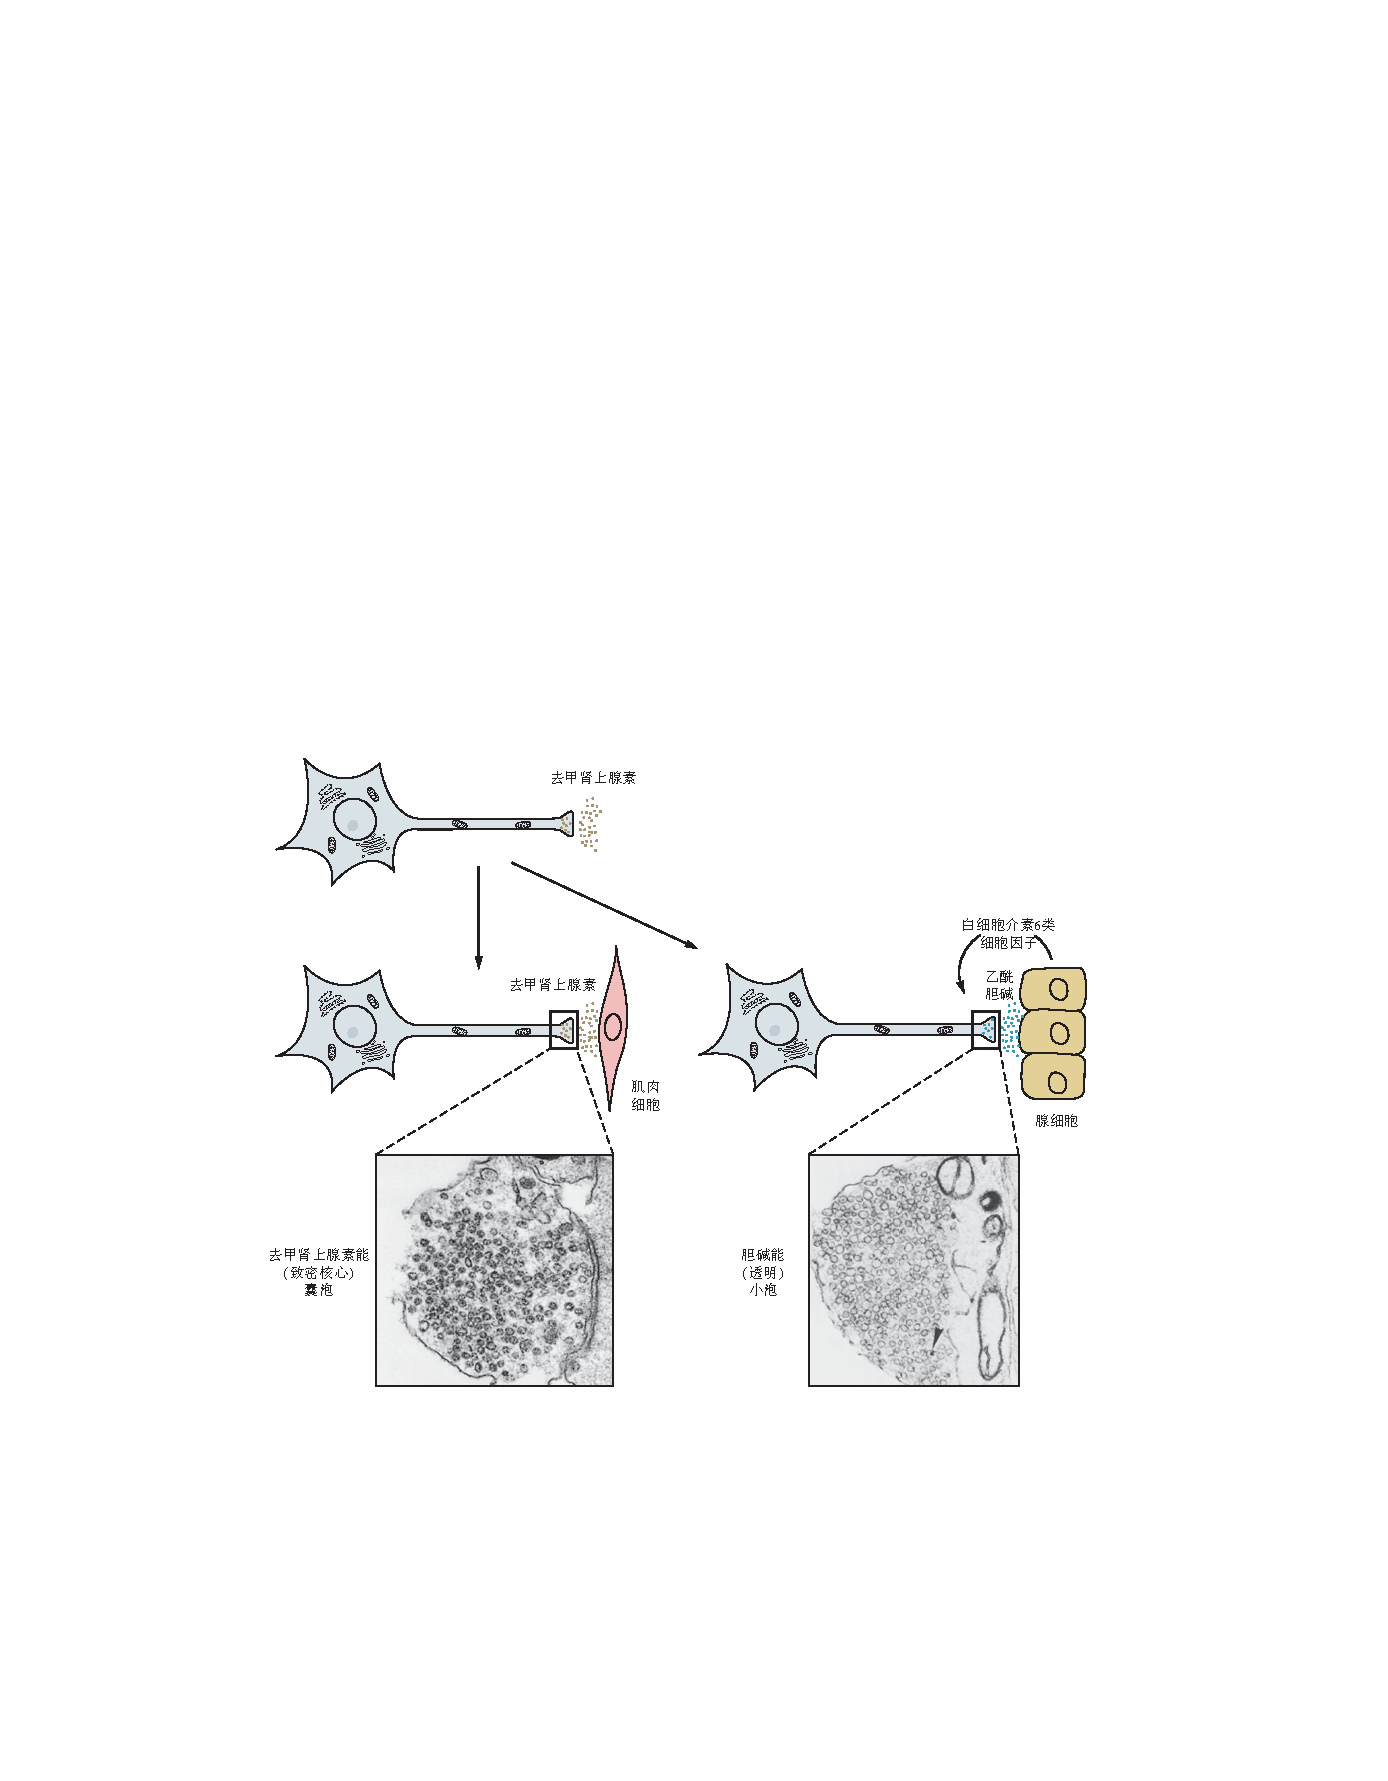
\includegraphics[width=1.0\linewidth]{chap46/fig_46_13}
	\caption{交感神经元的目标决定了神经递质表型。
		交感神经元最初被指定为具有去甲肾上腺素能递质表型。
		大多数交感神经元,包括那些支配心肌细胞的神经元,都保留了这种递质表型,它们的末端充满了储存去甲肾上腺素的致密核心囊泡。
		但是支配汗腺目标的交感神经元被诱导转换为胆碱能递质表型;
		它们的末端充满了储存\textit{乙酰胆碱}的透明小囊泡。
		汗腺细胞通过分泌白细胞介素细胞因子家族成员来指导开关。
		这个家族的几个成员,包括白血病抑制因子和睫状神经营养因子,是细胞培养中生长的交感神经元胆碱能表型的有效诱导剂。}
	\label{fig:46_13}
\end{figure}



\section{结构和分子创新是人类大脑皮层扩展的基础}

没有老鼠或猴子在读这本书。
这在很大程度上是因为人脑在质量和数量上都与我们最亲近的人的大脑不同。
然而,大多数哺乳动物神经发育研究都是在小鼠身上进行的,小鼠大脑中的神经元数量比人脑少大约 1 千倍,比研究最深入的非人灵长类动物恒河猴少 100 倍。
然而,最近,新的方法使阐明导致人类大脑特别是人类大脑皮层扩张的一些分子和结构特征成为可能。


经典的解剖学研究表明,灵长类动物的皮层不仅比啮齿类动物的尺寸和厚度大得多,而且具有更多的离散区域和更多层(图~\ref{fig:46_11}A)。
此外,灵长类动物的神经元堆积密度高于小鼠,因此神经元数量的差异大于仅从大小上预期的差异。
灵长类动物扩张的一个主要贡献者是大量的神经元祖细胞。
许多这些祖细胞是第二种类型的放射状神经胶质细胞,称为外放射状神经胶质细胞,以将其与上述典型或内放射状神经胶质细胞区分开来。
外放射状神经胶质细胞与内放射状神经胶质细胞不同,它与心室表面缺乏接触,并表现出与内放射状神经胶质细胞的分子差异。
然而,它们能够产生神经元并充当迁徙指南。
它们在灵长类动物,尤其是人类中数量的大量增加,部分解释了人类大脑皮层中神经元数量的增加。


\begin{figure}[htbp]
	\centering
	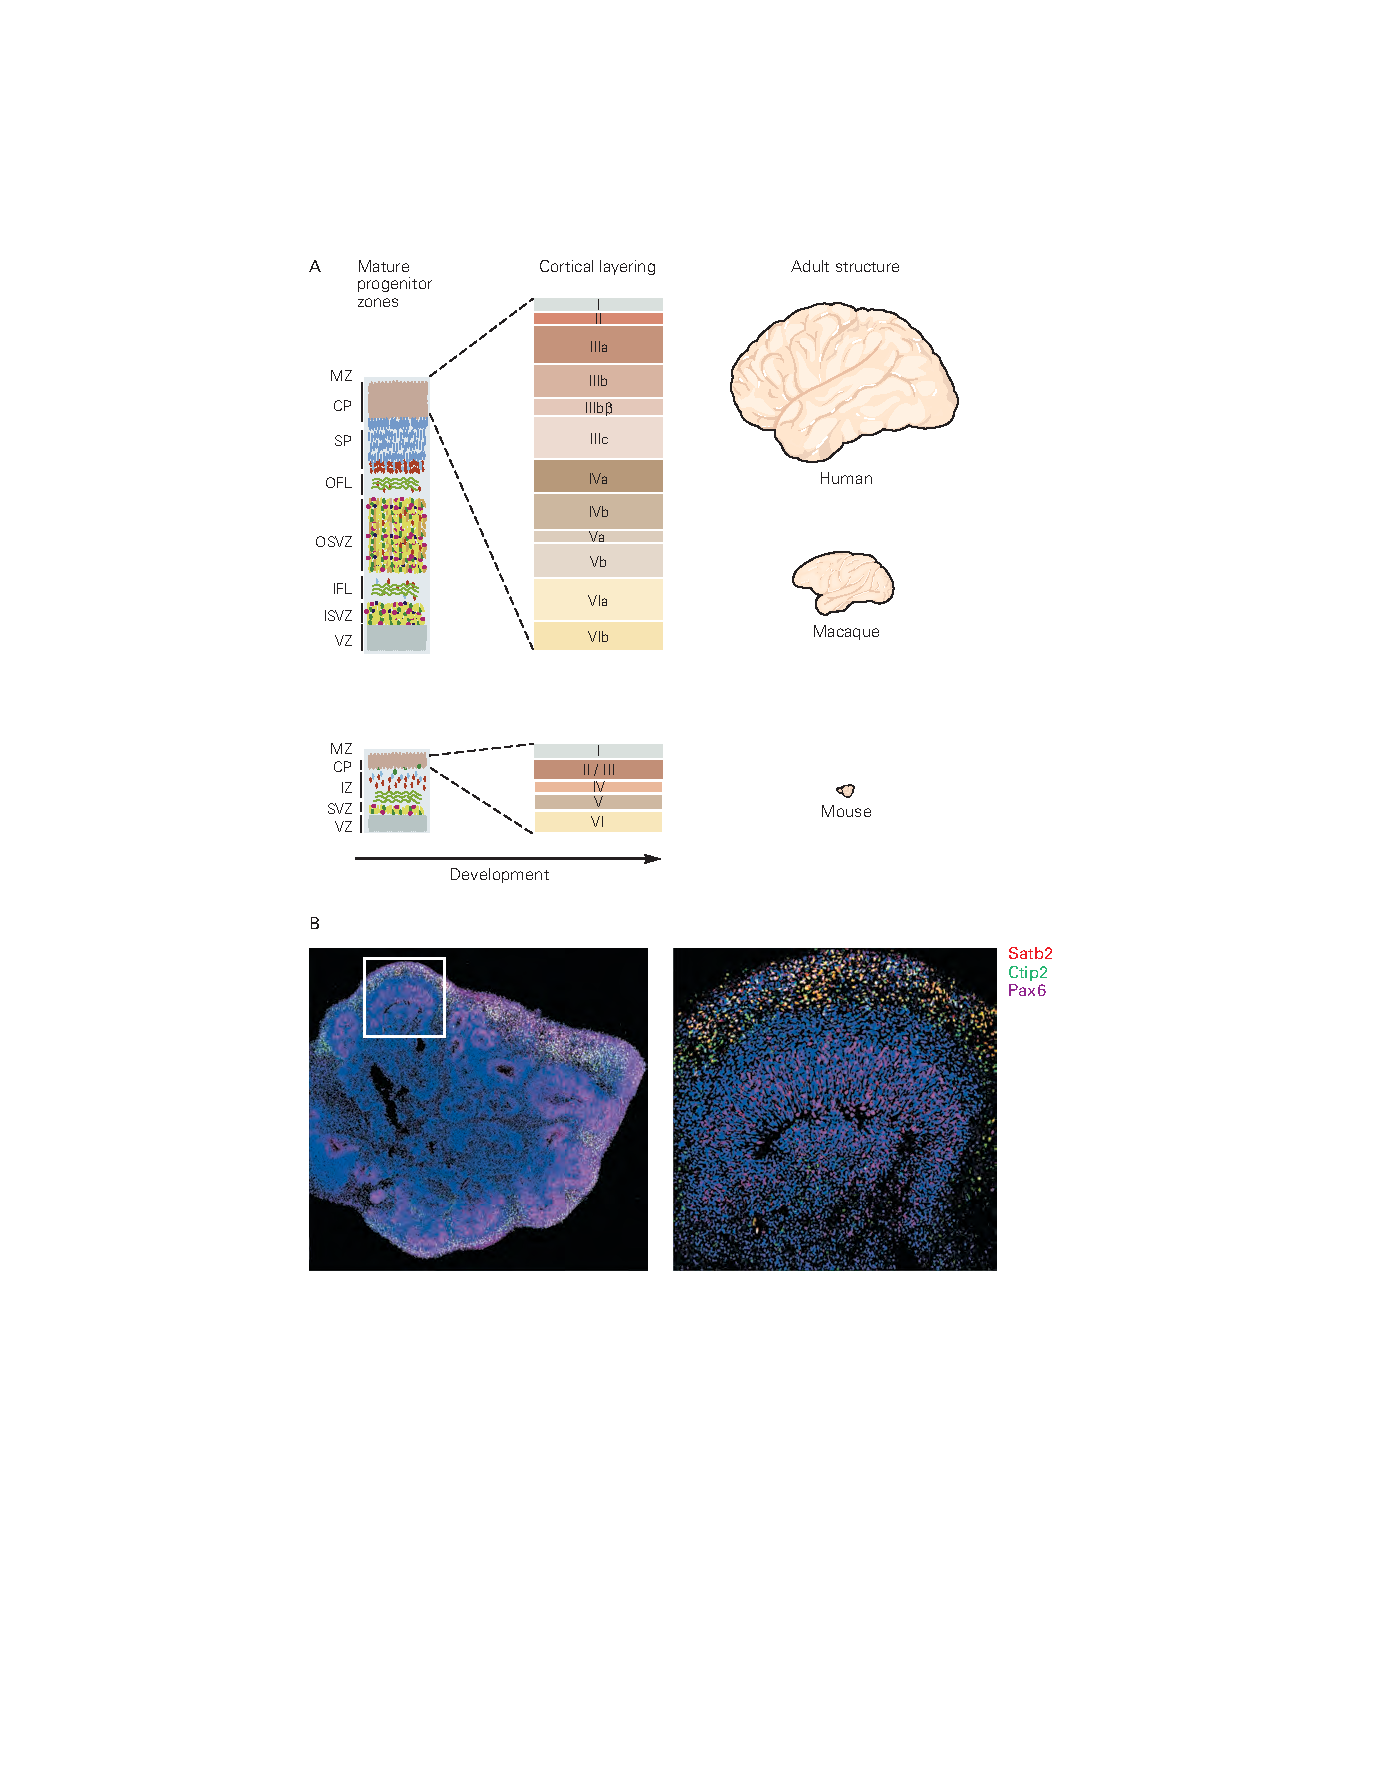
\includegraphics[width=1.0\linewidth]{chap46/fig_46_11}
	\caption{增殖区的扩大有助于人类和其他灵长类动物的皮层特化。
		\textbf{A.} 啮齿类动物和人类的神经上皮细胞大小最初都很小,但由于自我更新率的提高和人类祖细胞数量的增加,它们的相对大小随着发育的进行而显著不同。
		与小鼠相比,灵长类脑室下区大大扩大并细分为内部和外部区域,其中包含大量放射状神经胶质细胞,这两个区域都产生神经元。
		在小鼠中,几乎所有的放射状神经胶质细胞都属于内部类型\cite{giandomenico2017probing}。
		\textbf{B.} 由人类诱导的多能干细胞产生的类器官切片。
		在右侧的显微照片中,白线之间的区域被放大了。
		该部分用转录因子(Satb2、Ctip2 和 Pax6)的抗体染色,这些转录因子在人类皮层的特定层中选择性表达,表明类器官中形成了分层的皮层结构。}
	\label{fig:46_11}
\end{figure}


如何通过实验分析人类特有的发育特征?
新的分子分析方法使得将人类与我们近亲的蛋白质、转录物和基因进行比较成为可能,从而发现了有趣的专业化。
然而,从这些发现中得出的假设很难检验:
我们在这些章节中描述的大多数发育研究不能在人类身上进行,甚至非人类灵长类动物也是难以进行发育分析的对象。
一个可能的解决方案是最近设计的“类器官”培养系统。


来自成人皮肤的细胞可以通过我们将在第~\ref{chap:chap50}~章中讨论的方法重新编程成为称为\textit{诱导性多功能干细胞}的多能祖细胞。
当在小心控制的条件下进行培养并允许在三个维度上扩展时(与传统的二维文化截然不同),它们增殖并自我组织成类似于发育中的前脑的结构,并表现出物种特异性特征(图~\ref{fig:46_11}B)。
最值得注意的是,来自人类细胞的类器官包含一个双层的、大的脑室下区和许多外放射状神经胶质细胞,而来自小鼠细胞的类器官包含一个较小的脑室下区,主要包含常规或内放射状神经胶质细胞。
这些类器官可用于阐明人类皮层发育的至少某些早期方面的发育。


其他应用比比皆是。
一种是从患有脑部疾病的患者身上获取\textit{诱导性多功能干细胞}。
来自此类患者的类器官具有可能导致皮层畸形的特征,例如无脑畸形(见图~\ref{fig:46_5})。
希望这些类器官可用于阐明疾病机制并最终测试疗法。
第二个应用是比较源自黑猩猩和人类\textit{诱导性多功能干细胞}的类器官。
这种比较提供了一种新颖的方法来研究将我们与我们最亲近的现存亲戚区分开来的最新进化创新。



\section{内在程序和外在因素决定神经元的神经递质表型}

神经元在迁移到其最终位置后继续发育,并且它们后期分化的任何方面都比化学神经递质的选择更重要。
大脑中的神经元使用两种主要的神经递质:氨基酸 l-谷氨酸是主要的兴奋性递质,而$\gamma$-氨基丁酸是主要的抑制性递质。
一些脊髓神经元使用另一种氨基酸甘氨酸作为它们的抑制性递质。
在周围神经系统中,感觉神经元使用谷氨酸,运动神经元使用乙酰胆碱,自主神经元使用乙酰胆碱或去甲肾上腺素。
较少数量的神经元使用其他递质,例如血清素和多巴胺。
神经递质的选择决定了神经元可以与哪些突触后细胞交谈以及它可以说什么。



\subsection{神经递质的选择是神经元分化转录程序的核心组成部分}

不同的分子程序用于在不同的大脑区域和神经元类别中建立神经递质表型。
我们将通过关注大脑皮层和小脑中的神经元来说明分配氨基酸神经递质表型的一般策略。


大脑皮层包含在皮层板内产生的谷氨酸能锥体神经元,它们的分化依赖于\textit{碱性螺旋环螺旋}因子 neurogenin-1 和 neurogenin-2。
相反,正如本章前面所讨论的(参见图~\ref{fig:46_8}),大多数\textit{$\gamma$-氨基丁酸}能抑制性中间神经元从神经节隆起迁移到皮层;
它们的抑制性递质特性由\textit{碱性螺旋环螺旋}蛋白 Mash1(图~\ref{fig:46_12}A)以及 Dlx1 和 Dlx2 蛋白指定。


\begin{figure}[htbp]
	\centering
	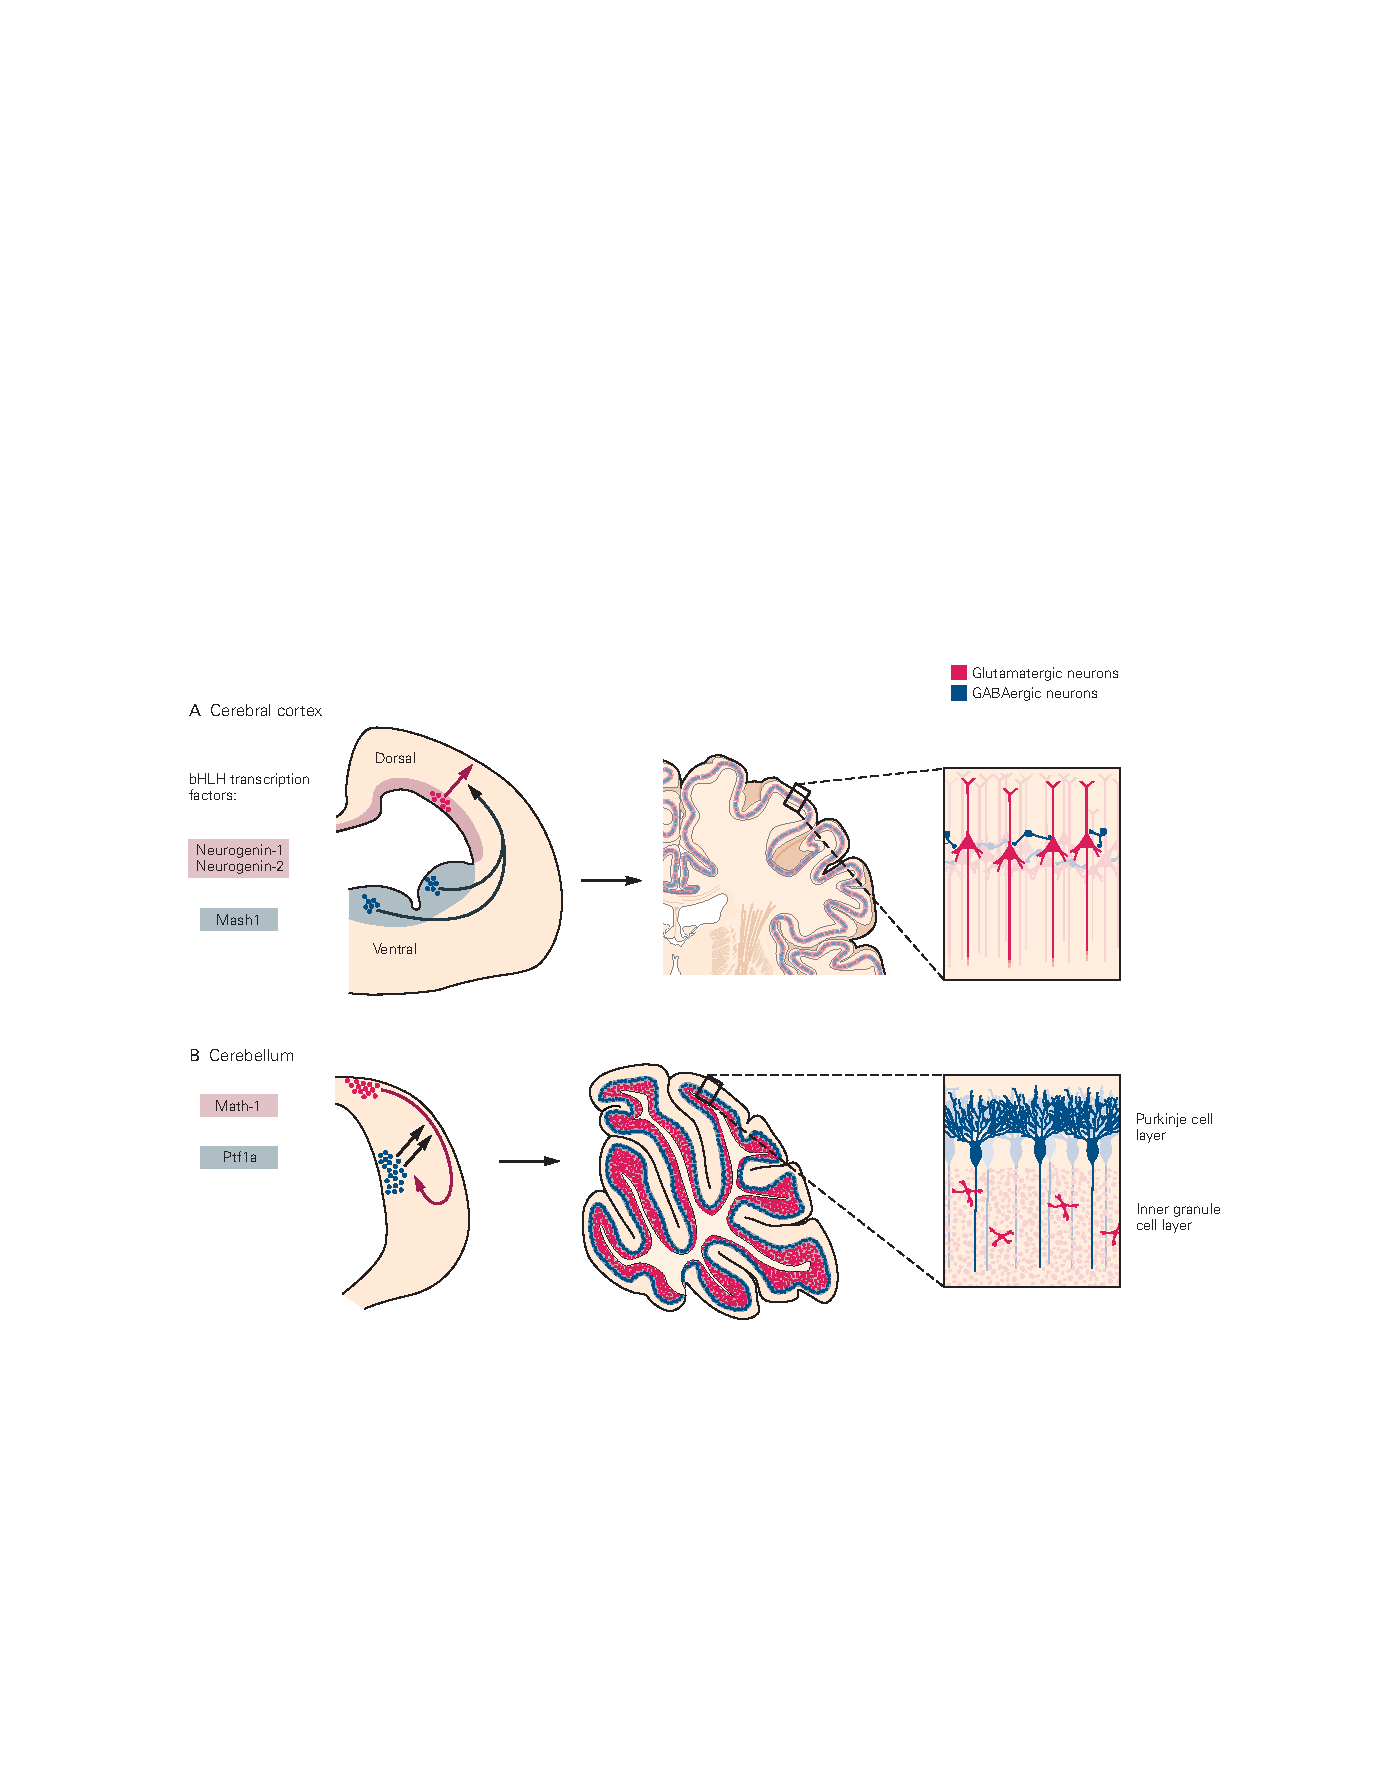
\includegraphics[width=1.0\linewidth]{chap46/fig_46_12}
	\caption{中枢神经元的神经递质表型由基本的螺旋-环-螺旋转录因子控制。
		\textbf{A.} 大脑皮层中的\textit{$\gamma$-氨基丁酸}能和谷氨酸能神经元在不同的增殖区产生,并由不同的\textit{碱性螺旋环螺旋}转录因子指定。
		谷氨酸能锥体神经元来源于皮层脑室区,它们的分化取决于神经生成素-1 和-2 的活性。
		腹侧端脑神经节隆突中\textit{$\gamma$-氨基丁酸}能中间神经元的分化取决于\textit{碱性螺旋环螺旋}蛋白 Mash1。
		这些神经元向背侧迁移,为大脑皮层提供大部分抑制性中间神经元。
		\textbf{B.} 发育中的小脑中的\textit{$\gamma$-氨基丁酸}能和谷氨酸能神经元也来自不同的增殖区,并由不同的\textit{碱性螺旋环螺旋}转录因子指定。
		谷氨酸能颗粒细胞从菱形唇迁移到小脑,沉降在内颗粒层,由\textit{碱性螺旋环螺旋}蛋白 Math-1 指定。
		\textit{$\gamma$-氨基丁酸能}浦肯野神经元从小脑深层增殖区迁移,定居在\textit{浦肯野细胞}层,并由\textit{碱性螺旋环螺旋}蛋白 Ptf1a 指定。}
	\label{fig:46_12}
\end{figure}


同样,小脑包含几种不同类别的抑制性神经元(浦肯野神经元、高尔基神经元、篮状神经元和星状神经元)和两大类兴奋性神经元(颗粒神经元和大小脑核神经元)。
这些抑制性和兴奋性神经元有不同的起源;
\textit{$\gamma$-氨基丁酸}能神经元来自脑室区,而谷氨酸能神经元从菱形唇迁移到小脑。
\textit{$\gamma$-氨基丁酸}能和谷氨酸能神经元的产生由两种不同的\textit{碱性螺旋环螺旋}转录因子控制,Ptf1a 用于抑制性神经元,Math-1 用于兴奋性神经元(图~\ref{fig:46_12}B)。
这些\textit{碱性螺旋环螺旋}因子由神经上皮细胞表达,但不由成熟神经元表达,这意味着分化为谷氨酸能和\textit{$\gamma$-氨基丁酸}能神经元是在神经元生成之前启动的。


转录程序还决定了周围神经系统中的递质表型。
例如,\textit{骨形态发生蛋白}通过诱导多种转录因子的表达来促进去甲肾上腺素能神经元分化,这些转录因子包括\textit{碱性螺旋环螺旋}蛋白 Mash1、同源域蛋白 Phox2 和锌指蛋白 Gata2。
相反,Runx 蛋白是感觉神经元谷氨酸能表型的决定因素(图~\ref{fig:46_10})。



\subsection{来自突触输入和目标的信号可以影响神经元的递质表型}

因为神经递质表型是核心神经元特性,所以长期以来人们认为神经递质特性在神经元分化的最早阶段是固定的。
这一观点受到研究的挑战,研究表明神经嵴细胞的迁移通路使细胞暴露于环境信号,这些信号在决定其递质表型方面具有关键作用。


大多数交感神经元使用去甲肾上腺素作为它们的主要递质。
然而,那些支配脚垫外分泌汗腺的神经元使用乙酰胆碱,甚至这些神经元在首次支配皮肤汗腺时也会表达去甲肾上腺素。
只有在它们的轴突接触到汗腺后,它们才会停止合成去甲肾上腺素并开始产生乙酰胆碱。


当新生大鼠脚垫上的汗腺被移植到通常由去甲肾上腺素能交感神经元支配的区域时,突触神经元获得胆碱能递质特性,表明汗腺细胞会分泌诱导交感神经元胆碱能特性的因子。


几种分泌因子触发交感神经元从去甲肾上腺素能表型转变为胆碱能表型。
汗腺分泌白细胞介素 6 样细胞因子的混合物,特别是心肌营养素 1、白血病抑制因子和睫状神经营养因子。
与递质合成和释放相关的神经元代谢的几个方面受这些因素控制。
神经元停止产生去甲肾上腺素能神经元特有的大致密核心颗粒,并开始产生胆碱能神经元典型的小电子半透明囊泡(图~\ref{fig:46_13})。


最近,越来越多的证据表明,中枢神经元的递质表型也会受到包括激素和电活动在内的信号的影响。
当胚胎两栖动物神经元的自发活动增加时,一些运动神经元可以重新指定合成和使用抑制性神经递质\textit{$\gamma$-氨基丁酸}代替或补充乙酰胆碱。
相反,当活动减少时,一些抑制性神经元转而使用兴奋性神经递质谷氨酸以及或代替\textit{$\gamma$-氨基丁酸}。
突触后伴侣通常会表达新的受体,这些受体与释放到它们上的递质相对应。
这些开关在没有对神经元进行整体重新指定的情况下发生,最好被视为旨在将系统的整体活动保持在狭窄范围内的稳态反应。


尽管中枢神经元中的这种递质开关在自然条件下可能很少发生,但活动依赖性神经递质可塑性可能是成人神经系统中更常见的现象。
例如,啮齿动物所在的光周期变化会导致负责维持昼夜节律的大脑区域使用多巴胺和生长抑素作为神经调节剂的神经元数量发生相互变化。
在这种情况和其他情况下,神经递质转换对动物的行为具有可衡量的影响,表明这一过程以及第~\ref{chap:chap49}~章中讨论的不太剧烈的突触变化被大脑用作对新环境的反应。



\section{神经元的存活受来自神经元靶标的神经营养信号的调节}

发育神经科学中更令人惊讶的发现之一是,胚胎神经系统中产生的大部分神经元最终在胚胎发育后期死亡。
同样令人惊讶的是,我们现在知道,细胞死亡的可能性在大多数动物细胞(包括神经元)中都是预先设定好的。
因此,关于生死的决定是神经元命运的各个方面。



\subsection{神经生长因子的发现证实了神经营养因子假说}

神经元的目标是神经元生存所必需的关键因素来源。
在对背根神经节的研究中发现了靶细胞在神经元存活中的关键作用。


在 1930 年代,\textit{塞缪尔$\cdot$戴特威勒}和\textit{维克多$\cdot$汉堡}发现胚胎中感觉神经元的数量通过将额外的肢芽移植到目标区域而增加,而如果移除肢体目标则减少。
当时,这些发现被认为反映了肢体对感觉神经元前体增殖和随后分化的影响。
然而,在 1940 年代,\textit{丽塔$\cdot$列维-蒙塔尔奇尼}做出了惊人的观察,即神经元的死亡不仅仅是病理学或实验操作的结果,而是发生在胚胎发育的正常程序中。
\textit{列维-蒙塔尔奇尼}和\textit{汉堡}继续证明,移除肢体会导致感觉神经元过度死亡,而不是它们的产生减少。


这些关于感觉神经元生死的早期发现很快扩展到中枢神经系统的神经元。
\textit{汉堡}发现,大约一半在脊髓中产生的运动神经元在胚胎发育过程中死亡。
此外,在类似于在感觉神经节上进行的实验中,\textit{汉堡}发现运动神经元死亡可以通过移除肢体而增加,并通过添加额外的肢体来减少(图~\ref{fig:46_14}A,B)。
这些发现表明,来自靶细胞的信号对于中枢神经系统和外周神经系统内神经元的存活至关重要。
在某些情况下,操纵突触活动会影响死亡的程度,可能是通过调节目标细胞产生的信号类型或数量来实现的(图~\ref{fig:46_14}C)。
我们现在知道,脊椎动物神经系统的大部分区域都会发生神经元过度生成,随后是神经元死亡阶段的现象。


\begin{figure}[htbp]
	\centering
	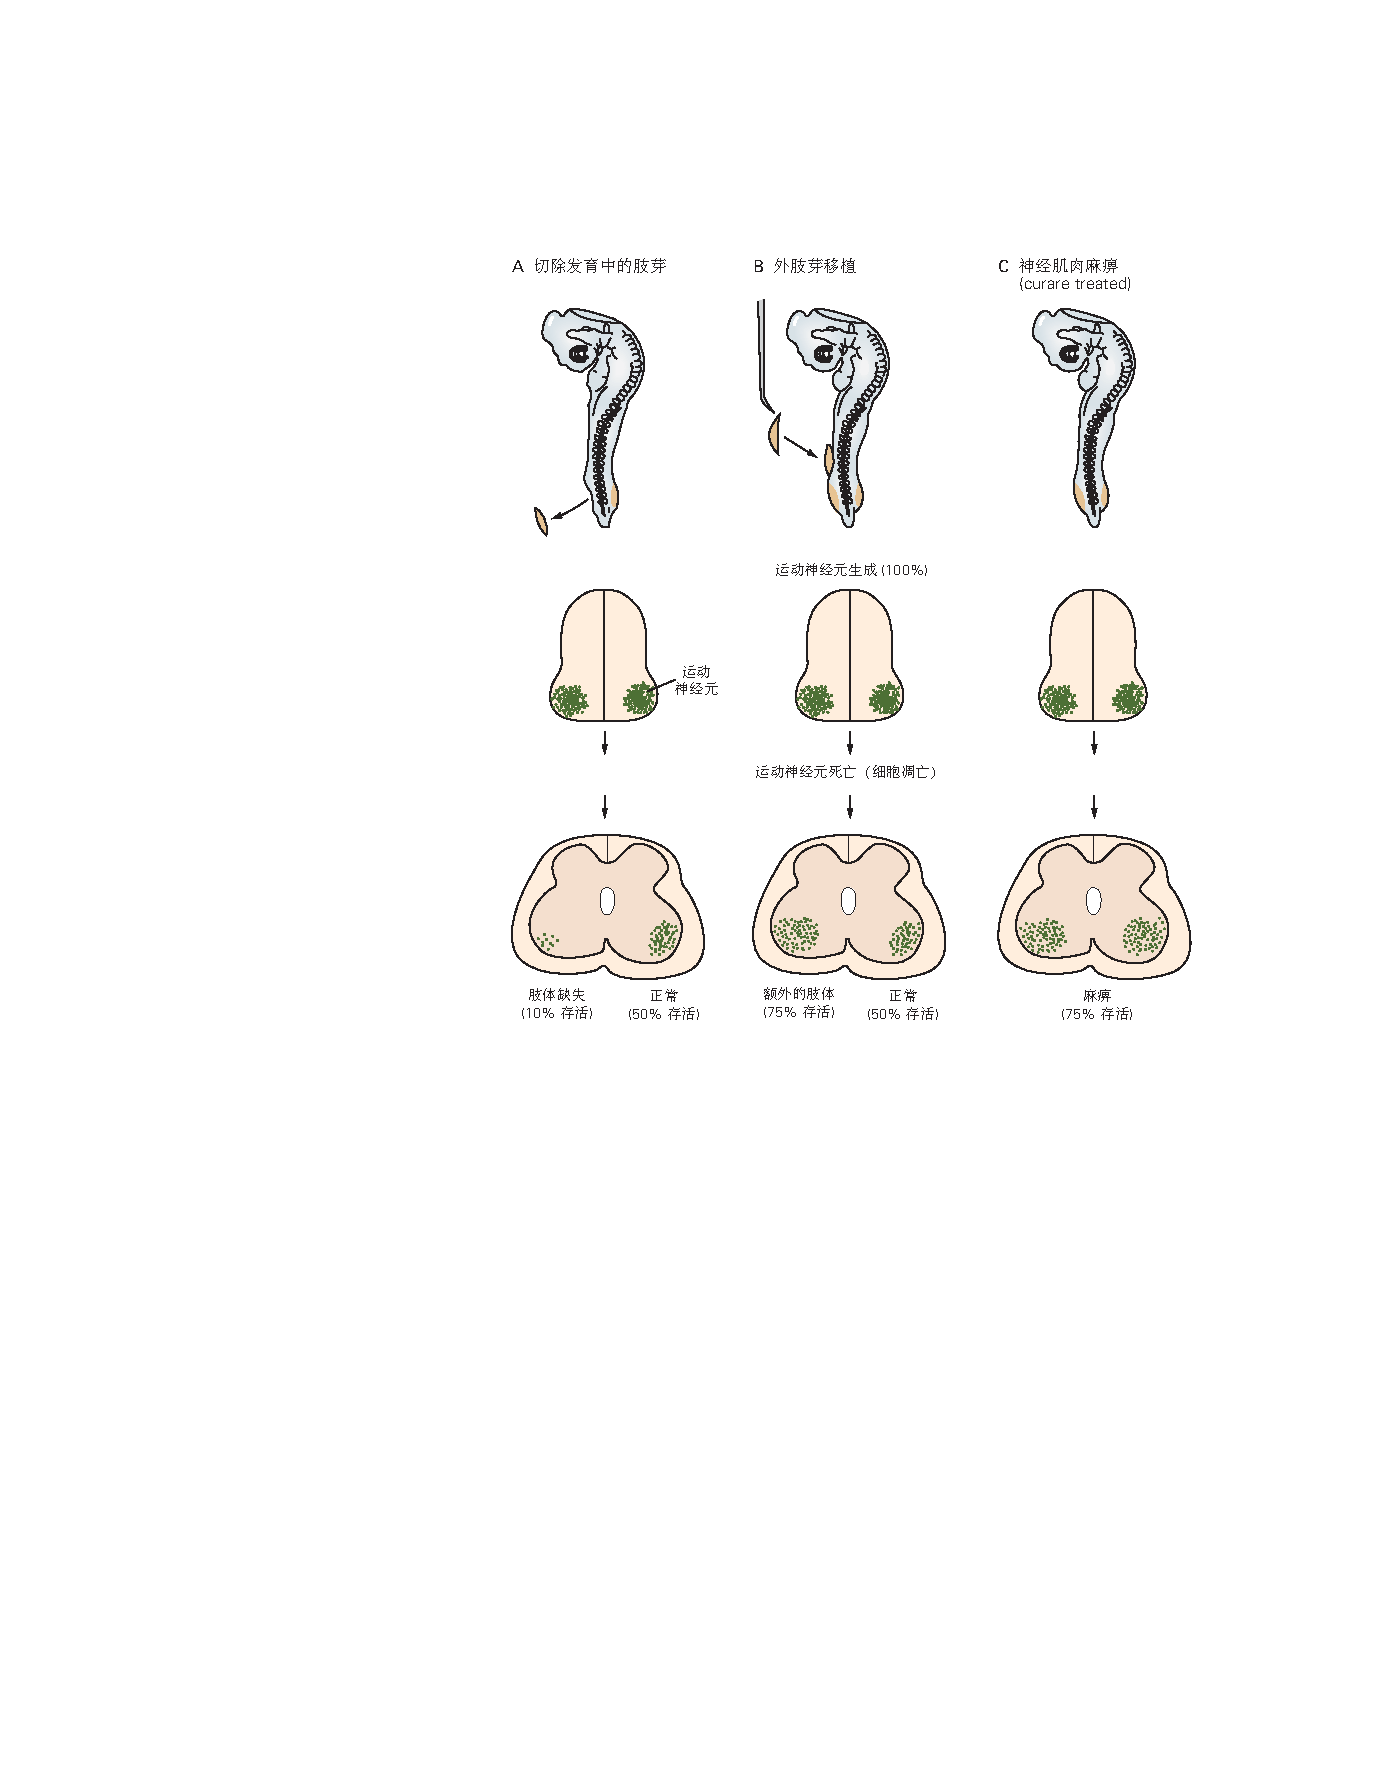
\includegraphics[width=0.85\linewidth]{chap46/fig_46_14}
	\caption{运动神经元的存活取决于其肌肉目标提供的信号。
		\textit{维克多$\cdot$汉堡}在对鸡胚进行的一系列经典实验中证明了肌肉目标在运动神经元存活中的作用\cite{purves1985principles}。
		\textbf{A.} 在运动神经到达后不久,从 2.5 天大的鸡胚中取出肢芽。
		1 周后的一段腰椎脊髓显示,在脊髓被剥夺的一侧几乎没有幸存的运动神经元。
		肢体完整的对侧运动神经元数量正常。
		\textbf{B.} 在正常的运动神经元死亡期之前,将一个额外的肢芽移植到宿主肢体附近。
		2 周后的一段腰椎脊髓显示多肢一侧的肢体运动神经元数量增加。
		\textbf{C.} 用箭毒毒素阻断神经肌肉活动,它可以阻断乙酰胆碱受体,挽救许多否则会死亡的运动神经元。
		箭毒可能通过增强非活动肌肉中营养因子的释放来发挥作用。}
	\label{fig:46_14}
\end{figure}


\textit{列维-蒙塔尔奇尼}和\textit{汉堡}的早期发现为神经营养因子假说奠定了基础。
该假设的核心是神经元靶点处或附近的细胞分泌少量必需营养素或营养因子,并且神经元存活需要神经末梢摄取该因子(图~\ref{fig:46_15})。
这一假设在 1970 年代得到了戏剧性的证实,当时 \textit{列维-蒙塔尔奇尼}和\textit{斯坦利$\cdot$科恩}纯化了我们现在称为\textit{神经生长因子}的蛋白质,并表明这种蛋白质是由靶细胞产生的,并支持体外感觉和交感神经元的存活。
此外,发现针对\textit{神经生长因子}的中和抗体会导致体内交感神经元和感觉神经元的严重损失。


\begin{figure}[htbp]
	\centering
	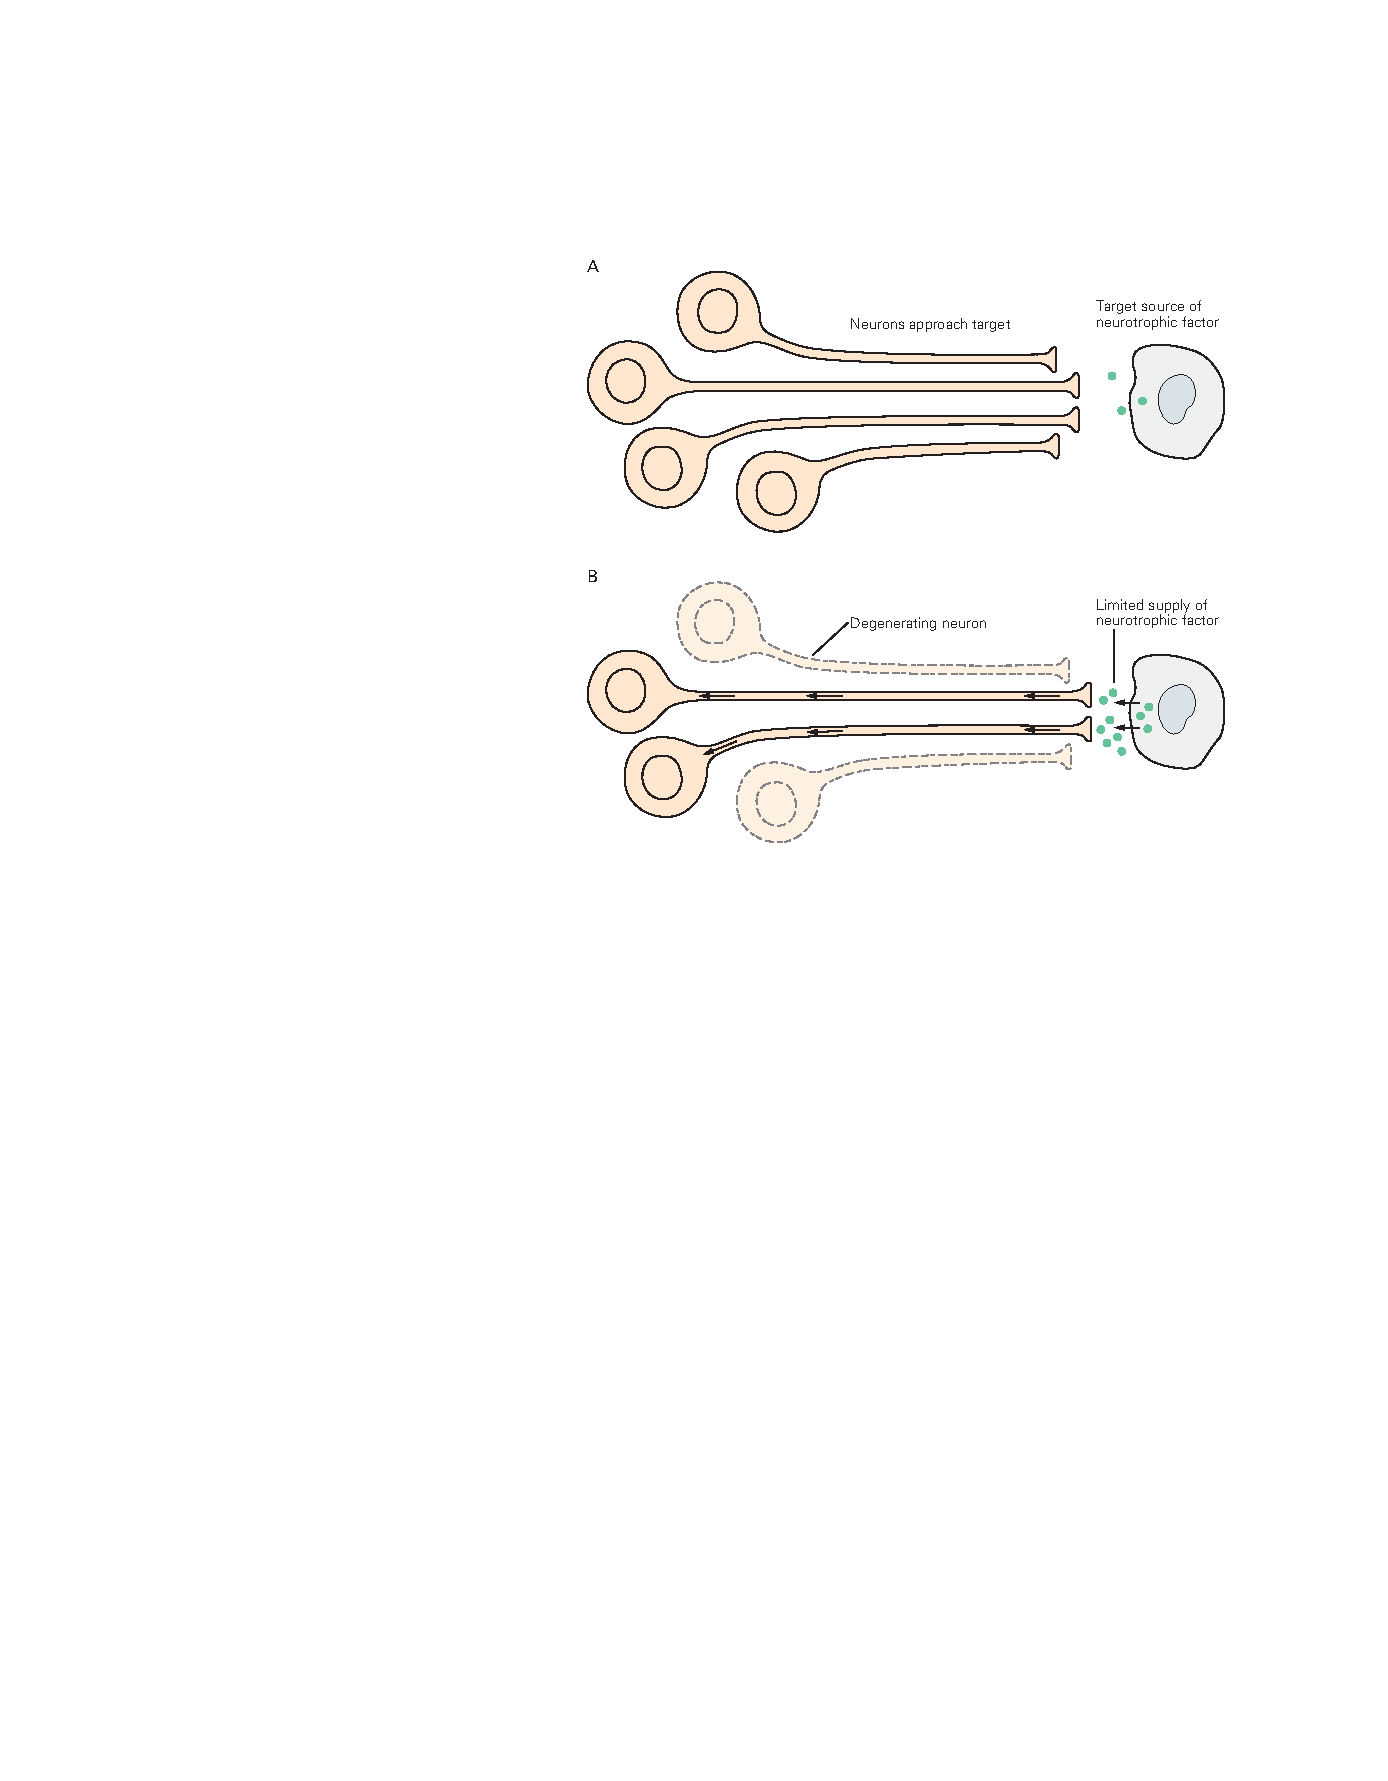
\includegraphics[width=0.84\linewidth]{chap46/fig_46_15}
	\caption{神经营养因子假说。
		\textbf{A.} 神经元将其轴突延伸至靶细胞,靶细胞分泌低水平的神经营养因子。
		(为简单起见,只显示了一个靶细胞。)
		神经营养因子与特定受体结合并被内化并运输到细胞体,在那里它促进神经元存活。
		\textbf{B.} 神经元无法获得足量的神经营养因子,通过称为细胞凋亡的细胞死亡程序死亡。}
	\label{fig:46_15}
\end{figure}



\subsection{神经营养因子是研究最透彻的神经营养因子}

\textit{神经生长因子}的发现促使人们开始寻找其他神经营养因子。
今天,我们知道有十几种促进神经元存活的分泌因子。
研究最多的与\textit{神经生长因子}相关,被称为神经营养蛋白家族。


有四种主要的神经营养因子:\textit{神经生长因子}本身、\textit{脑源性神经营养因子}以及\textit{神经营养因子}-3 和 \textit{神经营养因子}-4。
其他促进神经元存活的蛋白质类别包括转化生长因子 $ \beta $ 家族成员、白细胞介素 6 相关细胞因子、成纤维细胞生长因子,甚至我们之前遇到的某些诱导信号(\textit{骨形态发生蛋白}和刺猬蛋白)。
其他神经营养因子,特别是\textit{胶质细胞源性神经营养因子}家族的成员,负责不同类型的感觉和交感神经元的存活(图~\ref{fig:46_16})。


\begin{figure}[htbp]
	\centering
	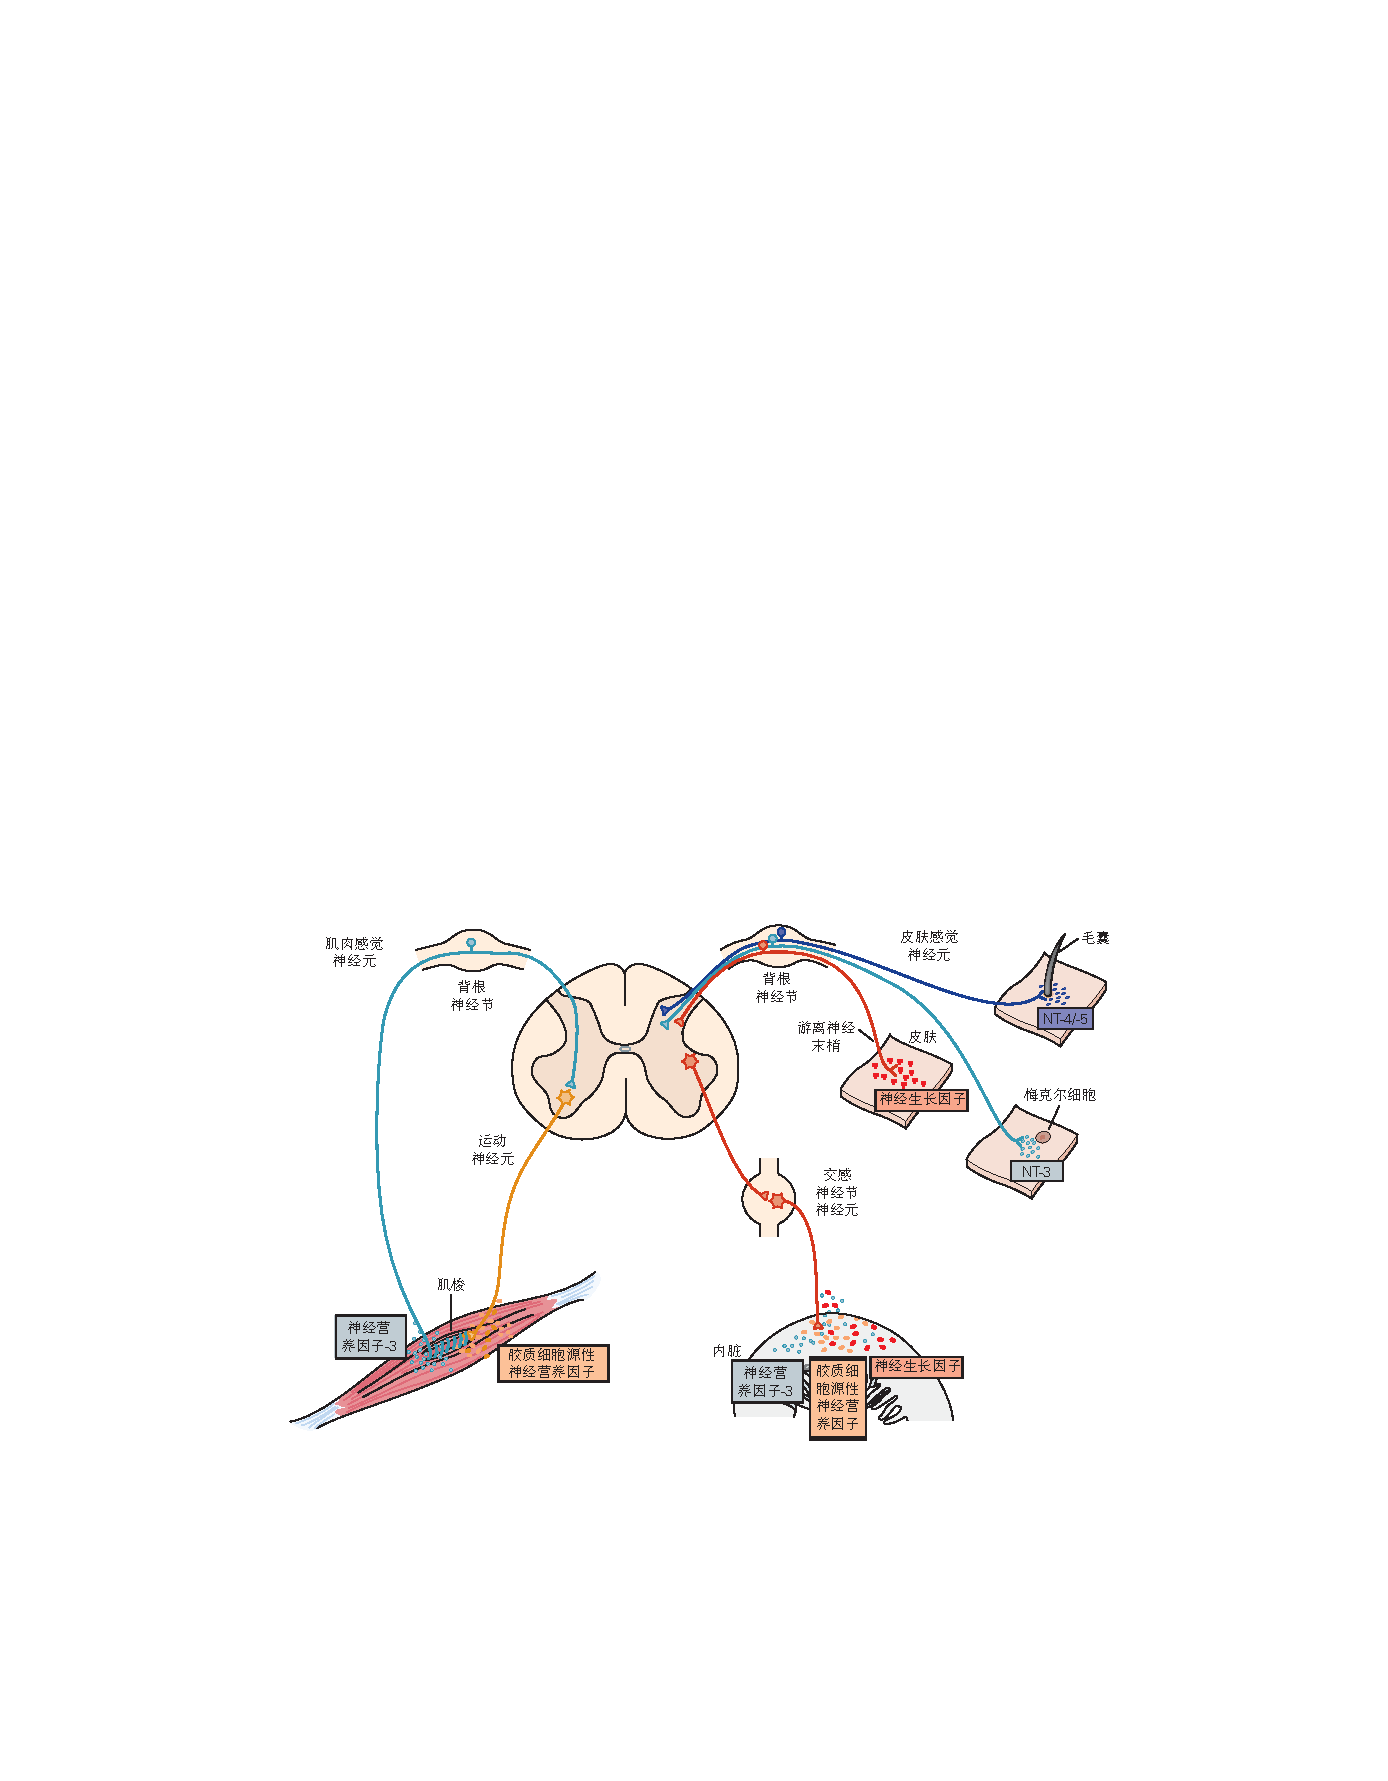
\includegraphics[width=1.0\linewidth]{chap46/fig_46_16}
	\caption{特定的神经营养因子促进不同群体的背根神经节神经元的存活。
		支配肌梭的本体感觉神经元依赖于\textit{神经营养因子}-3;
		支配皮肤的伤害性神经元依赖于\textit{神经生长因子}和神经营养素;
		支配\textit{梅克尔细胞}的机械感受神经元依赖于 \textit{神经营养因子}-3;
		那些支配毛囊的细胞依赖于\textit{神经营养因子}-4 和 \textit{神经营养因子}-5以及脑源性神经营养因子。
		运动神经元依赖于\textit{胶质细胞源性神经营养因子}和其他因素。
		交感神经元依赖于\textit{神经生长因子}、\textit{神经营养因子}-3 和 \textit{胶质细胞源性神经营养因子}\cite{reichardt1997neurotrophic}。}
	\label{fig:46_16}
\end{figure}


神经营养蛋白与两大类受体相互作用,即\textit{酪氨酸激酶}受体和 p75。
神经营养蛋白通过激活\textit{酪氨酸激酶}受体促进细胞存活。
\textit{酪氨酸激酶}家族包含三种跨膜酪氨酸激酶,名为\textit{酪氨酸激酶}A、\textit{酪氨酸激酶}B 和 \textit{酪氨酸激酶}C,每一种都以二聚体形式存在(图~\ref{fig:46_17})。


现在对神经营养蛋白与\textit{酪氨酸激酶}结合激活的细胞内信号通路了解很多。
与其他酪氨酸激酶受体一样,神经营养蛋白与\textit{酪氨酸激酶}受体的结合导致\textit{酪氨酸激酶}蛋白的二聚化。
二聚化导致激酶结构域激活环中特定酪氨酸残基的磷酸化。
这种磷酸化导致受体的构象变化和作为衔接蛋白对接位点的酪氨酸残基的磷酸化。
然后适配器触发第二信使的产生,这既促进神经元的存活又触发它们的成熟。
这些不同的生物反应涉及不同的细胞内信号传导途径:神经元分化主要通过\textit{有丝分裂原活化蛋白激酶}酶促途径,而存活主要通过磷脂酰肌醇 3 激酶途径(图~\ref{fig:46_18})。


\begin{figure}[htbp]
	\centering
	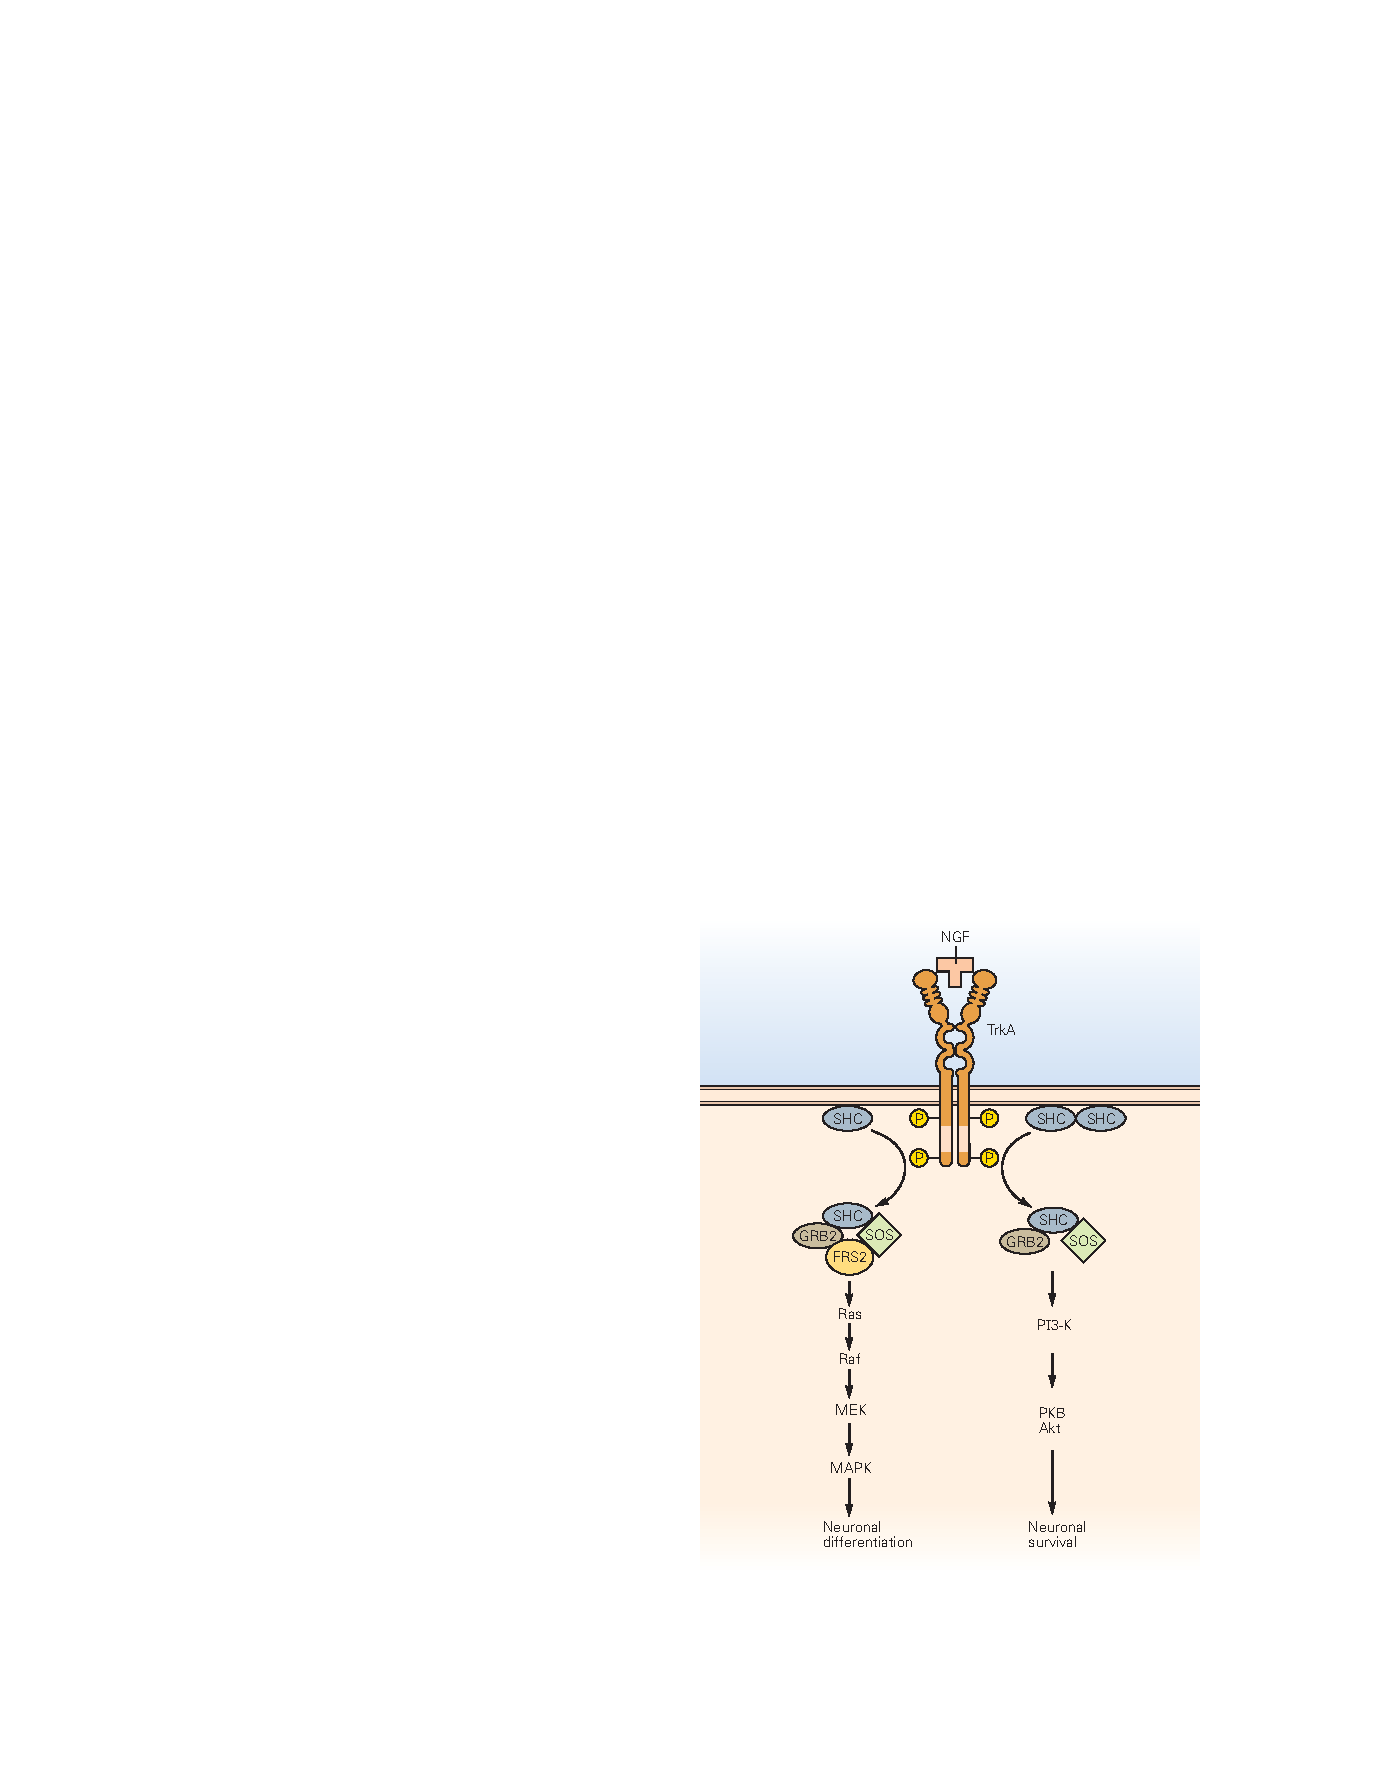
\includegraphics[width=0.67\linewidth]{chap46/fig_46_18}
	\caption{神经生长因子与\textit{酪氨酸激酶}A 受体的结合会激活替代的细胞内信号通路。
		\textit{神经生长因子}的结合诱导 \textit{酪氨酸激酶}A 受体的二聚化,从而触发其在许多不同残基处的磷酸化。
		\textit{酪氨酸激酶}A 的磷酸化导致衔接蛋白 SHC、GRB2 和 SOS 的募集。
		将 FRS2 额外募集到该复合体(左)会激活促进神经元分化的 Ras 激酶信号通路。
		在没有 FRS2(右)的情况下,该复合物激活促进神经元存活的\textit{磷酸肌醇3-激酶}通路。}
	\label{fig:46_18}
\end{figure}


与\textit{酪氨酸激酶}受体相互作用的特异性相反,所有神经营养蛋白都与受体 p75 结合(图~\ref{fig:46_17})。
在某些情况下,p75 与\textit{酪氨酸激酶}受体一起工作,调整\textit{酪氨酸激酶}对其神经营养蛋白配体的亲和力和特异性,从而促进神经元存活。
然而,p75 却过着双重生活。
它还可以结合未加工的神经营养蛋白前体,称为原神经营养蛋白,并且可以与其他称为分选蛋白的膜受体结合。
\textit{神经营养素}与 p75/sortilin 复合物的结合促进神经元死亡。
受体 p75 是\textit{肿瘤坏死因子}受体家族的成员,通过激活半胱天冬酶家族的蛋白酶来促进细胞死亡,我们将在下面讨论。


\begin{figure}[htbp]
	\centering
	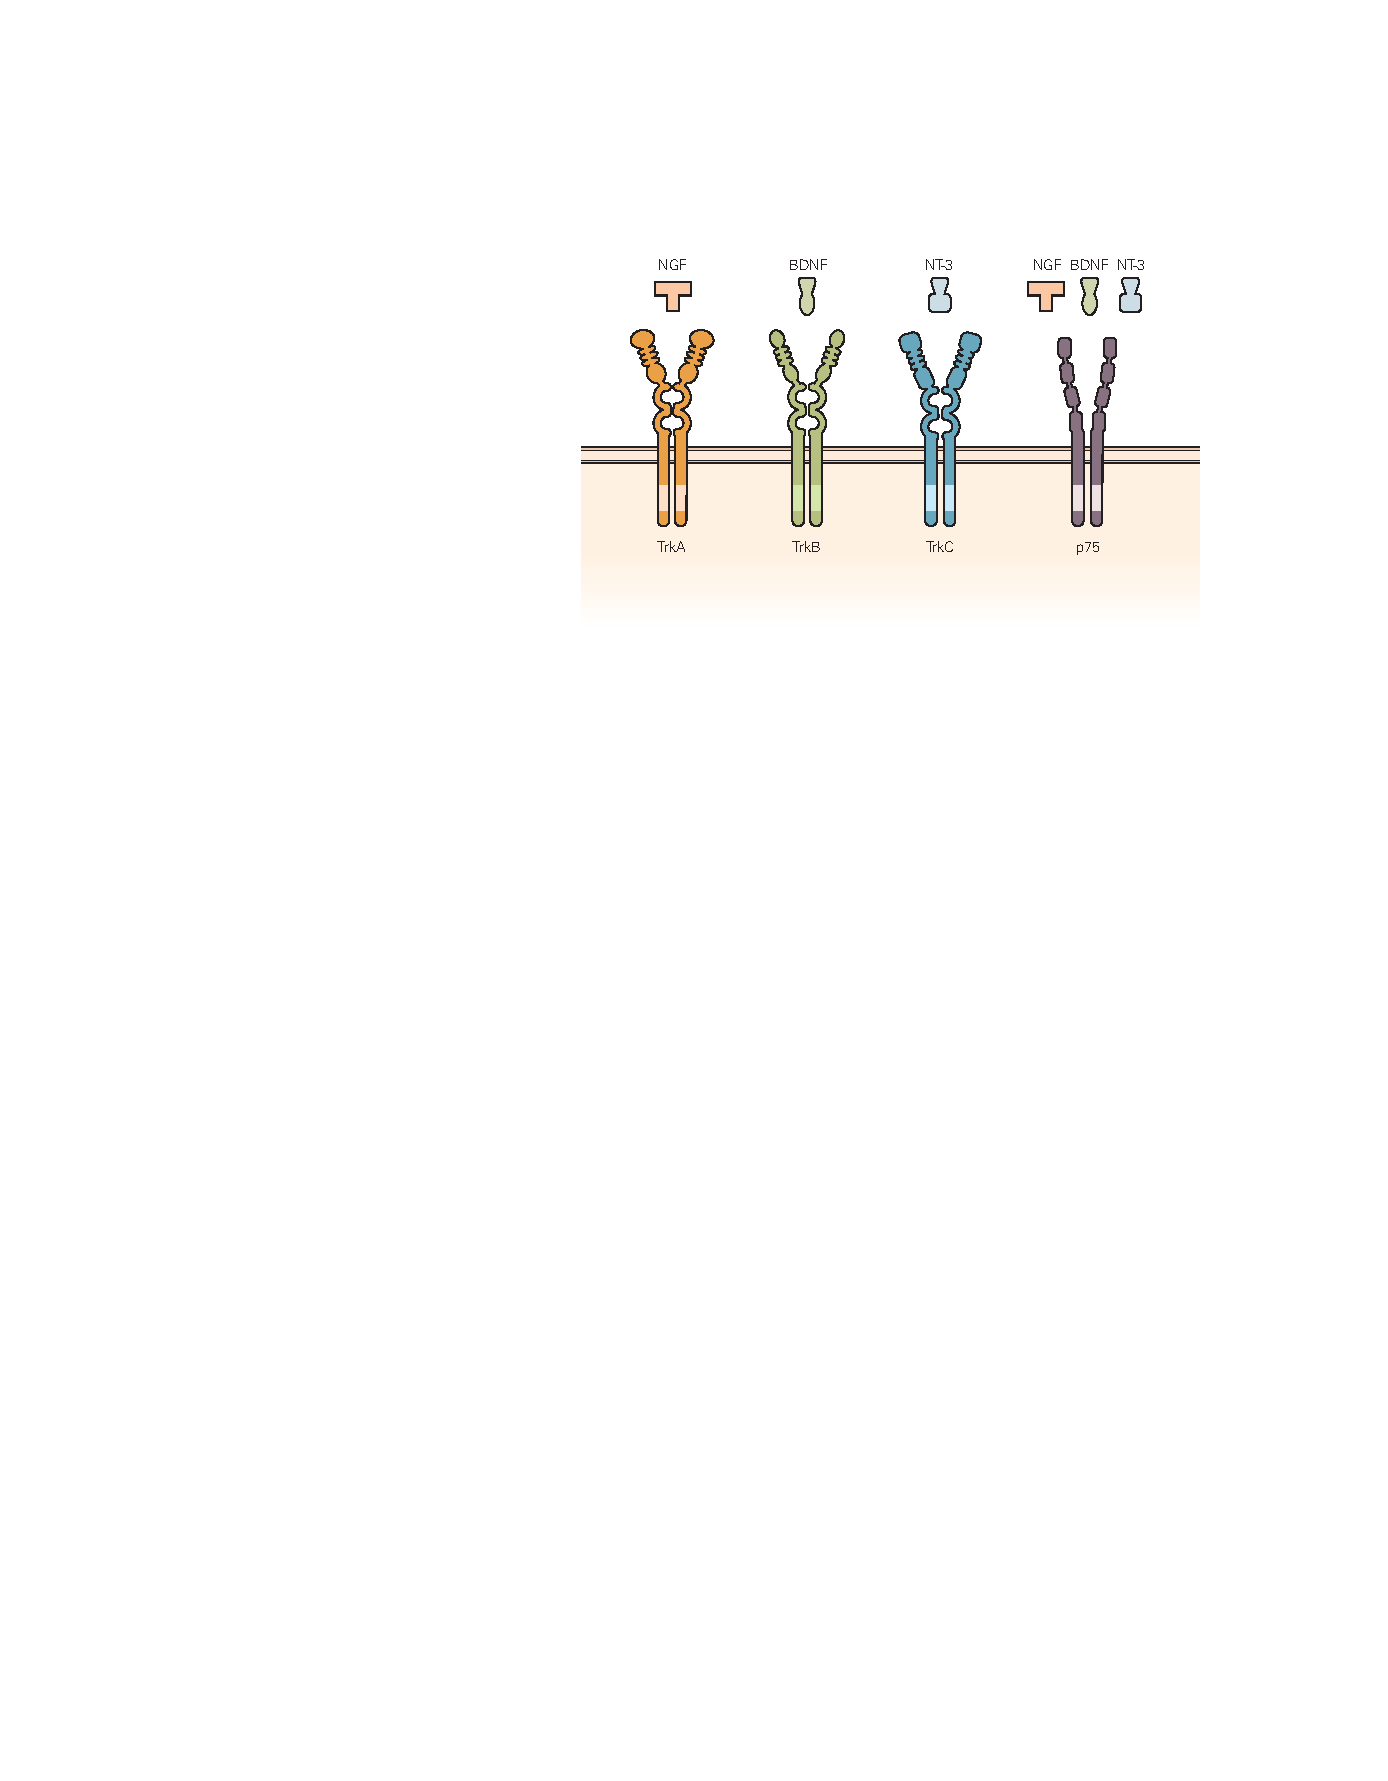
\includegraphics[width=0.81\linewidth]{chap46/fig_46_17}
	\caption{神经营养因子及其受体。
		三种主要神经营养蛋白中的每一种都与不同的跨膜\textit{酪氨酸激酶}相互作用。
		此外,所有三种神经营养蛋白都可以与低亲和力神经营养蛋白受体 p75 结合\cite{reichardt1997neurotrophic}。}
	\label{fig:46_17}
\end{figure}


神经营养蛋白信号通过一个涉及与\textit{酪氨酸激酶}受体结合的神经营养蛋白复合物内化的过程从轴突末端传递到神经元的细胞体。
这种复合物的逆行运输发生在一类称为信号内体的内吞小泡中。
这些囊泡的运输将激活的\textit{酪氨酸激酶}受体带入细胞区室,能够激活神经元存活、成熟和突触分化所必需的信号通路和转录程序。


对于中枢神经系统中的神经元,情况更为复杂。
例如,运动神经元的存活不依赖于单一的神经营养因子。
相反,不同类别的运动神经元需要由肌肉或外周神经胶质细胞表达的神经营养因子、\textit{胶质细胞源性神经营养因子}和白细胞介素 6 样蛋白。
这些神经元类别的存活取决于轴突对局部神经营养因子的暴露。



\subsection{神经营养因子抑制潜伏细胞死亡程序}

神经营养因子曾被认为通过以有益的方式刺激神经细胞的新陈代谢来促进神经细胞的存活,因此得名。
然而,现在很明显,神经营养因子抑制了身体所有细胞(包括神经元)中存在的潜在死亡程序。


这种生化途径可以被认为是一种自杀程序。
一旦它被激活,细胞就会因细胞凋亡而死亡:
它们聚集起来,形成气泡,浓缩染色质,并破碎细胞核。
凋亡性细胞死亡与坏死不同,坏死通常由急性外伤引起,涉及细胞膜的快速裂解而不激活细胞死亡程序。


剥夺神经营养因子通过释放活跃的生化程序杀死神经元的第一个线索来自评估抑制\textit{核糖核酸}和蛋白质合成后神经元存活的研究。
发现将交感神经元暴露于蛋白质合成抑制剂可防止由去除\textit{神经生长因子}引发的交感神经元死亡。
这些结果引发了这样的想法,即神经元有能力合成致命的蛋白质,而\textit{神经生长因子}会阻止它们的合成,从而抑制内源性细胞死亡程序。


对内源性细胞死亡程序的生化性质的重要见解来自线虫秀丽隐杆线虫的遗传研究。
在秀丽隐杆线虫的发育过程中,会产生精确数量的细胞,并死掉固定数量的这些细胞(胚胎与胚胎之间的数量相同)。
这些发现促使人们对阻断或增强细胞死亡的基因进行筛选,从而鉴定出\textit{细胞死亡}基因。
其中两个基因,\textit{细胞死亡}-3 和 \textit{细胞死亡}-4,是神经元死亡所必需的;
在它们不存在的情况下,每一个注定要死亡的细胞都会存活下来。

第三个基因 \textit{细胞死亡}-9 是生存所必需的,它通过拮抗 \textit{细胞死亡}-3 和 \textit{细胞死亡}-4 的活性发挥作用(图~\ref{fig:46_19})。
因此,在没有 \textit{细胞死亡}-9 的情况下,许多额外的细胞死亡,即使这些死亡仍然依赖于 \textit{细胞死亡}-3 和 \textit{细胞死亡}-4 活性。


\begin{figure}[htbp]
	\centering
	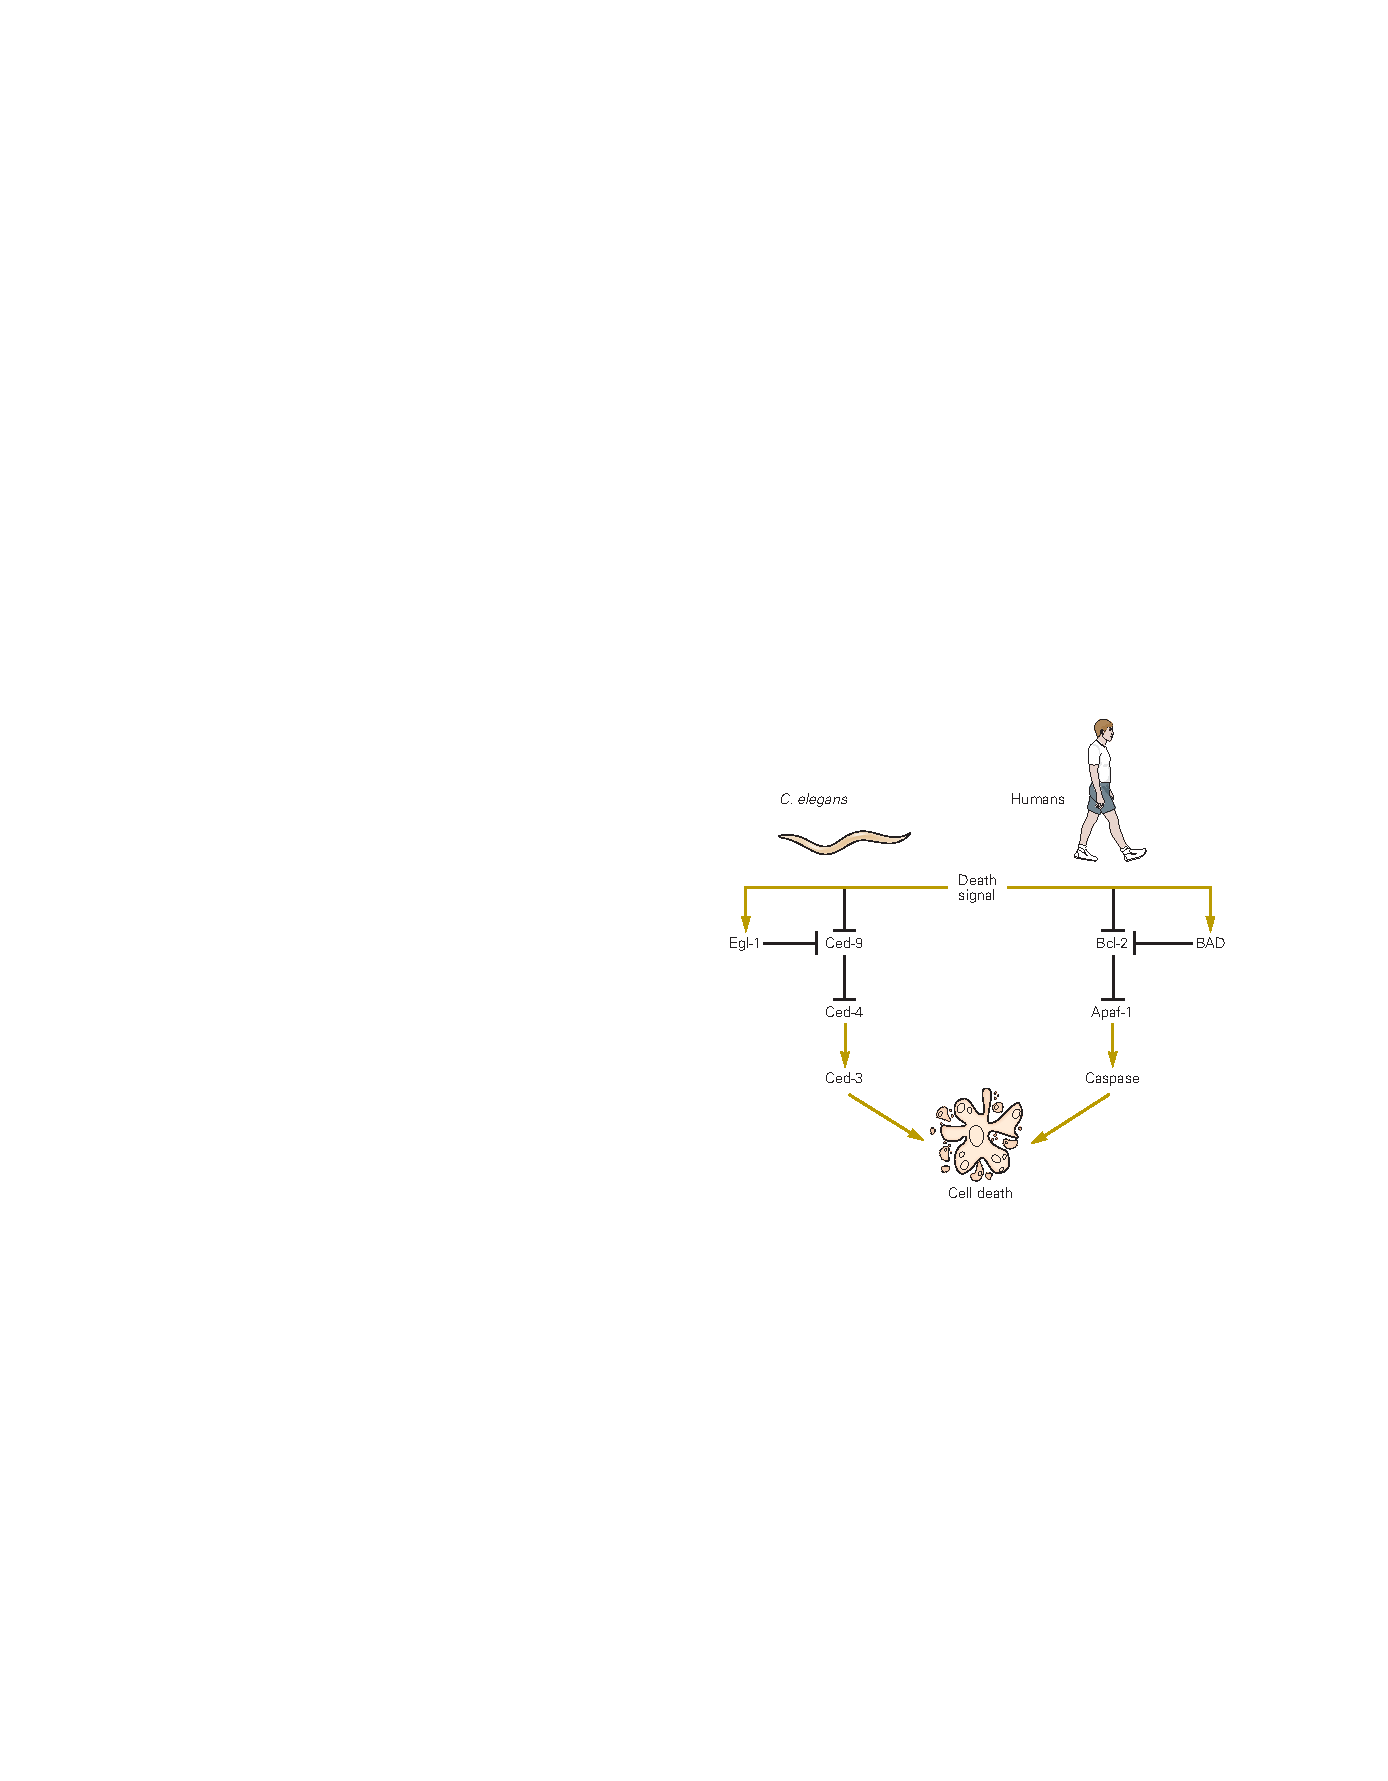
\includegraphics[width=0.89\linewidth]{chap46/fig_46_19}
	\caption{神经元和其他细胞表达一种保守的死亡程序。
	不同的细胞损伤会触发涉及一系列死亡效应基因的遗传级联反应。
	这些死亡基因和途径在从蠕虫到人类的物种进化过程中得到了保护。
	核心死亡途径激活一组蛋白水解酶,半胱天冬酶。
	\textit{半胱天冬酶}切割许多下游和必需的蛋白质底物(参见图~\ref{fig:46_20}),导致细胞通过称为细胞凋亡的过程死亡。
	对秀丽隐杆线虫的遗传分析表明,Ced-9 蛋白作用于上游并抑制 Ced-4 和 Ced-3 这两种促进细胞死亡的蛋白质的活性。
	Ced-9 的许多脊椎动物同源物,即 Bcl-2 蛋白家族,已被鉴定。
	其中一些蛋白质(例如 Bcl-2 本身)会抑制细胞死亡,但其他蛋白质会通过拮抗 Bcl-2 的作用来促进细胞死亡。
	Bcl-2 类蛋白作用于\textit{凋亡蛋白酶激活因子1}(Ced-4 的脊椎动物同系物)和半胱天冬酶(Ced-3 的脊椎动物同系物)的上游。}
	\label{fig:46_19}
\end{figure}


\begin{figure}[htbp]
	\centering
	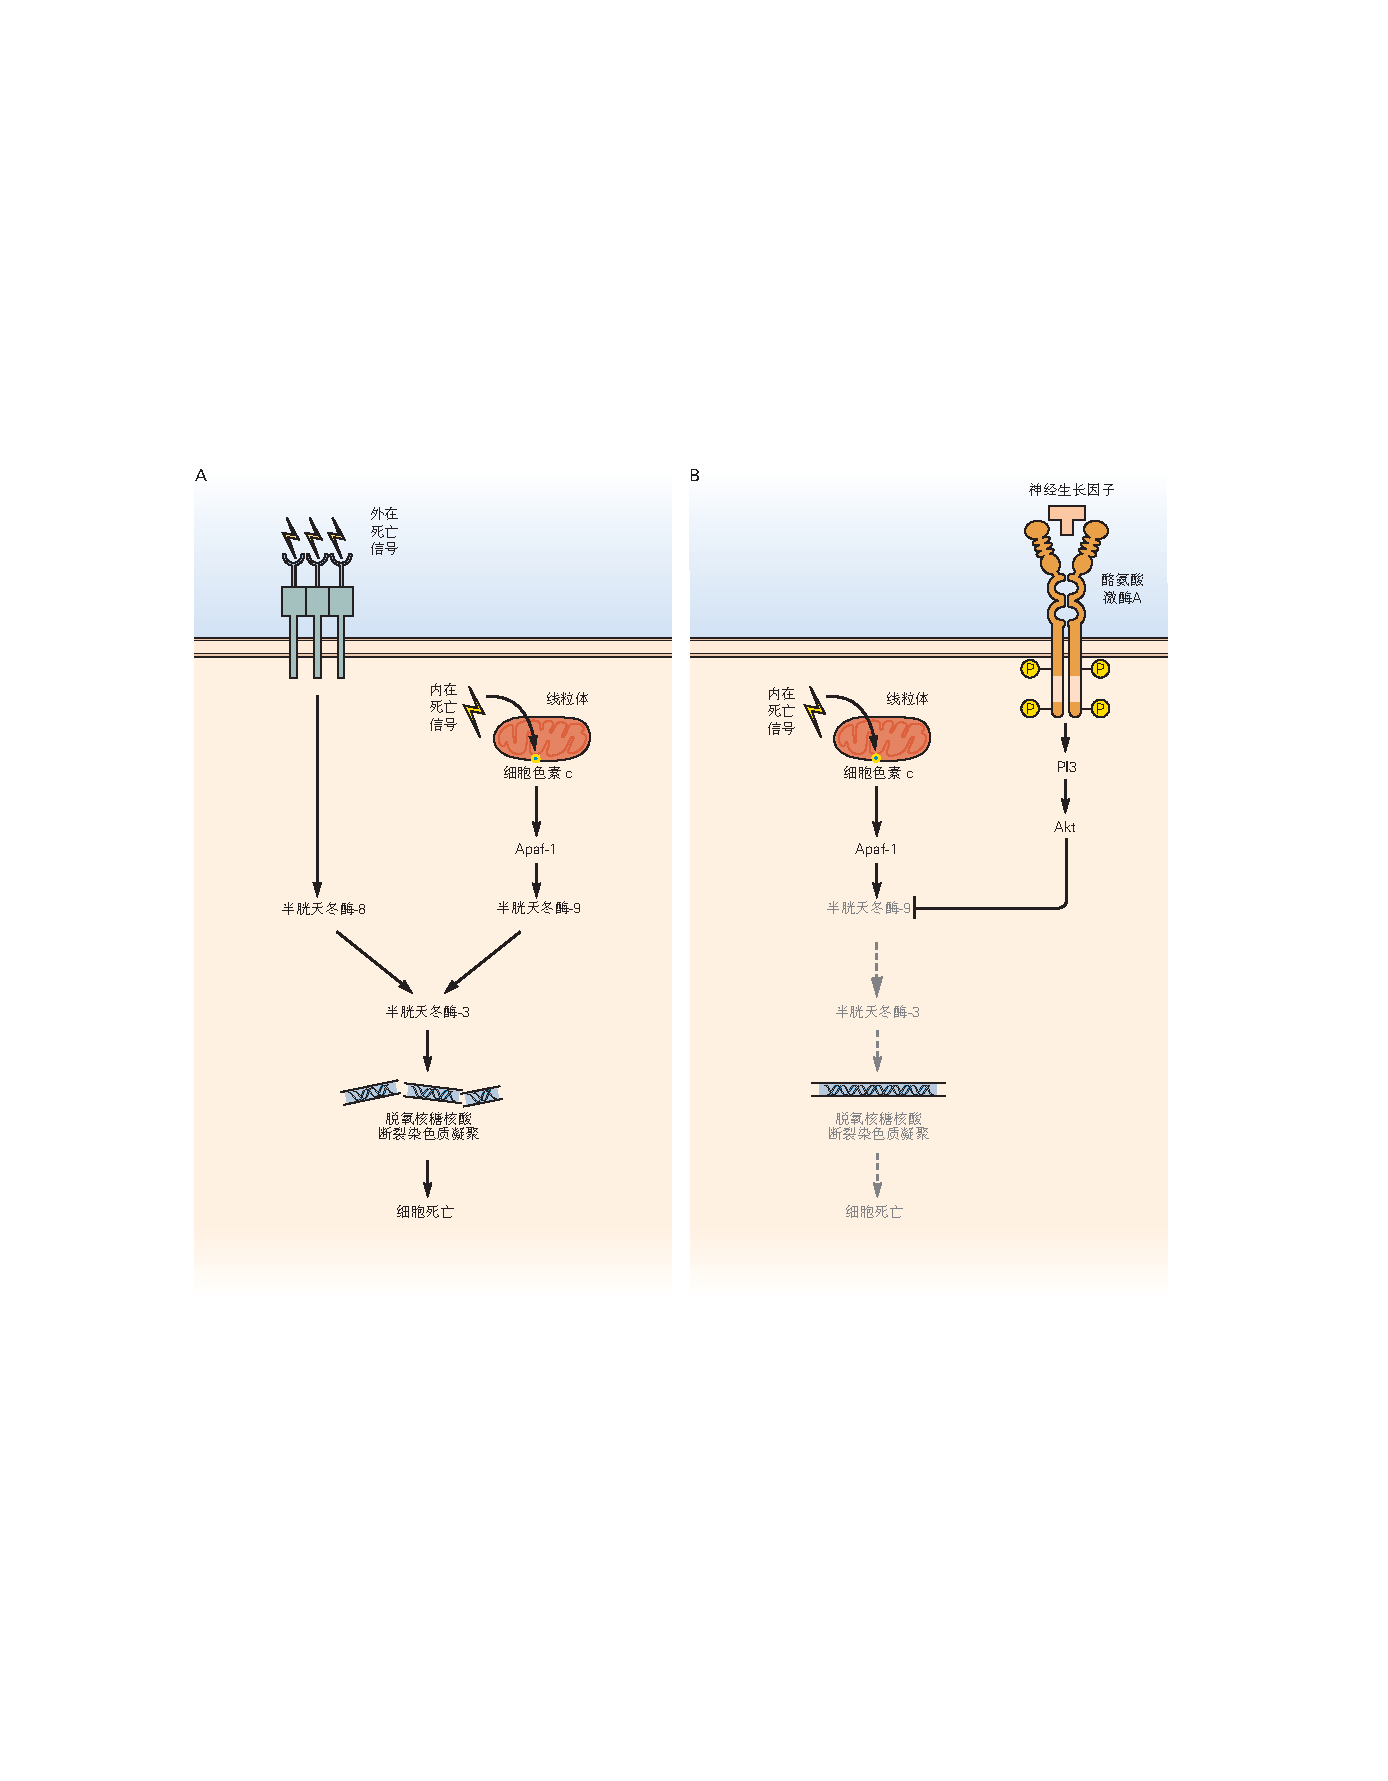
\includegraphics[width=1.0\linewidth]{chap46/fig_46_20}
	\caption{神经营养因子抑制半胱天冬酶活化和细胞死亡\cite{jesenberger2002deadly}。
		\textbf{A.} 两种类型的途径触发细胞死亡:表面膜死亡受体的外在激活和线粒体途径的内在激活。
		这两种途径都会导致 \textit{半胱天冬酶}-8 和 \textit{半胱天冬酶}-9 等 \textit{半胱天冬酶}的激活,从而启动蛋白水解切割级联反应,该级联反应会聚在 \textit{半胱天冬酶}-3 激活水平。
		半胱天冬酶前体的切割去除半胱天冬酶前结构域并产生蛋白水解活性酶构象。
		外在途径涉及配体激活死亡受体,例如肿瘤坏死因子受体 1 或 Fas/CD95。
		内在途径涉及应激诱导的信号,例如\textit{脱氧核糖核酸}损伤,这些信号启动线粒体膜间隙释放细胞色素 c。
		细胞色素 c 与\textit{凋亡蛋白酶激活因子1}结合并募集和激活 \textit{半胱天冬酶}-9。
		\textbf{B.} 神经营养蛋白与\textit{酪氨酸激酶}受体的结合会募集 PI3 激酶通路和 Akt,并通过抑制 \textit{半胱天冬酶}-9 来抑制细胞死亡通路。
		该通路在神经元发育过程中被神经营养因子抑制,这解释了为什么这些因子的撤除会导致细胞凋亡。}
	\label{fig:46_20}
\end{figure}


秀丽隐杆线虫中的细胞死亡途径在哺乳动物中是保守的。
类似的蛋白质和通路控制着中枢神经元和外周神经元的凋亡,实际上是所有发育中细胞的凋亡。
蠕虫 \textit{细胞死亡}-9 基因编码一种与哺乳动物 Bcl-2 家族成员相关的蛋白质,可保护淋巴细胞和其他细胞免于凋亡。
蠕虫 \textit{细胞死亡}-3 基因编码的蛋白质与一类称为半胱天冬酶的哺乳动物半胱氨酸蛋白酶密切相关。
蠕虫 \textit{细胞死亡}-4 基因编码一种蛋白质,该蛋白质在功能上与一种称为\textit{凋亡蛋白酶激活因子1}的哺乳动物蛋白质相关。


哺乳动物凋亡细胞死亡途径的工作方式类似于蠕虫途径(图~\ref{fig:46_20})。
伴随哺乳动物细胞凋亡的形态学和组织化学变化是由半胱天冬酶的激活引起的,半胱天冬酶切割细胞蛋白质中的特定天冬氨酸残基。
两类半胱天冬酶调节细胞凋亡:启动子半胱天冬酶和效应半胱天冬酶。 起始半胱天冬酶(\textit{半胱天冬酶}-8、-9 和 -10)切割并激活效应半胱天冬酶。
效应半胱天冬酶(\textit{半胱天冬酶}-3 和 -7)裂解其他蛋白质底物,从而触发细胞凋亡过程。
细胞中可能有 1\% 的蛋白质用作效应半胱天冬酶的底物。
它们的切割通过多种途径促进神经元凋亡:通过蛋白水解级联的激活、修复失活、\textit{脱氧核糖核酸}切割、线粒体透化和吞噬作用的启动。


哺乳动物神经元的存活取决于 Bcl-2 蛋白家族的抗凋亡和促凋亡成员之间的平衡。
一些 Bcl-2 蛋白如 BAX 和 BAK 增加线粒体外膜的通透性,导致细胞色素 c 等促凋亡蛋白释放到细胞质中。
细胞色素 c 的释放诱导\textit{凋亡蛋白酶激活因子1}结合并激活 \textit{半胱天冬酶}-9,导致效应 \textit{半胱天冬酶} 的切割和激活。
神经营养因子与其酪氨酸激酶受体的结合被认为会导致促进 Bcl-2 样活性的蛋白质底物磷酸化(图~\ref{fig:46_20}B)。
因此,从神经元中撤出神经营养因子会改变 Bcl-2 家族从抗凋亡到促凋亡成员的平衡,从而触发神经元的死亡。


\textit{半胱天冬酶}细胞死亡程序也可以被许多细胞损伤激活,包括\textit{脱氧核糖核酸}损伤和缺氧。
细胞外配体对细胞表面死亡受体(如 Fas)的激活导致 \textit{半胱天冬酶}-8 或 -10 的激活以及死亡效应蛋白(如 FADD)的募集。
将启动子半胱天冬酶募集到 Fas-FADD 复合物然后导致效应子半胱天冬酶的激活。
由于许多神经退行性疾病会导致细胞凋亡,因此正在研究抑制半胱天冬酶的药理学策略。



\section{要点}

1. 神经管心室表面附近的干细胞分裂扩张神经上皮。
然后进一步分裂产生中枢神经系统的神经元和神经胶质细胞以及放射状神经胶质细胞。


2. 放射状神经胶质突从脑室延伸至软脑膜表面。
放射状胶质细胞继续分裂形成神经元和星形胶质细胞。
在皮层中,它们还充当支架,新生兴奋性神经元在其上迁移到适当的层。


3. 神经元和胶质细胞命运之间的选择取决于从 Delta 家族配体到邻近细胞上 Notch 家族受体的信号。
最初,细胞同时表达 Notch 和 Delta。
Notch 的激活导致神经胶质命运,下调 Delta,这反过来又减弱了 Notch 对邻居的活动,促进它们分化为神经元。


4. 当皮层主要(兴奋性)神经元沿着放射状胶质细胞迁移时,它们以由内而外的顺序形成皮层层(第 6 层在第 5 层之前形成,依此类推)。
移民中断是导致智力障碍和癫痫的原因之一。


5. 与兴奋性神经元不同,前脑中间神经元出现在皮层下的神经节隆突中,然后切向迁移到皮层、基底神经节和其他前脑结构中。


6. 神经嵴细胞从神经管背侧尖端的源头通过体节和间充质迁移,形成感觉和自主神经元和神经胶质细胞,以及几种非神经细胞类型。


7. 对于主要神经元、中间神经元和外周神经元,沿迁移路径遇到的内在差异和线索相互作用以诱导不同转录因子组合的表达。
然后转录程序导致发育中的神经元多样化为多个类别和类型。


8. 与低等哺乳动物相比,灵长类动物,尤其是人类大脑的复杂性更高,部分原因是神经元祖细胞的数量更多,包括第二种类型的放射状神经胶质细胞。


9. 人类大脑研究能力的最新进展是发现可以从干细胞中产生称为大脑类器官的复杂神经元集合。
尽管它们无法获得成熟皮层的特征,但它们能够分析早期大脑发育及其障碍的某些方面,并可能有助于测试可能的治疗方法。


10. 神经元使用的神经递质被确定为转录程序的一部分,该程序赋予每种神经元类型以其定义特征。
然而,在某些情况下,包括电活动模式和荷尔蒙环境在内的外在因素会导致发射器切换。


11. 神经系统产生的神经元数量是成年期存活神经元的两倍。
多余的部分被从无脊椎动物到人类都保存下来的细胞死亡程序消除。


12. 营养因素在决定群体中哪些神经元存活或死亡方面起着至关重要的作用。
他们通过控制细胞死亡程序来控制生存。
在某些情况下,神经元似乎会竞争有限的神经营养因子供应;
细胞死亡程序在那些失去竞争的人中被激活。 


13. 体内产生多种营养因子,每一种只控制某些神经元类型的命运。
研究最透彻的称为神经营养因子(神经生长因子、脑源性神经营养因子、神经营养因子 3 和神经营养因子 4),结合并激活称为\textit{酪氨酸激酶}受体的激酶。


